\documentclass[preprint,11pt]{elsarticle}
\usepackage{epsfig,graphicx,amsmath,amssymb,verbatim,bm,amsfonts}
\usepackage{float}
\usepackage{tikz}
\usepackage{dcolumn}
\usepackage{xcolor}

%------------------------------------
% Just for adding readable todo notes
\usepackage[paperwidth=275.9mm, paperheight=279.4mm]{geometry} %regular letter size is 215.9 wide by 279.44 long
\setlength{\evensidemargin}{95mm}
\usepackage[colorinlistoftodos, textwidth=65mm, shadow]{todonotes}
%------------------------------------

\newcommand{\bq}{\begin{equation}}
\newcommand{\eq}{\end{equation}}
\newtheorem{lemma}{Lemma}[section]
\newtheorem{theorem}{Theorem}[section]
\newtheorem{remark}{Remark}[section]

% DLG comment inline command
\newcommand{\dlg}[1]{\todo[nolist,size=\small, color=green!40]{#1}}

\newcommand{\bU}{{\bf U}}
\newcommand{\bn}{{\bf n}}
\newcommand{\bx}{{\bf x}}
\newcommand{\bv}{{\bf v}}
\newcommand{\T}{{\mathcal T}}

\def\ljump{{[\![}}
\def\rjump{{]\!]}}

\def\lavg{{\{\!\{}}
\def\ravg{{\}\!\}}}

\def\3bar{{|\hspace{-.02in}|\hspace{-.02in}|}}
\setlength{\textwidth}{6truein} \setlength{\textheight}{8truein}
\voffset=-0.55truein
\hoffset=-0.65truein

\journal{Computer Physics Communications}
\begin{document}
\begin{frontmatter}
\title{A Sparse-Grid Discontinuous Galerkin Approach to Simulating Runaway Electron Dynamics}
%
\tnotetext[t1]{This manuscript has been authored in part by UT-Battelle, LLC, under contract DE-AC05-00OR22725 with the US Department of Energy (DOE). The US government retains and the publisher, by accepting the article for publication, acknowledges that the US government retains a nonexclusive, paid-up, irrevocable, worldwide license to publish or reproduce the published form of this manuscript, or allow others to do so, for US government purposes. DOE will provide public access to these results of federally sponsored research in accordance with the DOE Public Access Plan (http://energy.gov/downloads/doe-public-access-plan).} 
%
\author[1]{David L. Green}
\ead{greendl1@ornl.gov}
%
\author[1]{Diego B. Del-Castillo-Negrete}
\ead{delcastillod@ornl.gov}
%
\author[2]{Eduardo D'Azevedo}
%
\author[3]{Lin Mu\corref{cor1}}%\fnref{fn1}}
\ead{linmu@uga.edu}
%
\author[1]{Louis Wonnell}
\author[1]{Timothy Younkin}
\author[1]{B. Tyler McDaniel}
\author[1]{Harry Hughes}
%
\address[1]{Fusion Energy Division, Oak Ridge National Laboratory, Oak Ridge, TN 37831, USA}
\address[2]{Computer Science and Mathematics Division, Oak Ridge National Laboratory, Oak Ridge, TN 37831, USA}
\address[3]{Department of  Mathematics, University of Georgia, Athens,  GA 30602, USA}
%
\cortext[cor1]{Corresponding author}
%
\begin{abstract}
Text goes here.
\end{abstract}
%
\begin{keyword}
Fokker-Planck collision model, runaway electrons, discontinuous Galerkin method, sparse grids finite element methods.
\end{keyword}
%
\end{frontmatter}


\section{Introduction}
\label{sec:intro}
{\tiny\color{red} Motivation\\}
The simulation of collisional transport is ubiquitous to many fields of science. Here, our focus is the velocity-space transport of electrons in a magnetized plasma subject to an accelerating electric field. Such Fokker-Planck type models are routinely employed in plasma physics to describe the dynamics of velocity-space diffusion due to collisions of the species of interest with either itself or the other charged particle species present. While several codes exist to simulate such phenomena (e.g., CQL3D, LUKE, SCEAM code, TDS codes, CODE code), these are typically limited to 2D (0x-2v) or 3D (1x-2v). Since there is reason to simulate the dynamics in 4D (2x-2v) or even 5D (3x-2v), for example the non-bounce averaged dynamics of the runaway electron population in Tokamak devices due to ... \todo{diego} or finite ion orbit effects in the dynamics of radio frequency heating, we have begun exploring the application of sparse-grids \cite{} to enable the solution of such high dimensional PDEs within the bounds of routinely available computational resources. In this paper we test this sparse-grid approach within the framework of the Discontinuous-Galerkin (DG) finite-element method for a 2D (0x-2v) model with a linear collision operator for a single species colliding with a Maxwellian background.  
      
{\tiny\color{red} Review of DG and its advantages for plasma physics\\}
Discontinuous Galerkin methods were first introduced by Reed and Hill \cite{ReedHill1973} for linear neutron transport equations in 1973. As a class of finite-element (FE) methods, DG methods \cite{HesthavenWarburton2008} adopt finite-element type meshes for spatial discretization and inherit their geometrical adaptability. However, in contrast to continuous nodal FE methods, they allow the solutions to be discontinuous across the element interfaces by using discontinuous basis functions over the elements and defining numerical fluxes at the element interfaces. The DG basis functions are local to each element and therefore independent of those in neighboring elements, which offers inherent parallelism and allows the use of general meshes, including those with hanging nodes. These advantages of DG methods, combined with a capability for higher-order approximations, have resulted in significant interest in their application in various physical sciences. In plasma physics specifically, several recent efforts to apply DG include the Gykell framework \cite{}, \todo{david} . Due to the embedded flexibility in designing specific numerical fluxes for achieving different features, DG methods can also produce numerical solutions with desired physical properties preserving features such as mass conservation. These conservation, parallelism, and ... \todo{david} properties are of particular interest to plasma physics applications and motivate our choice of DG as the framework within which to test our sparse-grid approach.  

{\tiny\color{red} Review of sparse-grids and sparse-grid DG\\}
While DG exhibits many advantages, it still suffers from the ``curse of dimensionality'' where the number of Degrees of Freedom (DoF) scales as $\mathcal{O}(h^{-d})$ where $d$ and $h$ denote dimensionality of the problem and the finest mesh size respectively. Sparse-grids \cite{Bungartz2004} offer the potential to improve this scaling in DoF to $\mathcal{O}(h^{-1}|\log_2 h|^{d-1})$ by utilizing a finite-element space which is based on a truncated tensor product. For standard sparse-grids (i.e., non-adaptive) there are several choices as to how to truncate, but all result in removing some part of the untruncated or ``full-grid'' finite-element space responsible for representing the higher order mixed derivatives which ideally are not required by the solution. Previous efforts towards DG methods atop sparse-grids include application to elliptic equations \cite{wang2016sparse}, transport \cite{GuoCheng2017}, Vlasov-Poisson \cite{guo2016sparse,guo2017adaptive}, and Vlasov-Maxwell equations \cite{tao2019sparse} ... \todo{add EU refs / david}. These sparse-grid finite-element approaches have demonstrated significant computational cost savings in both storage and compute time while preserving similar accuracy as that for full-grid simulations. In this paper, we explore the implementation of sparse-grid DG methods for the Fokker-Planck model for collisional plasma transport in 2D.

{\tiny\color{red} Summary of rest of manuscript\\}
In section~\ref{sec:Mod} we desribe the physics model for simplified runaway electron dynamics, followed  by a description and testing of the full-grid DG discretization in 1D and 2D in section~\ref{sec:full-grid-scheme}. The sparse-grid implementation is described and tested in section~\ref{sec:sparse-grid-scheme} with future work and conclusions discussed in section~\ref{sec:future-work}.

\section{Physics Model}
\label{sec:Mod}
%
For the purposes of this paper we assume that the dynamics of the distribution function of the runaway electrons, $f$, is described by the following relativistic Fokker-Planck model
%
\bq
\label{fokkerplanckmodel}
\frac{\partial f}{\partial t}=  {\cal C} \{ f \} +E\{f\} + {\cal R}\{f\}
\eq
%
where ${\cal C} \{ f \}$ is the collision operator, $E\{f\}$ is the electric field acceleration operator, and ${\cal R}\{f\}$ is the radiation damping operator. In flux conserving form, 
%
\bq
\label{eq:fluxconservform}
\frac{\partial f}{\partial t}= - \nabla \cdot \left [ {\bf \Gamma}^{\cal C}+ {\bf \Gamma}^E+ {\bf \Gamma}^{\cal R}\right] 
\eq
%
where ${\bf \Gamma}^{\cal C}$ is the collisional flux, ${\bf \Gamma}^E$ is the electric field acceleration flux, and ${\bf \Gamma}^{\cal R}$ is radiation damping flux. The distribution function $f$ depends on time, $t$, and the phase-space variables $\xi=\cos \theta \in [-1,1]$ \todo{diego - why choose $\xi$ and not $\theta?$} and $p\in [0, \infty)$ but is independent of any spatial coordinate. The phase-space variables are based on a spherical velocity-space coordinate system  $(p,\theta,\phi)$ where $p$ is relativistic momentum, $\theta$ is the angle between a background confining magnetic field, and $\phi$ is the angular position around that field. Transforming these coordinates back to Cartesian is via the standard expressions $p_x= p \sin \theta \cos \phi$, $p_y= p \sin \theta \sin \phi$, $p_z= p \cos \theta$. From now on it will be assumed that the dynamics are also independent of $\phi$. In these $(p,\xi)$ coordinates, the divergence of a vector ${\bf V}=V_p \hat {\bf e}_p+V_\xi \hat {\bf e}_\xi$ is given by
%
\bq
\nabla \cdot {\bf V}=\frac{1}{p^2}\left[ \frac{\partial }{\partial p} \left( p^2 V_p\right) 
+ p  \frac{\partial }{\partial \xi} \left( \sqrt{1-\xi^2}  V_\xi \right) 
\right ] \, .
\eq
%
We are using non-dimensional variables according to which the relativistic momentum has been normalized by $m \tilde{v}_T$, where $\tilde{v}_T=\sqrt{2 \tilde{T}/m}$ is the thermal speed, with $\tilde{T}$ a plasma reference temperature and $m$ the electron mass. The time has been normalized using the thermal collision frequency 
$\tilde{\nu}_{ee}=e^4 \tilde{n}\ln \tilde{\Lambda}/(4 \pi \epsilon_0^2 m^2 \tilde{v}_T^3)$, where $e$ is the absolute value of the electron charge, $\epsilon_0$ is the vacuum permitivity, and $\tilde{\Lambda}$ is the Coulomb logarithm for a plasmas with reference temperature $\tilde{T}$ and reference density $\tilde{n}$. The electric field has been normalized using $\tilde{E}_D/2$ where $\tilde{E}_D= e^3 \tilde{n}\ln \tilde{\Lambda}/(4 \pi \epsilon_0^2 \tilde{T})$ is the Drecier field. This non-dimensionaliztion leads to the following model for the Fokker-Planck fluxes
%
\begin{eqnarray}
\label{eq:collisionflux}
{\bf \Gamma}^{\cal C}&=& -\left ( C_A \frac{\partial f}{\partial p} + C_F f \right) \hat {\bf e}_p-
\frac{C_B}{p^3} \sqrt{1-\xi^2} \, \frac{\partial f}{\partial \xi}\, \hat {\bf e}_\xi \\
\label{eq:electricfieldflux}
{\bf \Gamma}^{E}&=& E \left(\xi f  \hat {\bf e}_p + \sqrt{1-\xi^2}  \, f\, \hat {\bf e}_\xi \right) \\
\label{eq:radiationflux}
{\bf \Gamma}^{\cal R}&=& -\frac{\gamma p \left(1-\xi^2\right)}{\tau} f \, \hat {\bf e}_p +
\frac{p \xi}{\tau \gamma} \sqrt{1-\xi^2}\, f\, \hat {\bf e}_\xi \, ,
\end{eqnarray}
%
with the collisional term coefficients being 
%
\begin{eqnarray}
C_A (p) &=& \bar{\nu}_{ee} \, \bar{v}_T^2 \,\,\frac{\psi(x)}{x}
 \\
C_B (p)&=& \frac{1}{2} \,\bar{\nu}_{ee} 
\, \bar{v}_T^2 \, \, \frac{1}{x}  \left[ Z + \phi(x)- \psi(x) + \delta^4  \frac{x^2}{2} \right]\\
C_F (p)&=&2\,\bar{\nu}_{ee}  \, \bar{v}_T \, \psi(x) \, .
\end{eqnarray}
%
where
%
\bq
\phi(x)=\frac{2}{\sqrt{\pi}} \int_0^x e^{-s^2} ds \, ,\qquad
\psi(x)=\frac{1}{2 x^2} \left[ \phi(x)-x \frac{d \phi}{dx} \right] 
\eq
%
\bq
x=\frac{1}{\bar{v_T}} \frac{p}{\gamma}\, , \qquad
\gamma=\sqrt{1+\left(\delta p\right)^2} \, ,
\eq
and
\bq
\bar{v_T}=\sqrt{\frac{T}{\tilde{T}}}\, , \qquad \bar{\nu}_{ee}=\left(\frac{\tilde{T}}{T}\right)^{3/2}\, \frac{\ln \Lambda}{\ln \tilde{\Lambda}} \, , \qquad  \delta=\frac{v_T}{c}=\sqrt{\frac{2 T}{m c^2}} \, .
\eq
%
Note that for the normalization we are using the reference plasma parameters $\tilde{n}$, $\tilde{T}$ and 
$\tilde{\Lambda}$. In addition, we have $n$, $T$ and $\Lambda$ that denote the actual plasma density, temperature,  and Coulomb logarithm, which might depended explicitly on time. When considering time-independent plasma states we can take $\tilde{n}=n$, $\tilde{T}=T$ and 
$\tilde{\Lambda}=\Lambda$. 


\subsection{Boundary Conditions}
\label{sec:BCs}
In the numerical implementation, the semi-infinite domain is truncated to the rectangle $[-1,1] \times [0, p_{max}]$. The regularity condition at $p=0$ requires
%
\bq
\label{momentumregularity}
f(p\rightarrow 0,\xi,t) \sim A p^m \, ,
\eq 
%
\todo{should there be a + on the 0 above?} where $A$ is a constant and  $m \geq 2$. The regularity condition in the $\theta \in (0, \pi)$ variable requires
%
\bq
\label{angregularity}
f (p, \theta \rightarrow  0^+,t) \sim A + B\, \theta^m \, , \qquad
f (p, \theta \rightarrow  \pi^-,t) \sim C + D (\pi-\theta)^m\, ,
\eq
where $A$, $B$, $C$ and $D$ are constants and $m \geq 2$. These regularity conditions imply that at the boundaries
%
\bq
\label{boundaryconditions}
\left. \partial_p f \right|_{p=0}=0 \, , \qquad \partial_\theta f \left. \right |_{\theta=0, \pi}=0 \, .
\eq
%
Note that {\em{any}} function of $\xi = \cos \theta$ satisfies the regularity conditions in $\theta$ because near $\theta=0$, $\xi \sim 1 -\theta^2/2$ and 
near $\theta=\pi$, $\xi \sim -1 +(\pi-\theta)^2/2$. \todo{so what is the BC on xi? there really isn't one? we certainly implement one?} These conditions imply that
%
\bq
\label{fluxboundaries}
\left. {\bf \Gamma} \cdot \hat {\bf e}_p \right|_{p=0}=0 \, , \qquad 
\left. {\bf \Gamma} \cdot \hat {\bf e}_\xi \right|_{\xi=-1}=0 \, , \qquad 
\left. {\bf \Gamma} \cdot \hat {\bf e}_\xi \right|_{\xi=1}=0 \, .
\eq
%
The boundary condition at $p=p_{max}$ can no be inferred from the coordinate system, but can reasonably be set in several ways. Here, and unless otherwise specified we choose 
%
\bq
\label{pmaxboundary}
f(p=p_{max}, \xi, t)=0 \, ,
\eq
%
which is  a good approximation to the physical boundary condition $f(p\rightarrow \infty , \xi, t) \rightarrow 0$, provided that $p_{max}\gg 1$. 
%
% DLG - Since we do not use this mixed BC in the presented work i am commenting this out. 
%Note that in this case we cannot guarantee that $\left. {\bf \Gamma} \cdot \hat {\bf e}_p \right|_{p=p_{max}}=0$, because the boundary condition defined in equation \ref{pmaxboundary}. But, if  a vanishing flux is needed for the DG algorithm, we can then use the mixed boundary condition
%\bq
%\label{mixedboundary}
%\left. -C_A \frac{\partial f}{\partial p} + \left[ E \xi - C_F  -\frac{\gamma p \left(1-\xi^2\right)}{\tau_R}  \right] f \right|_{p=p_{max}} =0 \, ,
%\eq
%that will imply
%\bq
%\label{fluxpmaxboundary}
%\left. {\bf \Gamma} \cdot \hat {\bf e}_p \right|_{p=p_{max}}=0 \, .
%\eq


\section{Full-grid (1D and 2D) Discretization and Testing}
\label{sec:full-grid-scheme}
%
In this section we describe the spatial and temporal discretization for our DG scheme on the {\em{full-grid}} finite-element space. The {\em{sparse-grid}} discretization is described later in Section~\ref{sec:sparse-grid-scheme}.


\subsection{1D Finite Element Space}
\label{sec:1D-FE-space}
%
We first review the hierarchical decomposition of a piece-wise polynomial space in one dimension on the interval $I=[0,1]$. Our notation follows the original DG sparse-grid paper \cite{WangTangGuoCheng}. A set of nested grids are defined on this interval by $2^n$ uniform cells with grid size $h = 2^{-n}$ as $I_j^n = (h_nj,h_n(j+1))$ where $j=0,\dots,2^n-1$ for any integer $0\le n\le N$. The level within the hierarchy is denoted $n$, to maximum depth of $N$. The nested piece-wise polynomial spaces are denoted as:
%
\begin{eqnarray}
V_k^n:=\{v:v\in P_k(I_j^n),\forall j=0,\dots,2^n-1\},\label{polynomialspace}
\end{eqnarray}
where $P_k(I_j^n)$ denotes the piece-wise polynomials of degree at most $k$ on the line segment $I_j^n$.  
%
\begin{figure}[H]
\centering
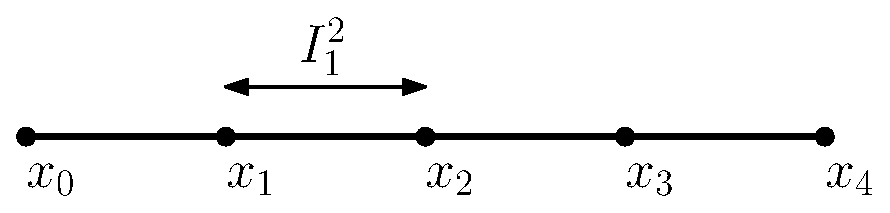
\includegraphics[width=.4\textwidth]{FIGURES/Interval_1D}
\caption{Illustration of one dimensional grid for $I_j^2$ ($0\le j\le 3$) with grid level $n = 2$.}
\end{figure}
%
{\tiny\color{red} Recursive generation of the heirarchical basis?\\}
The subspace $W_k^n$, can be defined as the orthogonal complement of $V_k^{n-1}$ in $V_k^n$ with respect to the $L^2$ inner product, such that $V_k^{n-1}\bigoplus W_k^n = V_k^n$ and $W_k^n\perp V_k^{n-1}$. By denoting $W_k^0:=V_k^0$, the standard piecewise polynomial space $V_k^N$ on $\Omega$ can be represented by a hierarchical form \todo{For LIN - It's not clear to me what the hierarchical form means. What is the kronecker product with on the RHS? {\color{blue}Lin: This is not Kronecker product. It is complement plus, meaning we adding up all the subspaces}} 
%
\begin{equation}
\label{hierarhicalform}
V_k^N = \bigoplus_{0\le n\le N}W_k^n. 
\end{equation}
%
We denote the hierarchical nested finite element basis funcions as $\phi_{\kappa,j}^n(x)$, with $0\le\kappa\le k,0\le n\le N, 0\le j\le 2^n-1.$ Figure~\ref{Fig:HarBasis} plots the piece-wise constant finite element basis $\phi_{\kappa,j}^n(x)$ for the finite element space $V_0^3.$\todo{I don't understand how someone would generate the figure below from this info - where does the discontinuity come from?} We choose to employ a high order polynomial basis in the form of the multiwavelets introduced in \cite{}. An example of the our multiwavelet basis is illustrated in Fig.~\ref{} for various polynomial orders \todo{Lin or David - insert figure showing the actual basis we use for various orders}. 
%
\begin{figure}[H]
\centering
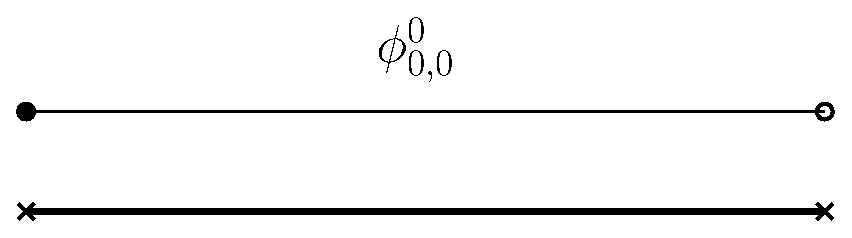
\includegraphics[width=.35\textwidth]{FIGURES/V00-basis}\\
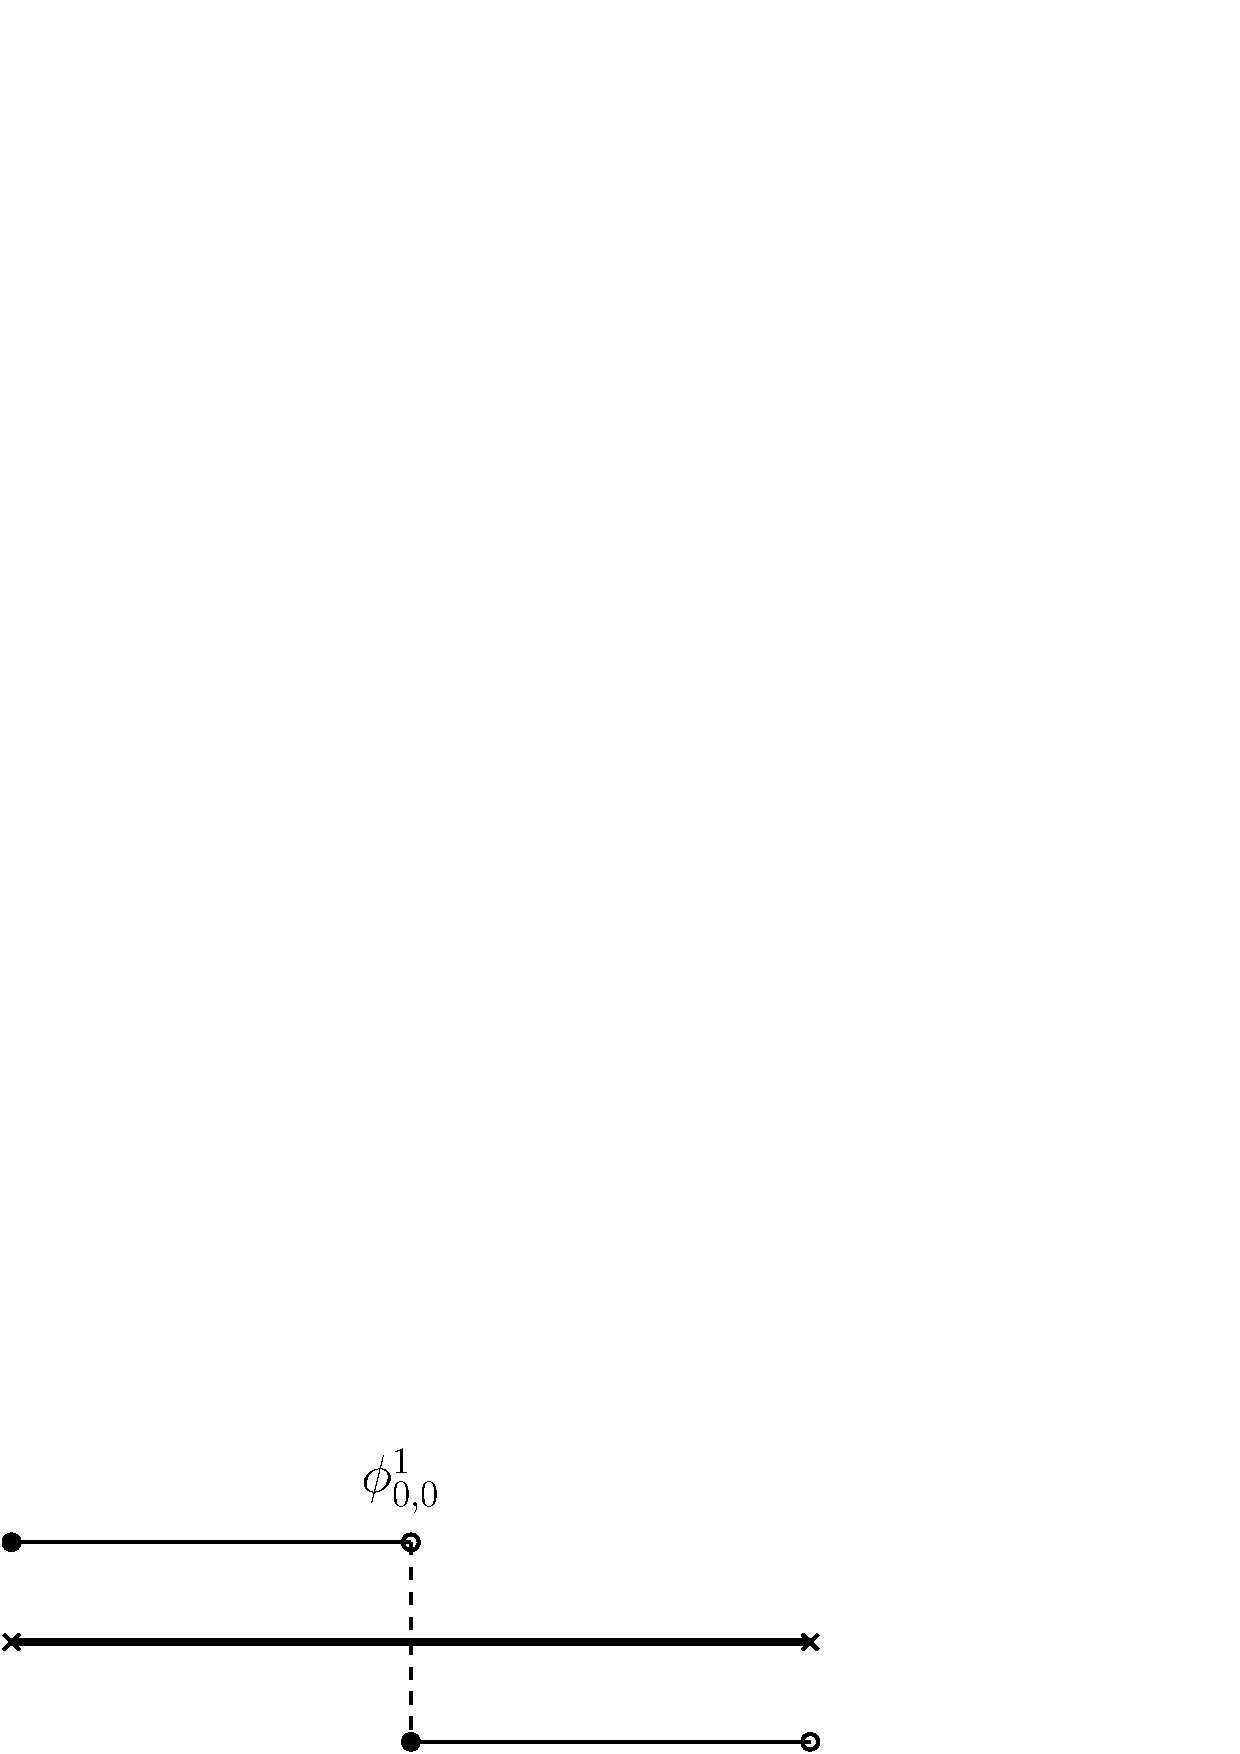
\includegraphics[width=.35\textwidth]{FIGURES/V01-basis}\\
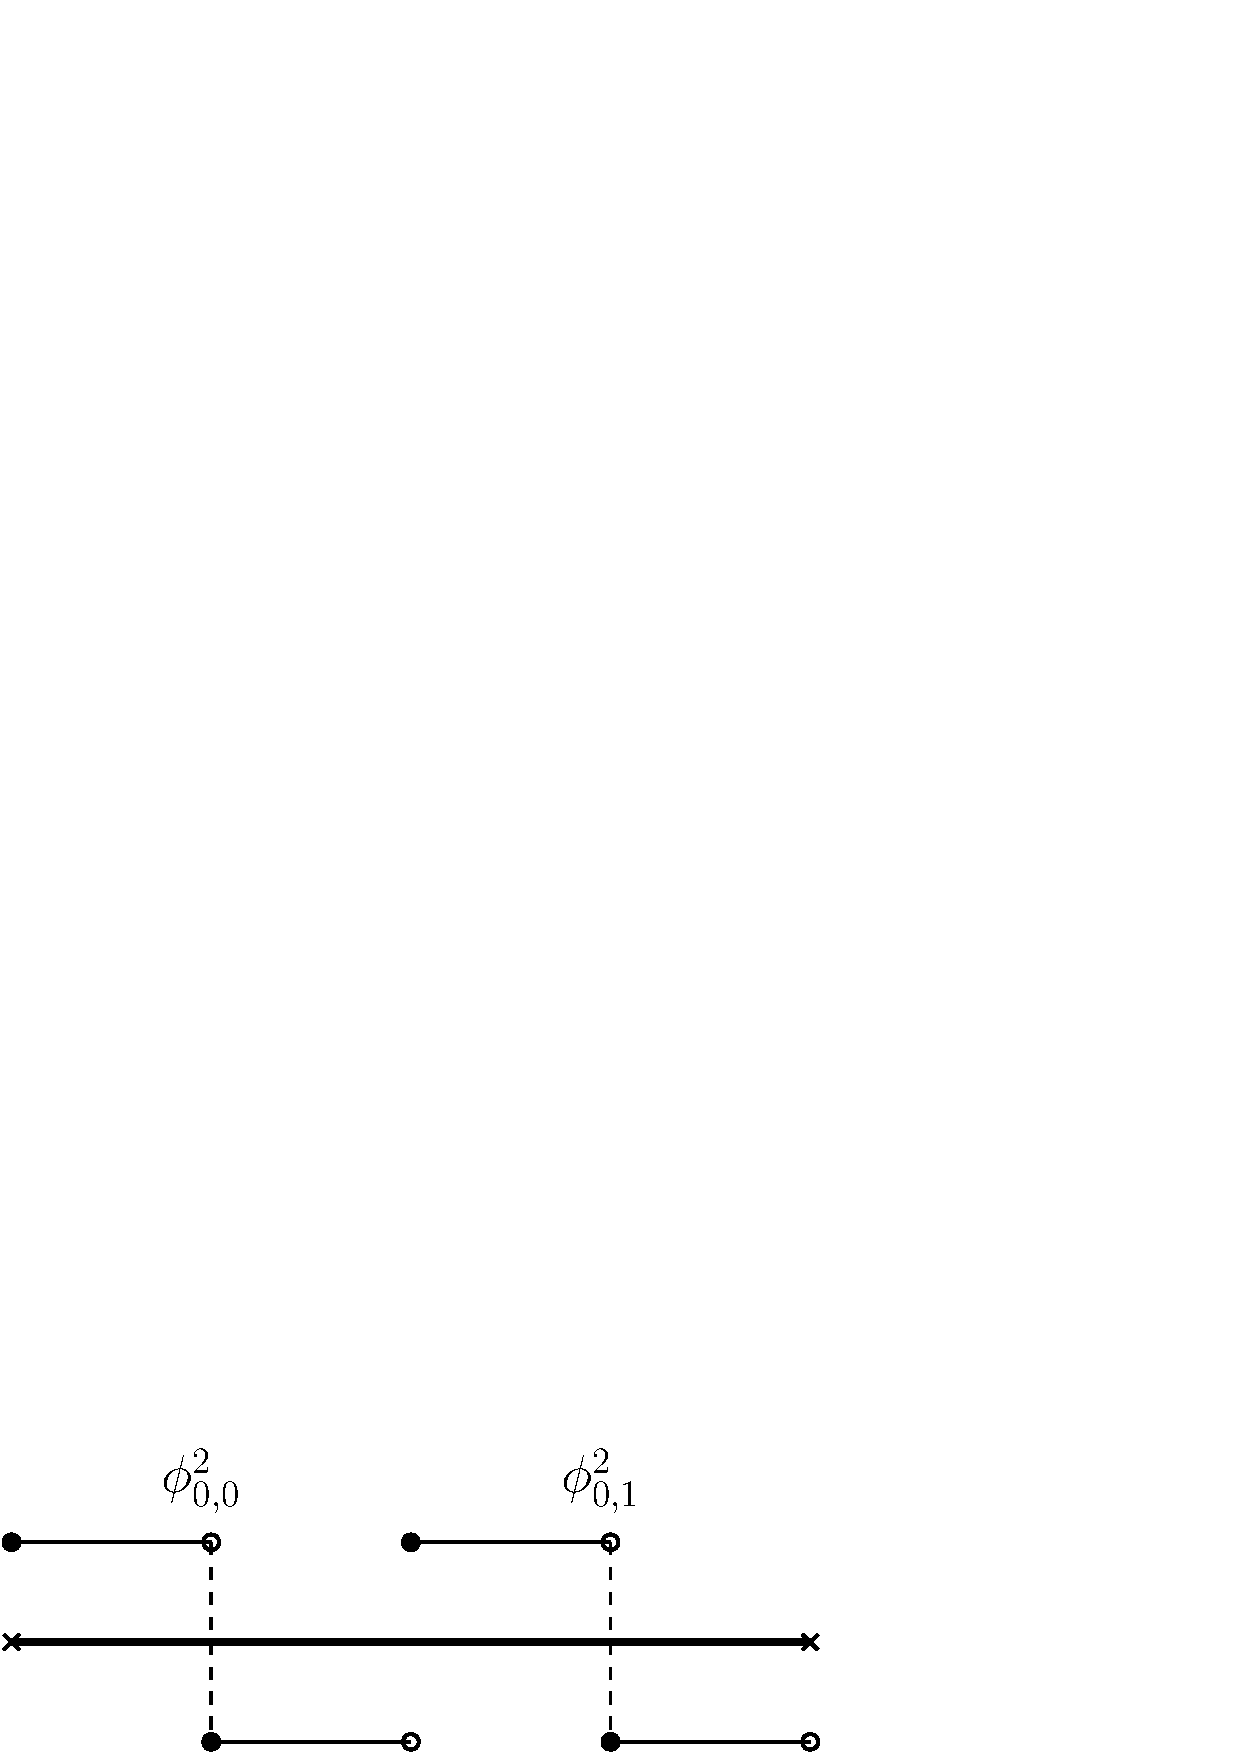
\includegraphics[width=.35\textwidth]{FIGURES/V02-basis}\\
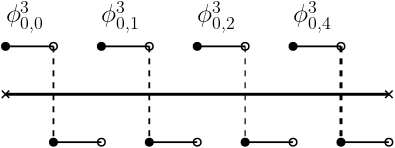
\includegraphics[width=.35\textwidth]{FIGURES/V03-basis}
\caption{Illustration of one dimensional hierarchical basis $\phi_{\kappa,j}^n(x)$ belongs to finite element space $V_{0}^3$ for degree $k = 0.$.}\label{Fig:HarBasis}
\end{figure}
%
\vskip.1in
- Notes on how the basis functions are created. Still need more on this.  \todo{**LIN**}


\subsubsection{Notations for discontinuous functions}
In this sub-section, we will review the notations in the DG finite element space. Without loss of generality, we assume a partition of domain $\Omega$ as $\mathcal{T}_h$ into a finite number of cells. Here, we will restrict the cells as line segments in a one-dimensional domain or Cartesian meshes with tensor-structure in a two-dimensional domain. Assume each element can be denoted as $K = K_{x_1}\times K_{x_2}$.
Let $\mathcal{T}_h:=\cup K$, $\mathcal{E}_h=\cup_{K\in\mathcal{T}_h} \partial K$ as the interfaces for all the elements $K$, and $\mathcal{E}_h^0$ as the interior edges. Also, we shall denote $\mathcal{T}_h = \mathcal{T}_{h,x_1}\times\mathcal{T}_{h,x_2}$\todo{DLG : I have no idea what this is trying to tell me. Will need to ask Lin. Also, it appears to have some 2D info, so likely needs to be moved outside this 1D section.}. 

For any edge $e=K^+\cap K^-\in\mathcal{E}_h^0$, %with $\bn^\pm$ as the outward unit normal to $\partial K^\pm$,
we define the jump $\ljump . \rjump$ and average $\lavg . \ravg$ operators for both vector valued functions $\bU$ and scalar valued functions $u$ across the edge $e$ as
%
\begin{eqnarray}
\ljump\bU\rjump = \bU^- - \bU^+,\
\ljump u \rjump=u^- - u^+,
\end{eqnarray}
%
and 
%
\begin{eqnarray}
\lavg\bU\ravg=\frac{1}{2}\left(\bU^++\bU^-\right),\text{ and }\lavg u\ravg=\frac{1}{2}\left(u^++u^-\right).
\end{eqnarray}
%
For cases where the element edges are on the domain boundary $\partial\Omega$ (i.e., $e\in\partial\Omega$), the jump and average operators are defined as $\lavg\bU\ravg = \bU|_e$, $\ljump\bU\rjump = \bU|_e$, $\lavg u \ravg = u|_e$, and $\ljump u\rjump = u|_e$. 


\subsection{Numerical Scheme for 1D Pitch Angle Dynamics}
\label{sec:1D-tests}
In this section we shall first present some special cases of the Fokker-Planck equation with analytical solutions.  These solutions will be used in the numerical test to verify the code and study the stability and convergence properties of the proposed algorithm.
\label{sec:1D-pitch}
%
In this section we implement and test the operators which describe the pitch angle  dynamics. For this purpose we retain only the differential operators and those parts of their coefficients which are independent variables (i.e., reduce the complicated physical coefficients of Eq.~\ref{eq:collisionflux} through \ref{eq:radiationflux} by setting $C_A=C_F=C_B=\gamma=\frac{p}{\tau}=1$). The resulting expression is 
%
\begin{eqnarray}
\label{fullpitchangleeq}
\frac{\partial f}{\partial t}=-E\frac{\partial}{\partial\xi}[(1-\xi^2)f]+C\frac{\partial}{\partial\xi}[(1-\xi^2)\frac{\partial f}{\partial\xi}]-R\frac{\partial}{\partial\xi}[\xi(1-\xi^2)f],
\end{eqnarray}
%
where $E,C,$ and $R$ are piece-wise constants.  
%
{\tiny\color{red} LDG vs Recovery method for diffusion terms\\}
For such a convection-diffusion system we utilize on a generalization of the original DG framework, introduced by  Cockburn and Shu in \cite{CockburnShu1998}, named the local discontinuous Galerkin (LDG) finite element method which allows for diffusion operators. The numerical performance of LDG and a comparison with DG is given in \cite{Castillo2002,Castillo2006}. Reviews of several other approaches to diffusion operators within the framework of DG are given in  \cite{cockburn2001runge,zhang2003analysis}. Similar to DG method, the LDG method is locally conservative, and thus is very attractive for practical transport computations. We note that there are also the more recent recovery discontinuous Galerkin (RDG) approaches to diffusion problems as introduced by Van Leer in \cite{VanLeerNomura2005} and extended to the compressible Navier-Stokes equations by Lo in \cite{LoVanLeer2011}. In the RDG method, an auxiliary variable is used to recover the value of the unknown and its derivative at cell interfaces via a fitting in the L2 sense of a continuous function. RDG has the advantage of achieving exceedingly high convergence rates (up to $3k+2$ in the cell-average error, where $k$ is the degree of the polynomial basis). However, in this paper, we shall employ the LDG scheme for the associated diffusion operators and leave an RDG implementation for future versions of our code.

Following the LDG approach, we rewrite equation \ref{fullpitchangleeq} as the following system of two first order equations
%
\begin{align}
	\dfrac{\partial f}{\partial t} &= -E\dfrac{\partial}{\partial\xi}[(1-\xi^2)f]+C\dfrac{\partial}{\partial\xi}q-R\dfrac{\partial}{\partial\xi}[\xi(1-\xi^2)f],\label{eq:pitch-pde1}\\
	q &= (1-\xi^2)\dfrac{\partial f}{\partial\xi}. \label{eq:pitch-pde2}
\end{align}
%
Denoting the finite element space by $V_h = V_k^N$ for the $\xi$ variable, multiplying both sides of equations \ref{eq:pitch-pde1} by a test function $v$ and both sides of equation \ref{eq:pitch-pde2} by a test function $w$, and integrating (denoted by the inner product operator $\left(.,.\right)$ below) over the cell $I_j^N$ ($j = 0,\cdots,2^N-1$) using integration by parts, implies the following numerical scheme for $f_h\in V_h$ and $q_h\in V_h$:
%
\begin{eqnarray}
\label{numericalschemepitchangle1}
(\dfrac{\partial f_h}{\partial t},v) &=& \mathcal{E}_{\xi}(f_h,v)+\mathcal{C}_{\xi}(q_h,v)+\mathcal{R}_{\xi}(f_h,v),\ \forall v\in V_h\\
\label{numericalschemepitchangle2}
(q_h,w)&=& \mathcal{D}_{\xi}(f_h,w),\ \forall w\in V_h,
\end{eqnarray}
%
where the bi-linear forms are defined as \todo{why are all the bi-linear forms below (w,v)? I would have expected then to be (u,v) and (u,w) or some other symbol for the basis expansion of f and q?{\color{blue}By Lin: I am using the variables w and v to define the more general formulation of the following terms.}}:
%
\begin{eqnarray}
\mathcal{E}_{\xi}(w,v) &=& \sum_{K_{\xi}\in \mathcal{T}_{h,\xi}}\int_{K_\xi}(E(1-\xi^2)w)\frac{\partial v}{\partial\xi} d\xi+\sum_{j=0}^{2^N} \left[\left\{\widehat{ E(1-\xi^2){w}}\right\}\ljump v\rjump\right]_{\xi_j}, 
\\
\mathcal{C}_{\xi}(w,v) &=& -\sum_{K_{\xi}\in \mathcal{T}_{h,\xi}}\int_{K_{\xi}}Cw\frac{\partial v}{\partial\xi}d\xi+
\sum_{j=0}^{2^N} \left[\left\{ \widehat{Cw}\right\}\ljump v\rjump\right]_{\xi_j},
\\
\mathcal{R}_{\xi}(w,v) &=&
\sum_{K_{\xi}\in \mathcal{T}_{h,\xi}}\int_{K_{\xi}}(\xi(1-\xi^2)w)\frac{\partial v}{\partial\xi}d\xi+
\sum_{j=0}^{2^N} \left[\left\{ \widehat{R\xi(1-\xi^2){f}}\right\}\ljump v\rjump\right]_{\xi_j},
\\
\mathcal{D}_{\xi}(w,v)&=&
-\sum_{K_{\xi}\in \mathcal{T}_{h,\xi}}\int_{K_{\xi}}w\frac{\partial}{\partial\xi}\left[(1-\xi^2)v\right]d\xi+
\sum_{j=0}^{2^N} \left[\{ \widehat{w}\}\ljump(1-\xi^2)v\rjump
\right]_{\xi_j}.
\end{eqnarray}
%
\todo{i don't understand why there are average operators on the flux and jump operators on the test function in the boundary terms? {\color{blue}By Lin: symbols are modified.}}

Here the terms $\{\hat{\cdot}\}$ 
%
\todo{this is confusing - the hat terms are the numerical fluxes right? can we just write that since the average operator has already been defined above.{\color{blue}By Lin: symbols have been modified.}} 
%
are defined as numerical fluxes on the cell boundaries. In DG methods, the discontinuity of approximation basis at cell interfaces interior to the domain are not well-defined (in fact are dual valued). The numerical trace, {\color{blue}which is the value restricted on the boundary cells,} 
%
\todo{why is it called a numerical trace now, and not a numerical flux? {\color{blue}By Lin: One more sentence has been added.}} 
%
is introduced as a well-defined single value on the cell interfaces for our discontinuous scheme. There are several choices for the numerical fluxes, each of which yields different scheme properties. For example, the central flux, taking the average value from adjacent cells on the interior edge, tends to preserve the energy \cite{zhang2003analysis} \todo{ref?{\color{blue}Done}}; the upwind flux, choosing the flux value from the cell in the upwind direction, provides better stability; the alternating flux, changing the directions between two different quantities, can show super-convergence in some simulations \cite{Castillo2006,CockburnShu1998}\todo{i assume these are general statements for LDG and not specific to us - so add refs{\color{blue}Done}}. An illustration of this choice of flux is shown in Assume the wind direction is from left to right, the central flux and upwind flux are plotted in  for piecewise discontinuous linear functions. The alternating flux takes different directions for two approximating quantities.

\begin{figure}[H]
\centering
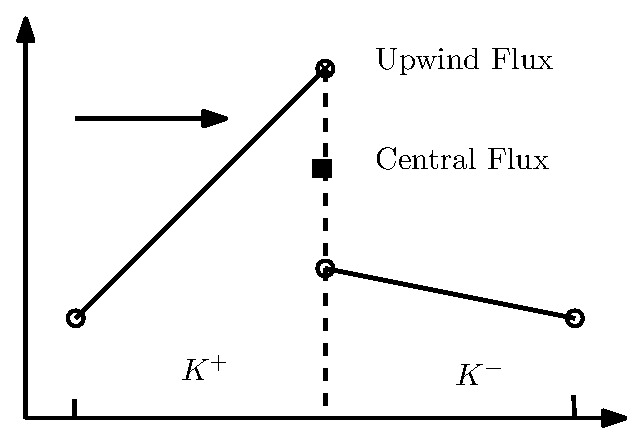
\includegraphics[width=.4\textwidth]{./FIGURES/Fig_UF_CF}
\caption{Illustration of upwind flux and central flux for one dimensional discontinuous linear functions.}\label{Fig:FLUX_CF_UF}
\end{figure}


\subsubsection{Time Stepping Method}
\label{sec:time_stepping}
In this paper, we do not focus on the time-stepping methods.   
We shall use the classical time-stepping methods to solve the following ODEs resulting from the semi-discrete DG scheme 
%
\begin{eqnarray}
   \frac{d}{dt}\mathcal{G}_h=R(\mathcal{G}_h,t)+S,
\end{eqnarray}
%
where $S$ denotes the vector term corresponding to external body source and the boundary conditions. The following implicit time stepping methods will be employed in the numerical experiments:
    \begin{eqnarray}
     \mathcal{G}_h^{n+1}&=& (\text{\bf I}-\Delta t R)^{-1}(\mathcal{G}_h^{n}+\Delta t S)
    \end{eqnarray}

In all the following tests, we will assume the time step is small enough to ensure the stability in the time discretization scheme.

\subsubsection{Pitch Angle - Collision term testing (E=R=0)}
\label{sec:pitch-angle-C}
The evolution of the pitch angle dependence of $f$ in the presence of only collisions is governed by the equation
%
\bq
\label{pitch_Coll_eq}
\frac{\partial f}{\partial t}= \frac{\partial}{\partial\xi} \left[ \left(1-\xi^2\right) \frac{\partial f}{\partial \xi} \right] \, ,
\eq
%
with initial and boundary conditions given in Eq.~(\ref{ic_bc}).
In this case the general solution is given by 
%
\bq
\label{pitch_Coll_sol}
 f(\xi, t)=\sum_{L=0}^\infty h_L P_L(\xi) e^{-L(L+1) t}\, ,
\eq
%
where $P_L$ is the Legendre polynomial of degree $L$, and the coefficients $h_L$ are determined from the initial condition according to
%
\bq
\label{pitch_Coll_ic}
 f_0(\xi)=\sum_{L=0}^\infty h_L P_L(\xi)\, .
\eq
%
\noindent{\bf Test~\ref{Subsec:Pitch-2}} 
In this test, we shall choose the initial condition as (\ref{pitch_Coll_ic}) with $L=0,\dots,6$ and $h_0=3$,  $h_1=0.5$,  $h_2=1$,  $h_3=0.7$,  $h_4=3$,  $h_6=3$.
Figure~\ref{Fig:pitch_coll}(a) plots the solution for different time periods.
%
\begin{figure}[H]
\centering
\begin{tabular}{cc}
 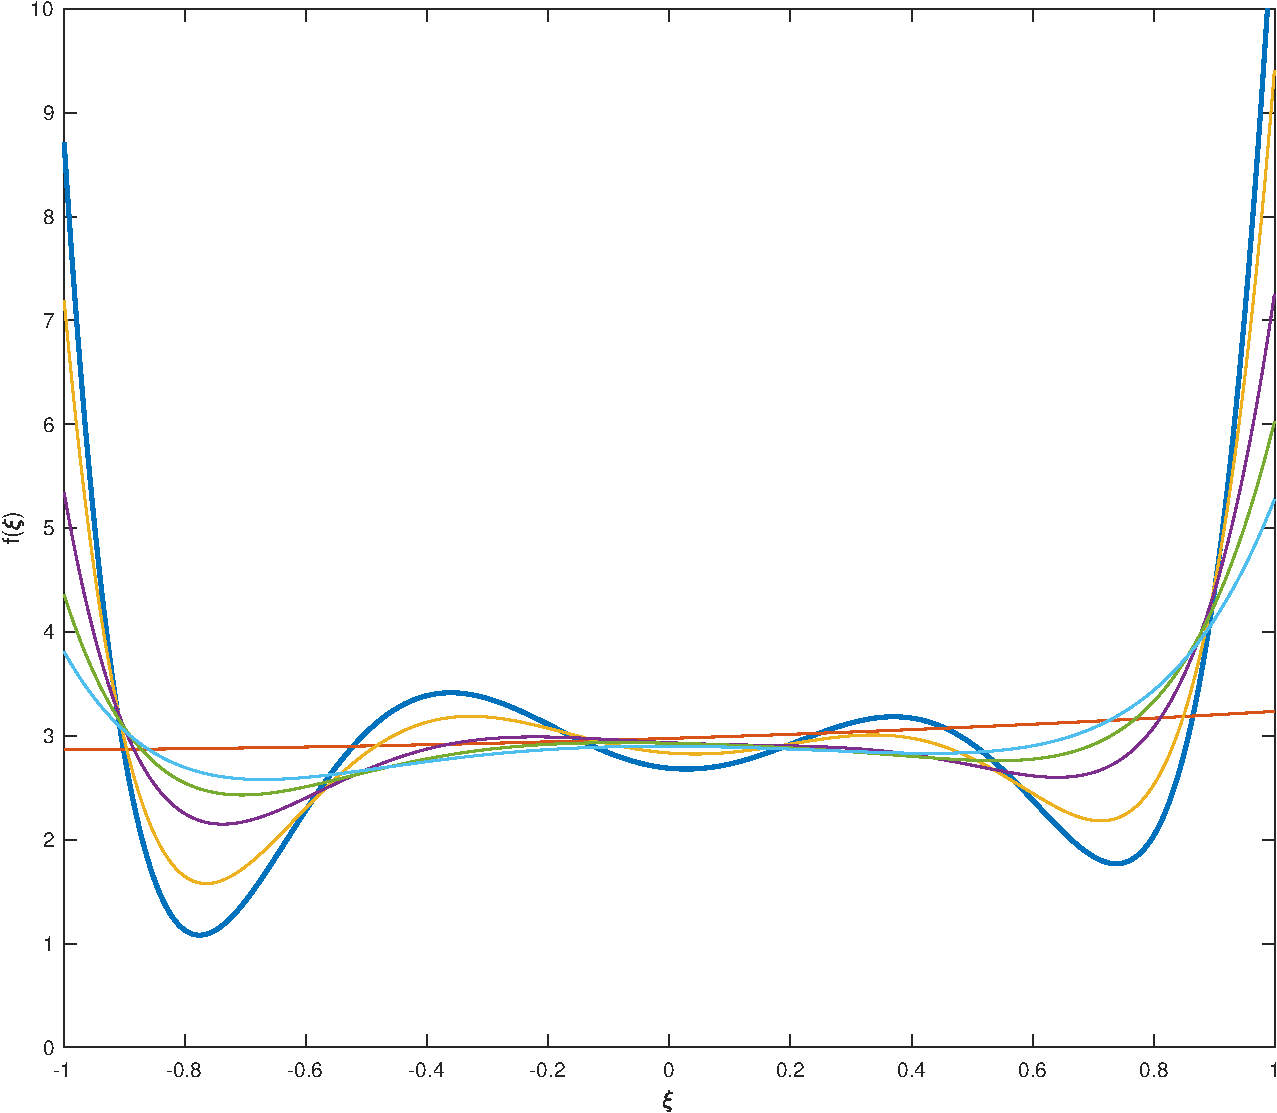
\includegraphics[width=.45\textwidth]{FIGURES/fig_Coll_time-eps-converted-to}
  &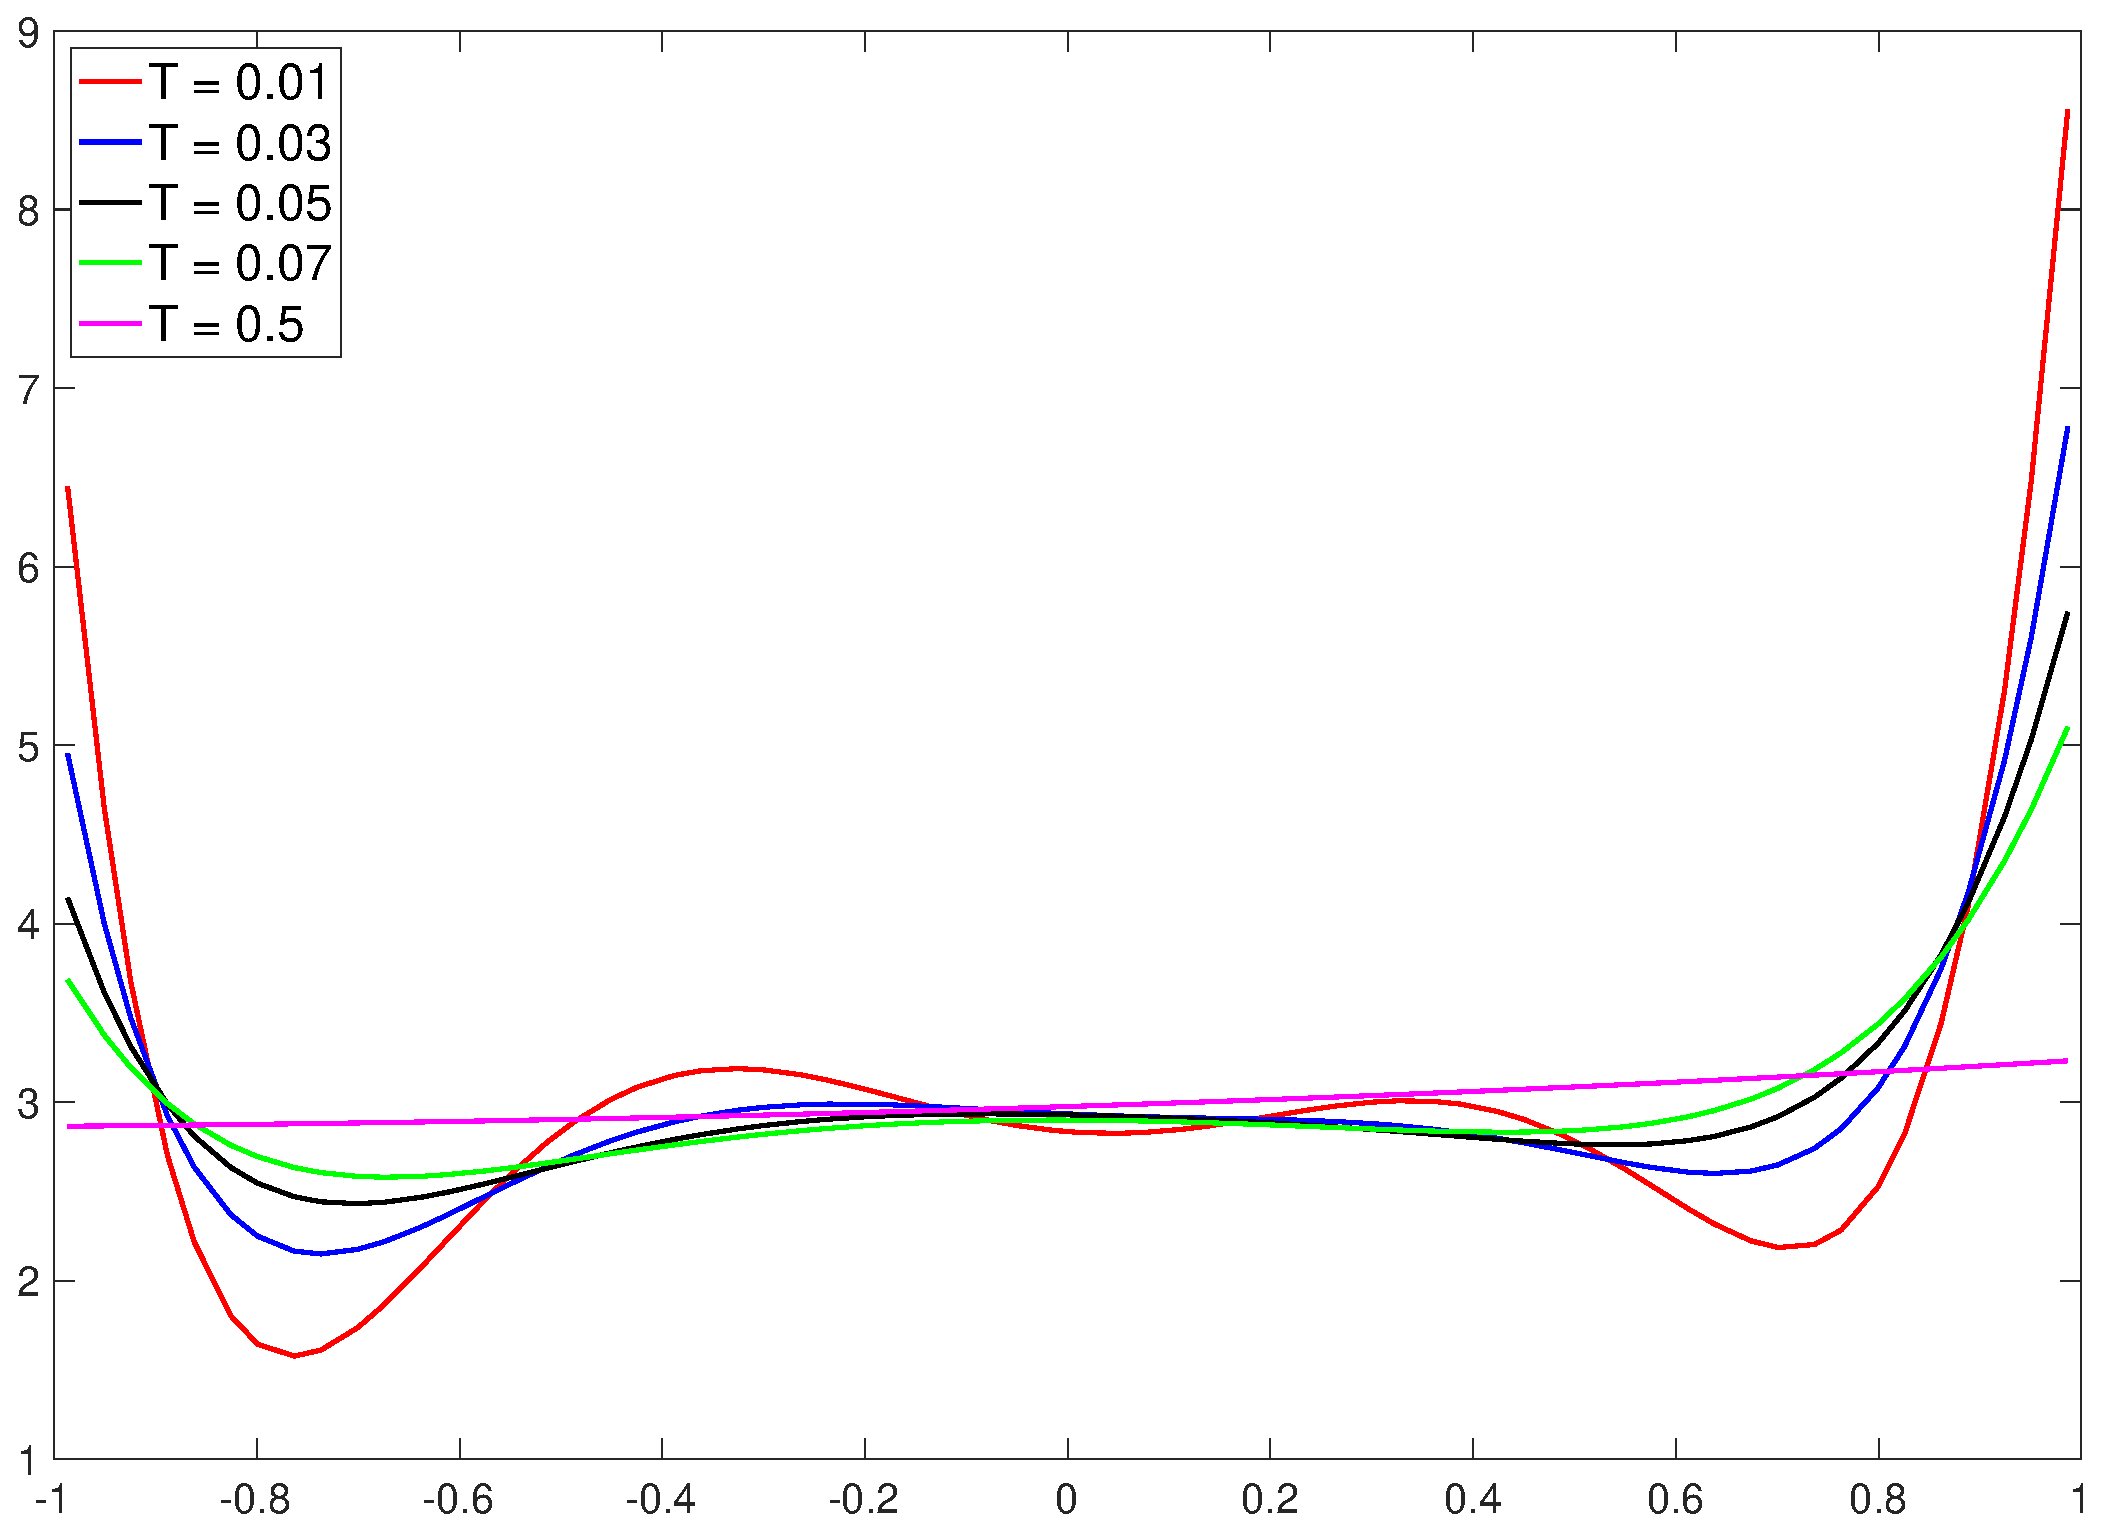
\includegraphics[width=.45\textwidth,height=.4\textwidth]{./NumFig/Diff-Deg5_Lev4}\\
  \footnotesize (a) & \footnotesize(b) 
\end{tabular}
\caption{Test~\ref{Subsec:Pitch-2}: (a) Analytical solution at 
$t=0.01$, 0.03, 0.05, 0.07 and 0.5 according to Eq.~(\ref{pitch_Coll_sol}); (b) Numerical solution with $N$ = 4 and $k$ = 5 with alternating flux.}\label{Fig:pitch_coll}
\end{figure}

The error profiles and convergence results to time period $0.03$ are reported in Table~\ref{Tab:pitch_coll}. The results show that the rate of convergence is at the order $\mathcal{O}(h^{k+1})$.
The analytical solutions and numerical solutions are plotted in Figure~\ref{Fig:pitch_coll}. As we run the simulation over longer time periods, the solution should approach a flat line, and this is validated in our numerical experiment.

{\small
\begin{table}[H]
\caption{Test~\ref{Subsec:Pitch-2}: Error profiles and convergence test of time = $0.03$ for alternating flux.}\label{Tab:pitch_coll}
\centering
\begin{tabular}{c|cc|cc}	\hline\hline
$N$ & $\|f-f_h\|_{\infty}$ & Rate & $\|f-f_h\|$ & Rate \\ \hline		
&\multicolumn{4}{c}{$k=1$}\\ \hline
2	&4.7098E-01	&	&2.0224E-01	&\\
3	&4.3233E-01	&0.12	&1.4733E-01	&0.46\\
4	&1.6836E-01	&1.36	&5.2630E-02	&1.49\\
5	&4.8070E-02	&1.81	&1.4376E-02	&1.87\\
6	&1.2284E-02	&1.97	&3.6140E-03	&1.99\\
7	&3.0468E-03	&2.01	&8.9771E-04	&2.01\\ \hline		
&\multicolumn{4}{c}{$k=2$}\\ \hline
2	&1.8990E-01	&	&1.0574E-01 &	\\
3	&5.4641E-02	&1.80	&2.4824E-02	&2.09\\
4	&9.7264E-03	&2.49	&3.3980E-03	&2.87\\
5	&1.2774E-03	&2.93	&4.1204E-04	&3.04\\
6	&1.5756E-04	&3.02	&5.0447E-05	&3.03\\
7	&1.9595E-05	&3.01	&6.2620E-06	&3.01\\ \hline		
&\multicolumn{4}{c}{$k=3$}\\ \hline
2	&3.8318E-02	&	&2.2665E-02	&\\
3	&3.8223E-03	&3.33	&1.7168E-03	&3.72\\
4	&2.6078E-04	&3.87	&1.0377E-04	&4.05\\
5	&1.6003E-05	&4.03	&6.3061E-06	&4.04\\
6	&9.8794E-07	&4.02	&3.9057E-07	&4.01\\
7	&6.1477E-08	&4.01	&2.4346E-08	&4.00\\ \hline\hline
\end{tabular}
\end{table}
}


\subsubsection{Pitch Angle - Electric field acceleration term testing (C=R=0)}
\label{Subsec:Pitch-1}
The evolution of the pitch angle dependence of $f$ in the presence of only electric field acceleration is governed by the equation
%
\bq
\label{pitch_E_eq}
\frac{\partial f}{\partial t}= - \frac{\partial}{\partial\xi} \left[ \left(1-\xi^2\right) f \right] \, ,
\eq
%
with
%
\bq
\label{ic_bc}
f(\xi, t=0)=f_0(\xi)\, , \qquad (1-\xi^2)f|_{\xi=\pm 1}=0 \, ,
\eq
%
where $f_0(\xi)$ is the initial condition. The general analytical solution of this problem is
%
\bq
\label{pitch_E_sol}
f(\xi,t)=\left[ \frac{1-\phi^2}{1-\xi^2}\right]\, f_0(\phi)\, , \qquad \phi=\tanh \left( \tanh^{-1} \xi -t \right) \, .
\eq

\noindent{\bf Test~\ref{Subsec:Pitch-1}a} First we set the initial condition as $f_0=1$ and the solution is plotted in Figure~\ref{Fig:Pitch_E_1}. 
It is noted that, as shown in the figure, the solution asymptotically approaches a Dirac delta function centered at $\xi=1$. 
\todo{TY: Based on my attempted verification, these results are using downwind flux. By Lin: This is Hyperbolic equation. Does downwind work?}
%
\begin{figure}[H]
\centering
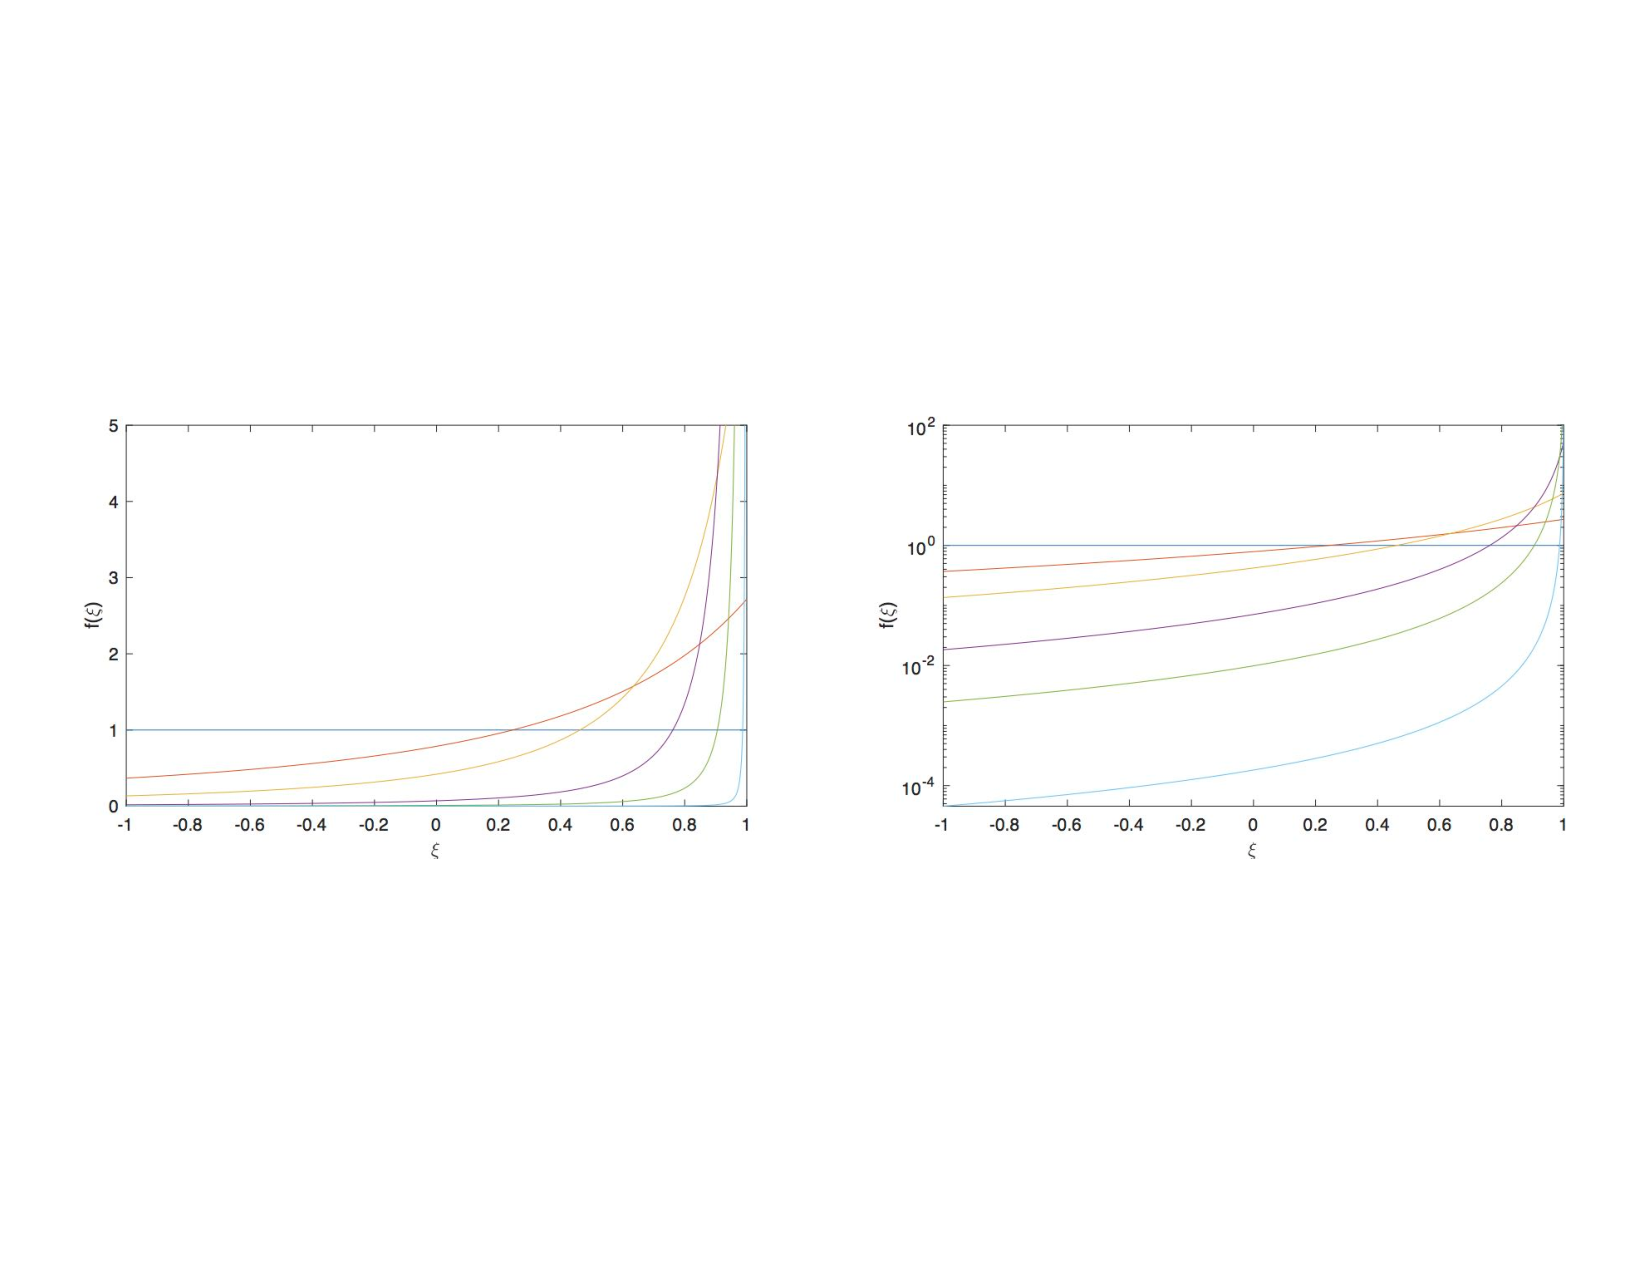
\includegraphics[scale=0.5]{FIGURES/fig_E_pitch}
\caption{Test~\ref{Subsec:Pitch-1}a. Analytical solution of Eq.~(\ref{pitch_E_eq}) at 
$t=0$. 0.5, 1, 2 and 3 according to Eq.~(\ref{pitch_E_sol}) for initial condition $f_0=1$. Left figure plot the solution; right figure illustrates the semiloy plot of the solution.}\label{Fig:Pitch_E_1}
\end{figure}

{\small
\begin{table}[H]
\caption{Test~\ref{Subsec:Pitch-1}a: Error profiles and convergence test by central flux (denoted as CF) and upwind flux (denoted as UF).}\label{Tab:Pitch_E-1}
\centering
\begin{tabular}{c|cc|cc}	\hline\hline
& \multicolumn{2}{c|}{CF} &\multicolumn{2}{c}{UF}\\ \hline
$N$ & $\|f-f_h\|$ & Rate & $\|f-f_h\|$ & Rate \\ \hline		
&\multicolumn{4}{c}{$k=1$}\\ \hline
3	&1.5842E-01	&	        &3.4551E-02	& \\
4	&7.8928E-02	&1.01	&1.4192E-02	&1.28\\
5	&3.9003E-02	&1.02	&5.4647E-03	&1.38\\
6	&1.9405E-02	&1.01	&1.8316E-03	&1.58\\
7	&9.6866E-03	&1.00	&5.5644E-04	&1.72\\ \hline
			&\multicolumn{4}{c}{$k=2$}\\ \hline	
3	&1.5096E-02	&	&5.0869E-03	& \\
4	&1.9768E-03	&2.93	&1.0561E-03	&2.27\\
5	&1.7549E-04	&3.49	&2.3978E-04	&2.14\\
6	&1.2671E-05	&3.79	&4.4522E-05	&2.43\\
7	&8.4519E-07	&3.91	&7.1143E-06	&2.65\\ \hline
			&\multicolumn{4}{c}{$k=3$}\\ \hline	
3	&4.2329E-03	&	&8.0931E-04	& \\
4	&5.9217E-04	&2.84	&8.2762E-05	&3.29\\ 
5	&7.4760E-05	&2.99	&1.0673E-05	&2.96\\
6	&9.2476E-06	&3.02	&1.0853E-06	&3.30\\ 
7	&1.1471E-06	&3.01	&9.0918E-08	&3.58\\ \hline\hline
\end{tabular}
\end{table}
}

\begin{figure}[H]
\begin{tabular}{cc}
  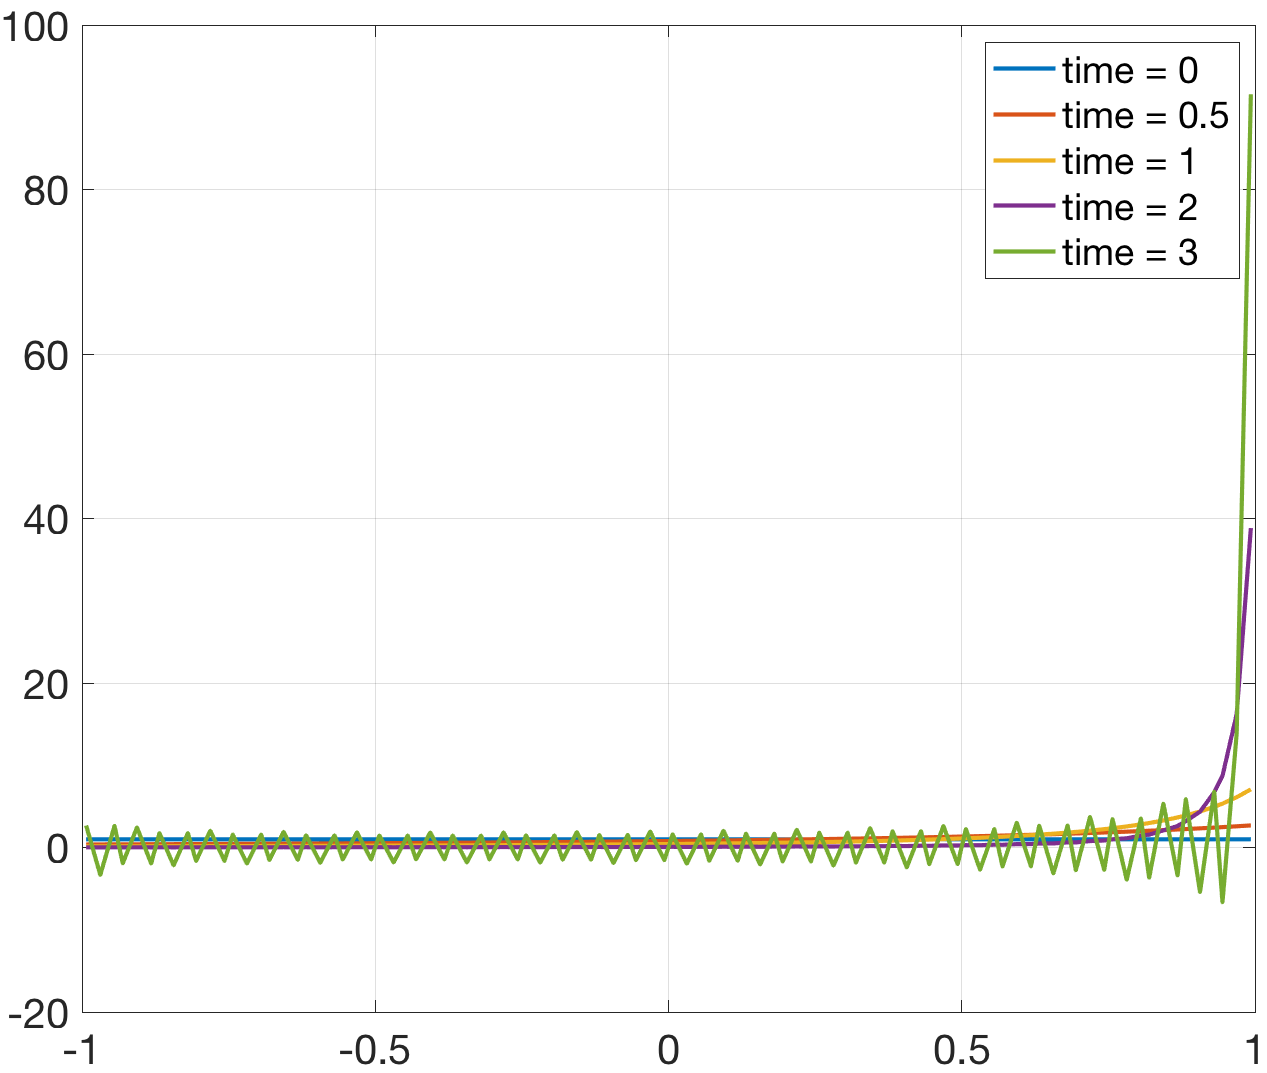
\includegraphics[width=.45\textwidth,height=.3\textwidth]{./NumFig/Test1-CF-L5D5}
  &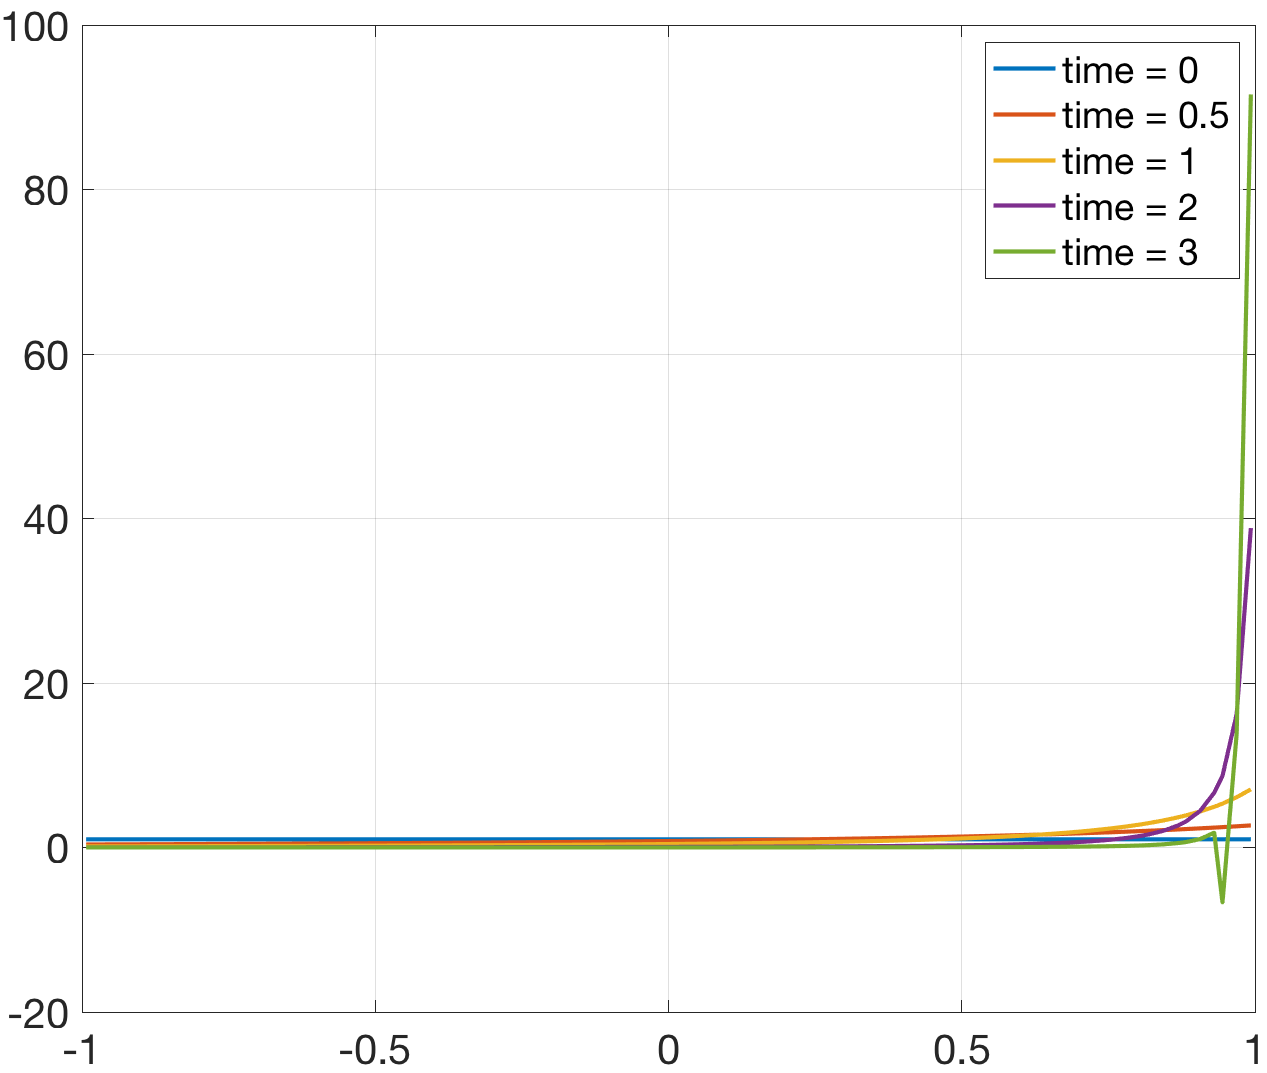
\includegraphics[width=.45\textwidth,height=.3\textwidth]{./NumFig/Test1-UF-L5D5}\\
  (a) & (b)
  \end{tabular}
  \caption{Test~\ref{Subsec:Pitch-1}a. Plot for numerical solutions for maximum Level $N=5$, $k = 4$ at $t = $ 0.5, 1, 2, 3 with (a) central flux; (b) upwind flux.}\label{Fig:Pitch_E_1-Num2}
\end{figure}

The error profiles and convergence results are reported in Table~\ref{Tab:Pitch_E-1}. One can observe that $L^2$-error converges at the order $\mathcal{O}(h^k)$ for central flux if $k$ is odd. In the case of employing $k=2$, we obtain super-convergence with rate around $\mathcal{O}(h^{k+1})$. By employing upwind flux, one can observe convergence rate $\mathcal{O}(h^{k+1/2})$, which is half order higher than that of using central flux for odd $k$. 

Numerical experiments have been carried out on the mesh with $N = 5$, $k = 4$, and the numerical solutions are plotted in Figure~\ref{Fig:Pitch_E_1-Num2} for central flux and upwind flux. Since the solution approaches a Dirac delta function centered at $\xi$, the numerical solution cannot capture the analytical solutions on the right end point after several time steps. Thus, one begins to observe oscillations in the plot for both fluxes. Though the upwind flux cannot provide an oscillation-free scheme, the undershoots are around coordinate $1$. By using center flux, however, the numerical solution is oscillating in the whole domain. This test shows the advantage of upwind flux.

\vskip.1in
\noindent{\bf Test~\ref{Subsec:Pitch-1}b} In this test, we set the initial condition as $f_0=\exp (-\xi^2/\sigma^2)$ with $\sigma=0.1$ and the solution is plotted in Figure~\ref{Fig:Pitch_E_2}. It is noted that, as shown in the figure, the solution asymptotically approaches a Dirac delta function centered at $\xi=1$.

\begin{figure}[H]
\centering
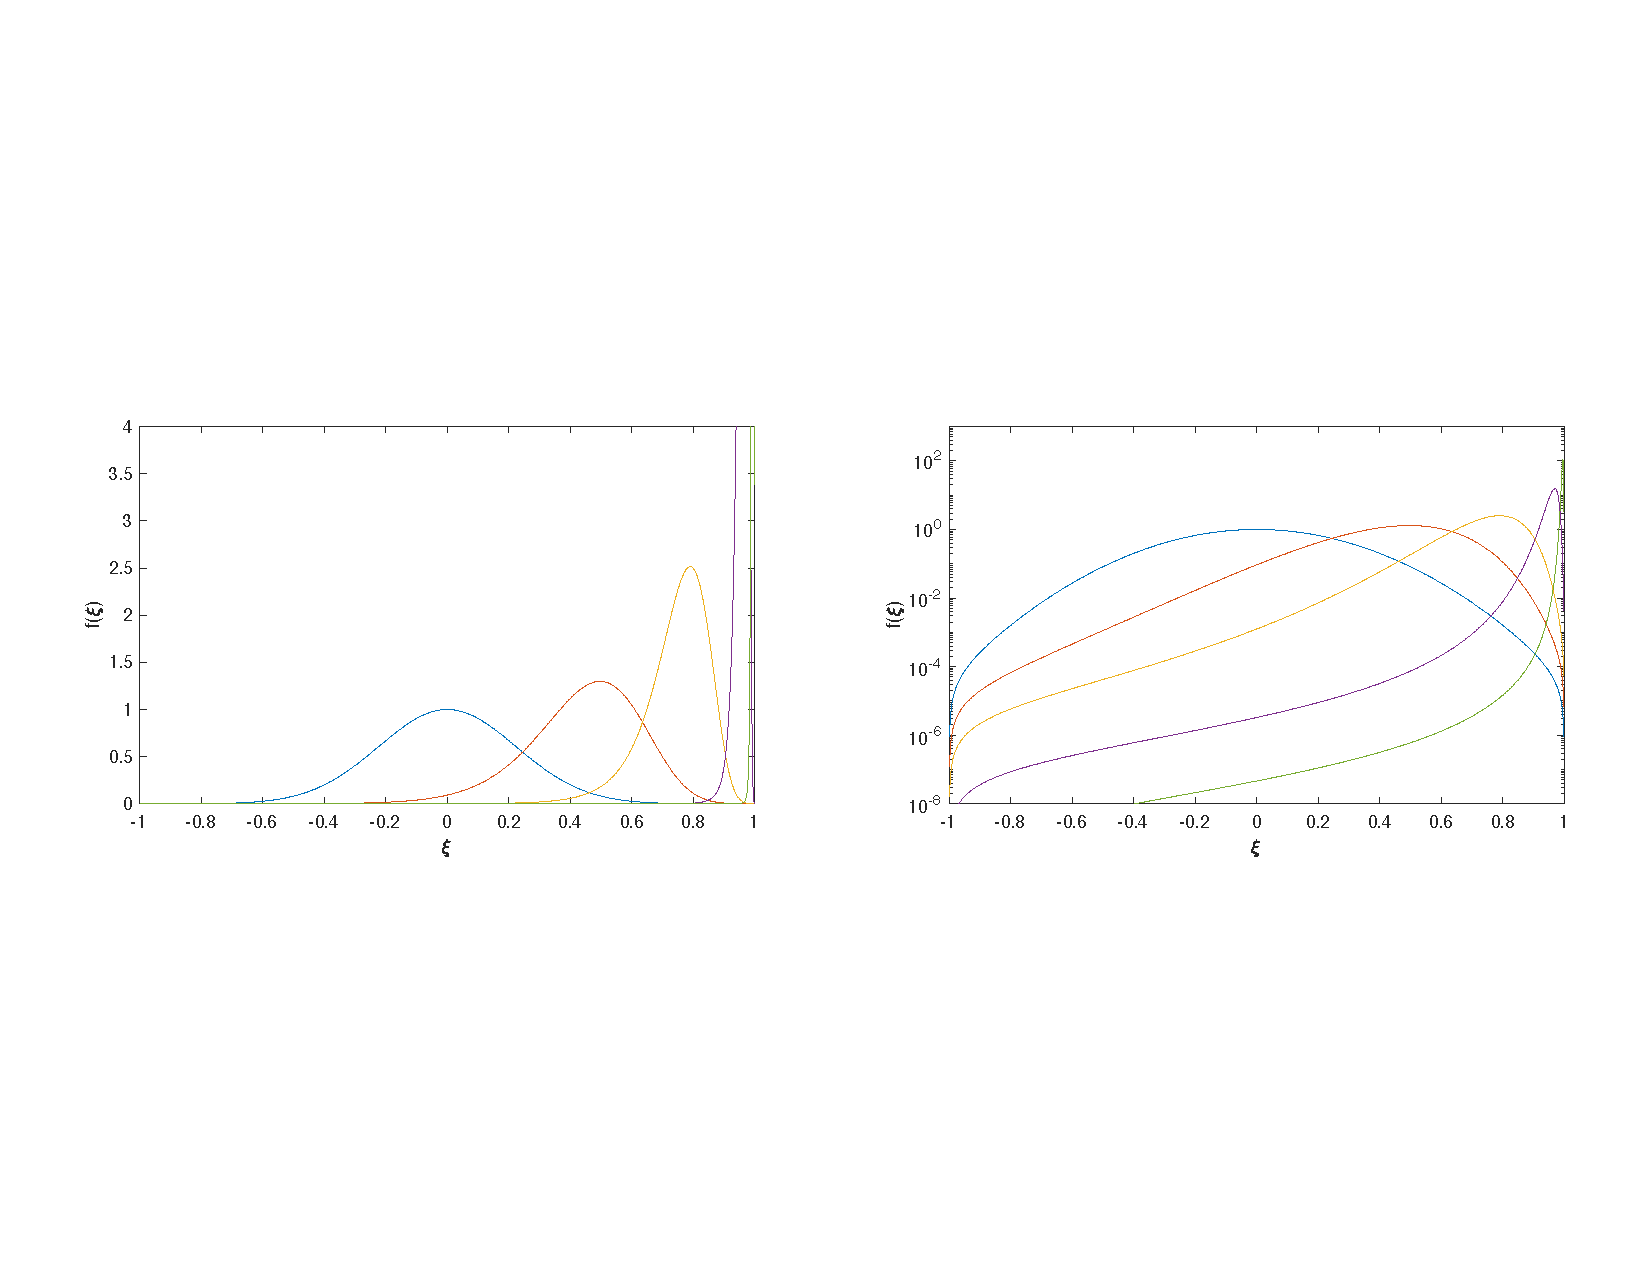
\includegraphics[scale=0.5]{FIGURES/fig_E_pitch_Gaussian}
%\label{fig_pitch_E_2}
\caption{Test~\ref{Subsec:Pitch-1}b. Analytical solution of Eq.~(\ref{pitch_E_eq}) at 
$t=0$, 0.5, 1, 2 and 3 according to Eq.~(\ref{pitch_E_sol}) for initial condition $f_0=\exp(-\xi^2/\sigma^2)$. Left figure plot the solution; right figure illustrates the semiloy plot of the solution.}\label{Fig:Pitch_E_2}
\end{figure}
%
\begin{figure}[H]
\centering
\begin{tabular}{cc}
  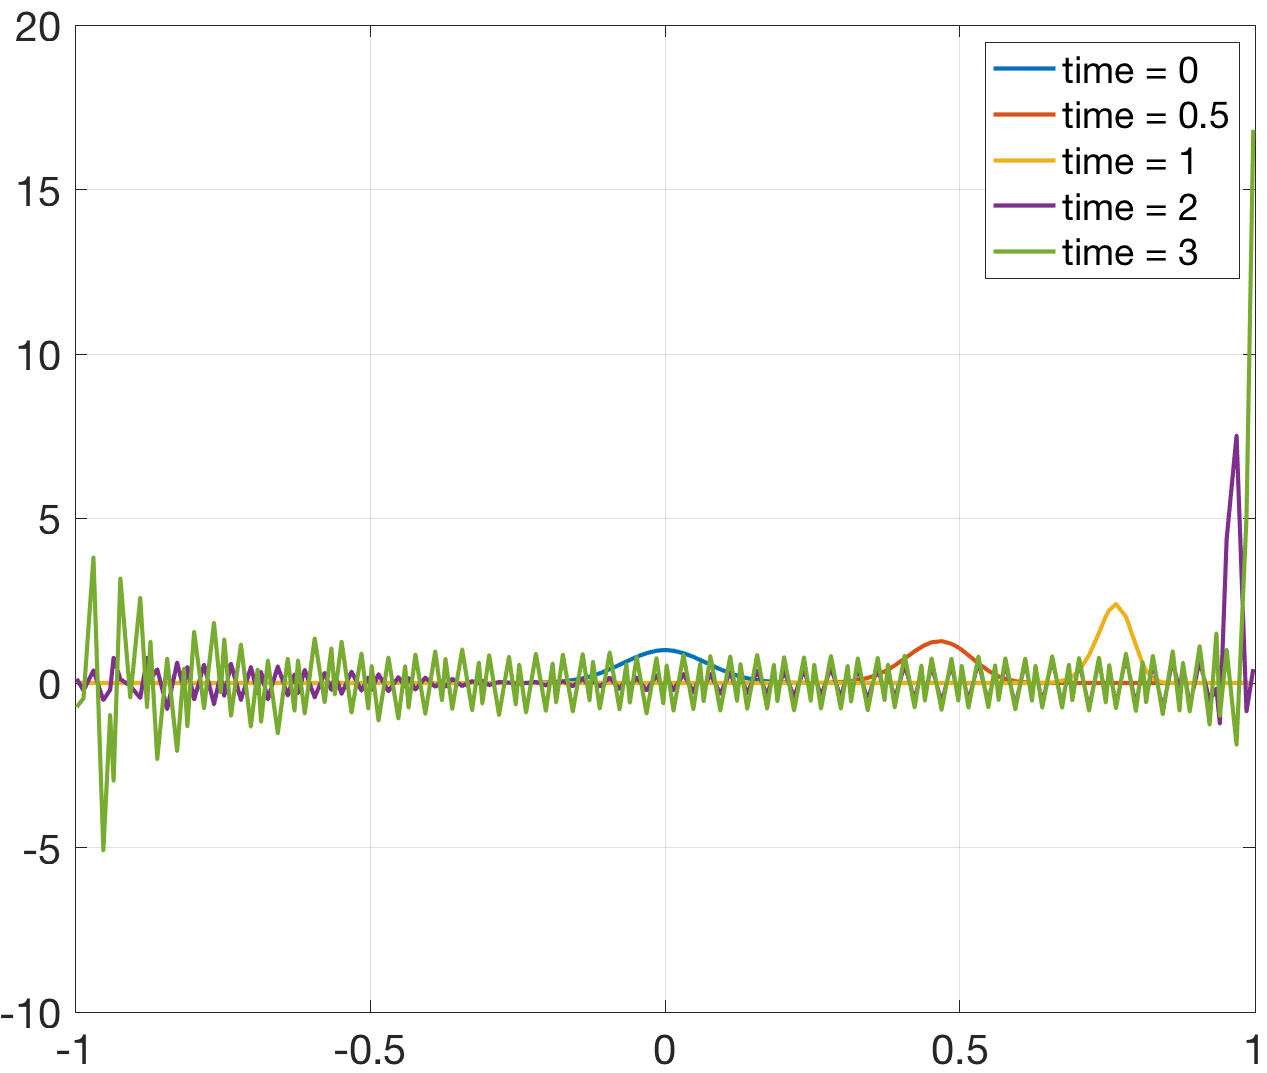
\includegraphics[width=.4\textwidth]{./NumFig/Test1-2-CF-L5D5}
  &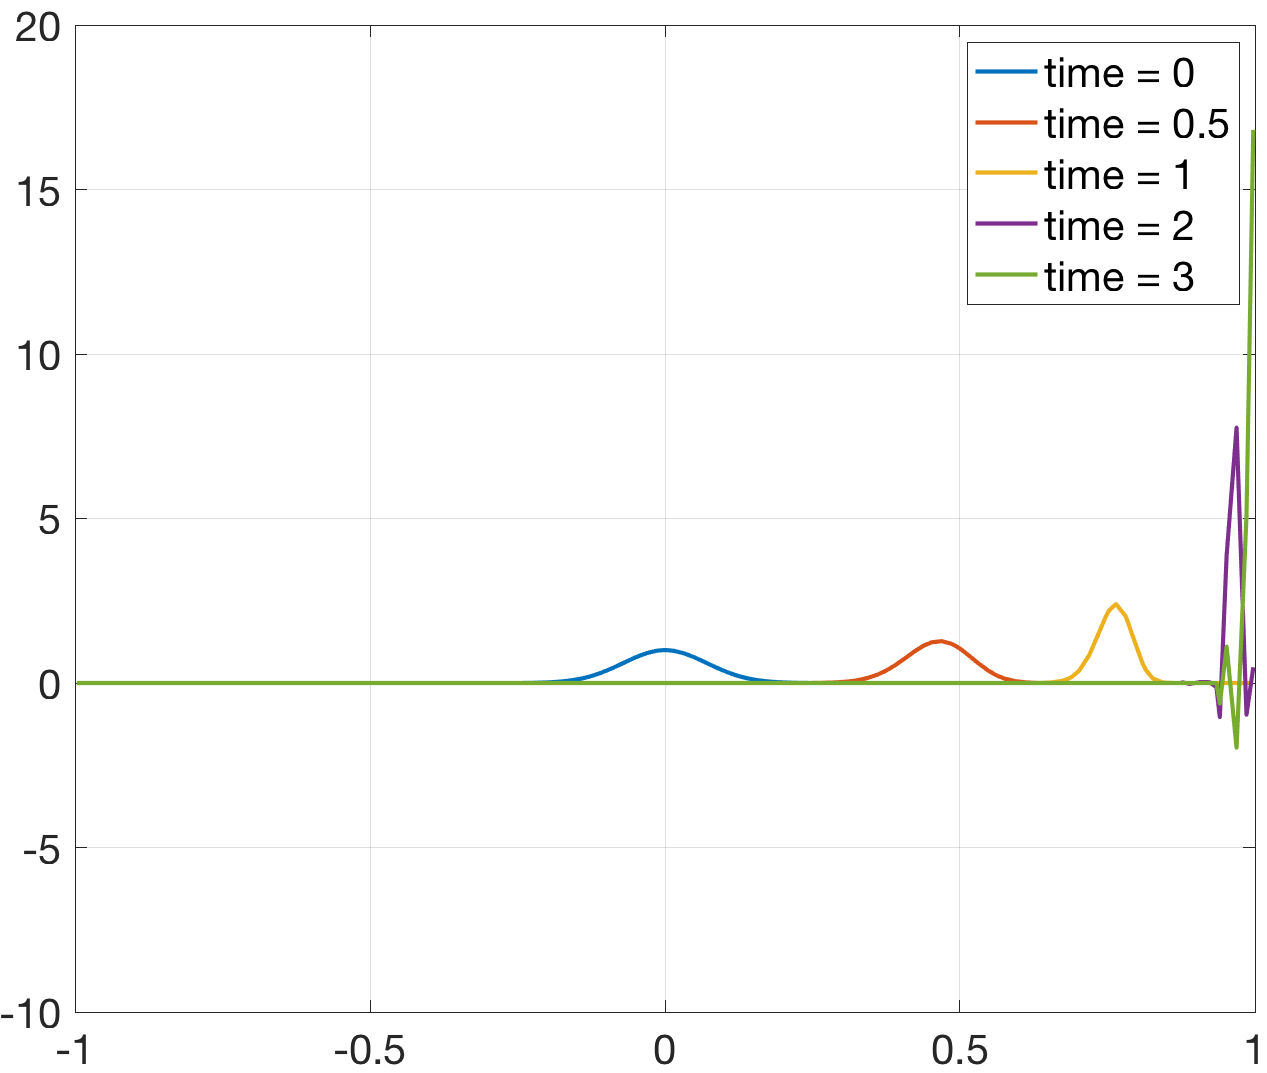
\includegraphics[width=.4\textwidth]{./NumFig/Test1-2-UF-L5D5}\\
  (a) & (b)
  \end{tabular}
  \caption{Test~\ref{Subsec:Pitch-1}b. Plot for numerical solutions for $N=5$, $k = 4$ at $t = $ 0.5, 1, 2, 3: (a) central flux; (b) upwind flux.}\label{Fig:Pitch_E_2-Num2}
\end{figure}
%
The numerical experiment has been carried out on the mesh with $N$ = 5, $k = 4$, and the numerical solutions are plotted in Figure~\ref{Fig:Pitch_E_2-Num2} for central flux and upwind flux. Similar conclusion regarding the upwind flux and central flux can be made for this test.


\subsubsection{Pitch Angle - Radiation damping term testing (C=E=0)}
\label{Subsec:Pitch-3}
The evolution of the pitch angle dependence of $f$ in the presence of only radiation damping is governed by the equation
%
\bq
\label{pitch_Rad_eq}
\frac{\partial f}{\partial t}= -\frac{\partial}{\partial\xi} \left[\xi \left(1-\xi^2\right) f\right] \, ,
\eq
%
with initial and boundary conditions given in Eq.~(\ref{ic_bc}).
In this case the general solution is given by 
%
\bq
\label{pitch_Rad_sol}
f(\xi,t)=\frac{\phi \left ( 1- \phi^2\right)}{\xi \left(1-\xi^2\right)}\, f_0(\phi) \, ,
\eq
%
where
%
\bq
\phi=\frac{\xi e^{-t}}{\sqrt{1+\left(e^{-2t}-1\right) \xi^2}}\, .
\eq
%
\noindent{\bf Test~\ref{Subsec:Pitch-3}} In this test, we shall set the function $f_0$ to different Gaussian functions:
\begin{eqnarray}
\text{Case 1.   }f_0 &=& \exp(-\frac{\xi^2}{\sigma^2}),\\
\text{Case 2.   }f_0 &=& \exp(-\frac{(\xi-0.36)^2}{\sigma^2}),\\
\text{Case 3.   }f_0 &=& \exp(-\frac{(\xi+0.36)^2}{\sigma^2}),\\
\text{Case 4.   }f_0 &=& \exp(-\frac{(\xi-0.36)^2}{\sigma^2})+\exp(-\frac{(\xi+0.36)^2}{\sigma^2}).
\end{eqnarray}

We perform the proposed numerical scheme in the simulation and the numerical results for Case 1 are reported in Table~\ref{Tab:pitch_rad}. It shows that error, measured in $\|\cdot\|_{\infty}$ and $\|\cdot\|$-norms, converges at the order $\mathcal{O}(h^{k+1})$. One can also observe super-convergence for $k=2$.

\begin{table}[H]
\caption{Test~\ref{Subsec:Pitch-3} (Case 1): Error profiles and convergence test with upwind flux at time$=3$.}\label{Tab:pitch_rad}
\centering
\begin{tabular}{c|cc|cc}	\hline\hline
$N$ & $\|f-f_h\|_{\infty}$ & Rate & $\|f-f_h\|$ & Rate \\ \hline		
&\multicolumn{4}{c}{$k=1$}\\ \hline
3	&3.9497E-02	&	&2.3490E-02	& \\
4	&1.8914E-02	&1.06	&9.0040E-03	&1.38\\
5	&1.0083E-02	&0.91	&2.7059E-03	&1.73\\
6	&3.1273E-03	&1.69	&5.0826E-04	&2.41\\
7	&8.2423E-04	&1.92	&9.5484E-05	&2.41\\
8	&2.0879E-04	&1.98	&1.8460E-05	&2.37\\ \hline
	&\multicolumn{4}{c}{$k=2$}\\ \hline			
3	&2.5594E-02	&	&1.2153E-02	& \\
4	&1.0656E-02	&1.26	&3.3830E-03	&1.84\\
5	&1.1431E-03	&3.22	&3.1490E-04	&3.43\\
6	&8.2237E-05	&3.80	&2.6488E-05	&3.57\\
7	&6.6415E-06	&3.63	&1.7363E-06	&3.93\\
8	&4.8922E-07	&3.76	&1.0024E-07	&4.11\\ \hline
		&\multicolumn{4}{c}{$k=3$}\\ \hline		
3	&1.7571E-02	&	&7.5736E-03	& \\
4	&4.2588E-04	&5.37	&1.8950E-04	&5.32\\
5	&1.2814E-04	&1.73	&3.0874E-05	&2.62\\
6	&1.1815E-05	&3.44	&2.0460E-06	&3.92\\
7	&8.0768E-07	&3.87	&1.1012E-07	&4.22\\
8	&5.1717E-08	&3.97	&6.0220E-09	&4.19\\ \hline\hline
\end{tabular}
\end{table}

Then, we test our numerical scheme on the mesh with $N=8$ and $k=1$ and the numerical solutions are plotted in Figure~\ref{Fig:Pitch-3-1}-\ref{Fig:Pitch-3-4}. As shown in these figure, it is noted that our numerical scheme preserves total mass very well throughout all the computations.

\begin{figure}[H]
\centering
\begin{tabular}{ccc}
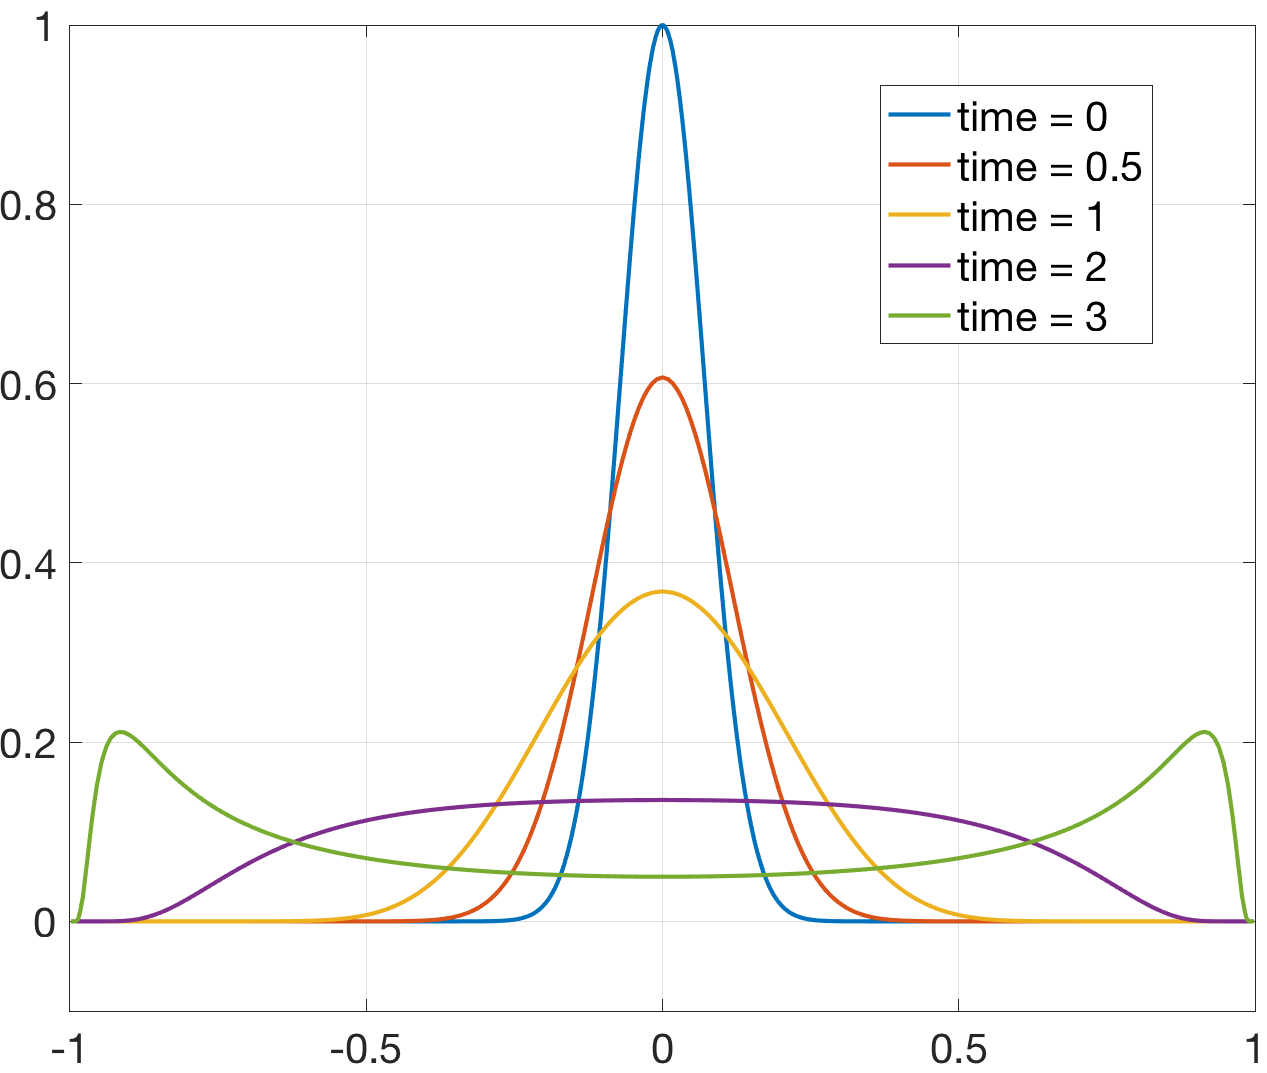
\includegraphics[width=.3\textwidth]{./NumFig/Test4-3-1-L8D2}
&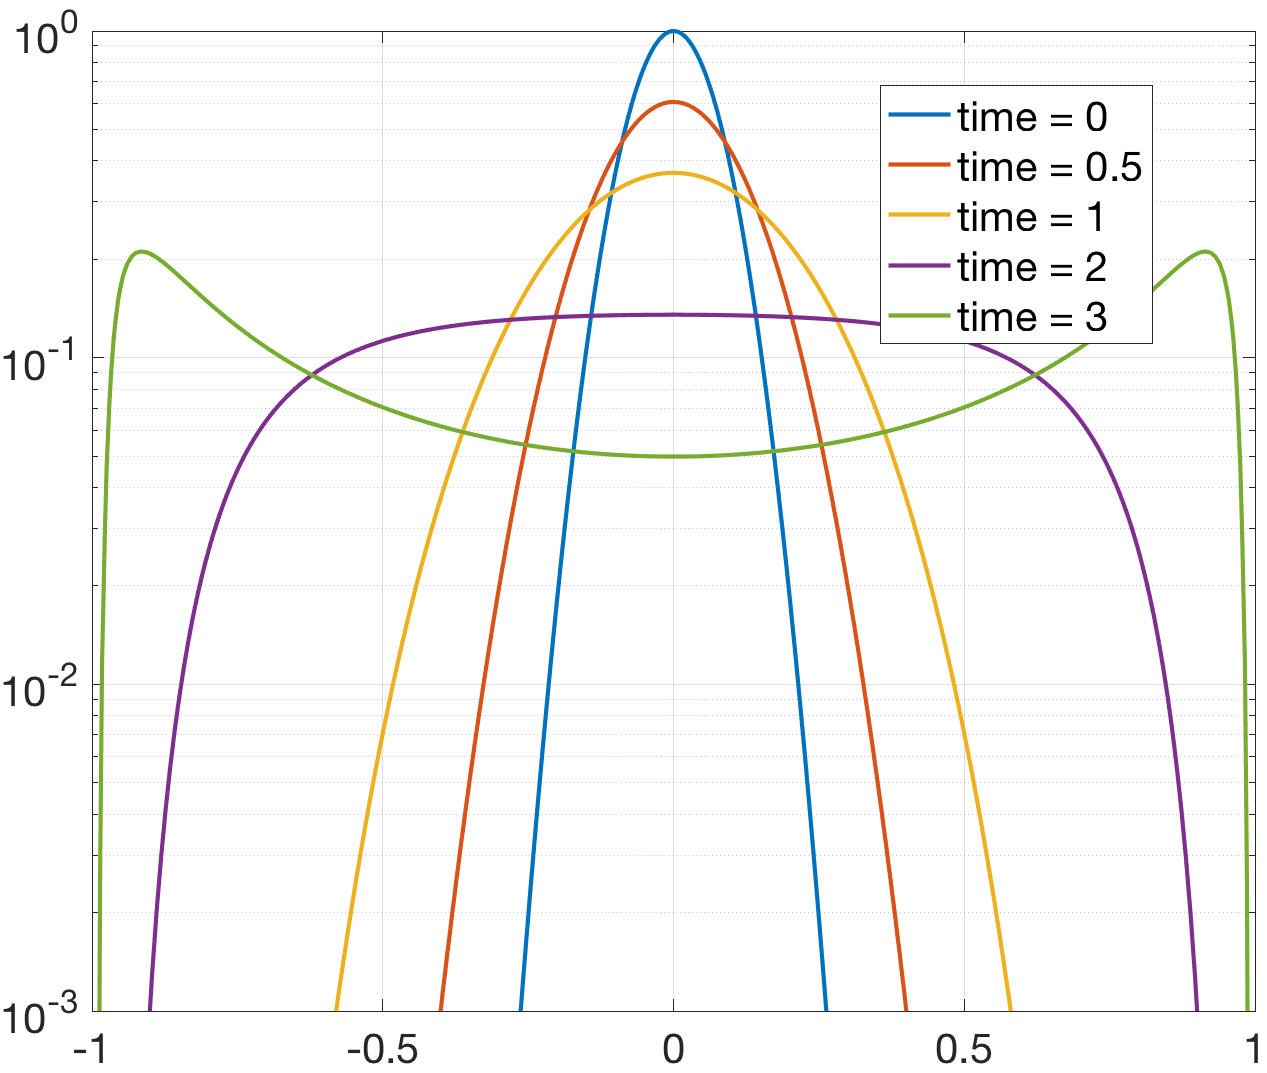
\includegraphics[width=.3\textwidth]{./NumFig/Test4-3-1-L8D2-log}
&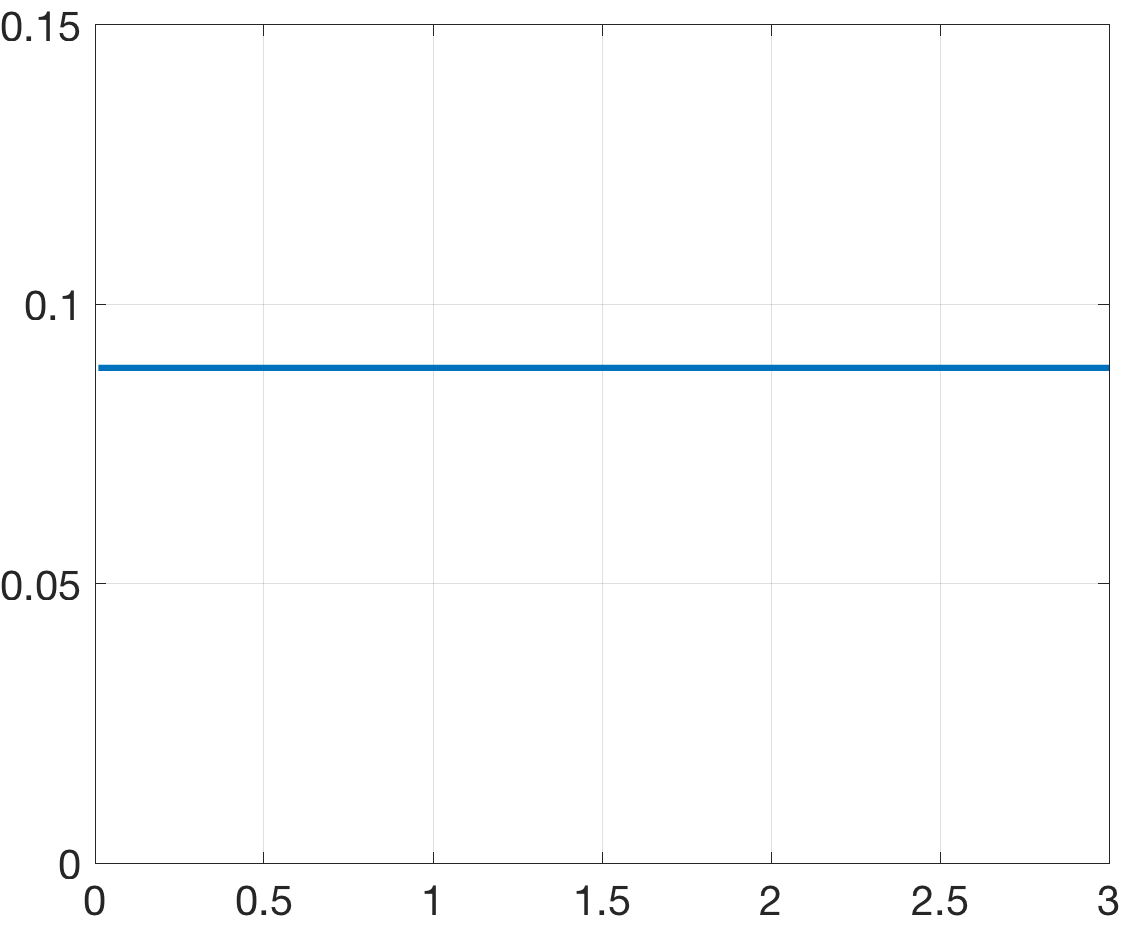
\includegraphics[width=.3\textwidth]{./NumFig/Test4-3-k1-1-Con_v2}\\
(a) & (b) &(c)
\end{tabular}
\caption{Test~\ref{Subsec:Pitch-3} (case 1): Plots of numerical solutions at time $=0,0.5,1,2,3$ on mesh with $N$ = 8, $k=1$: (a) Plot of numerical solutions; (b) semilog plot of numerical solutions; (c) plot of total mass.}\label{Fig:Pitch-3-1}
\end{figure}

\begin{figure}[H]
\centering
\begin{tabular}{ccc}
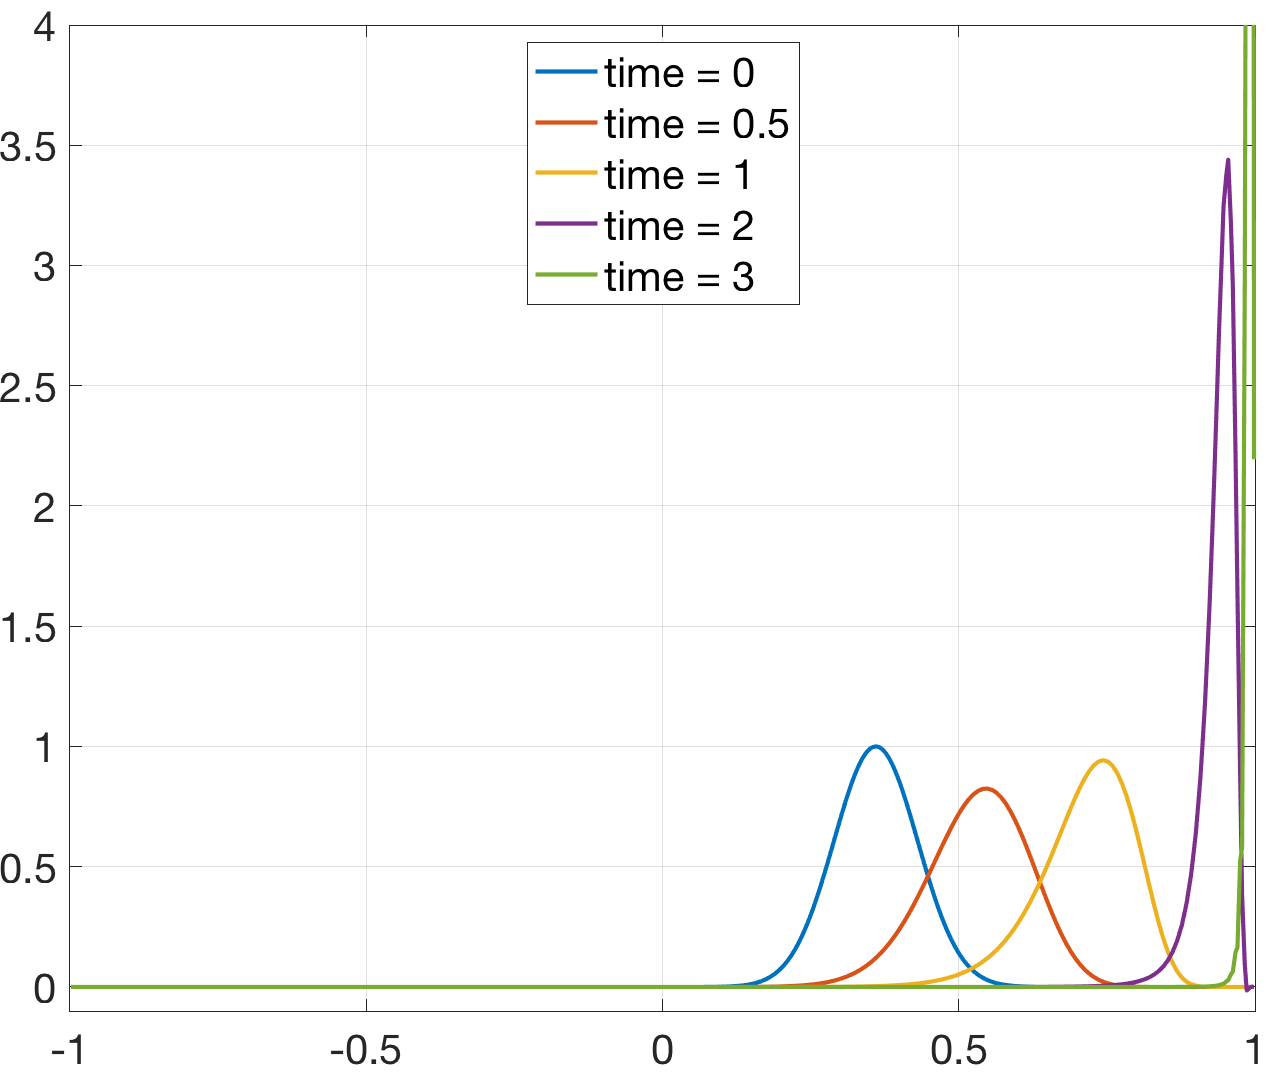
\includegraphics[width=.3\textwidth]{./NumFig/Test4-3-3-L8D2}
&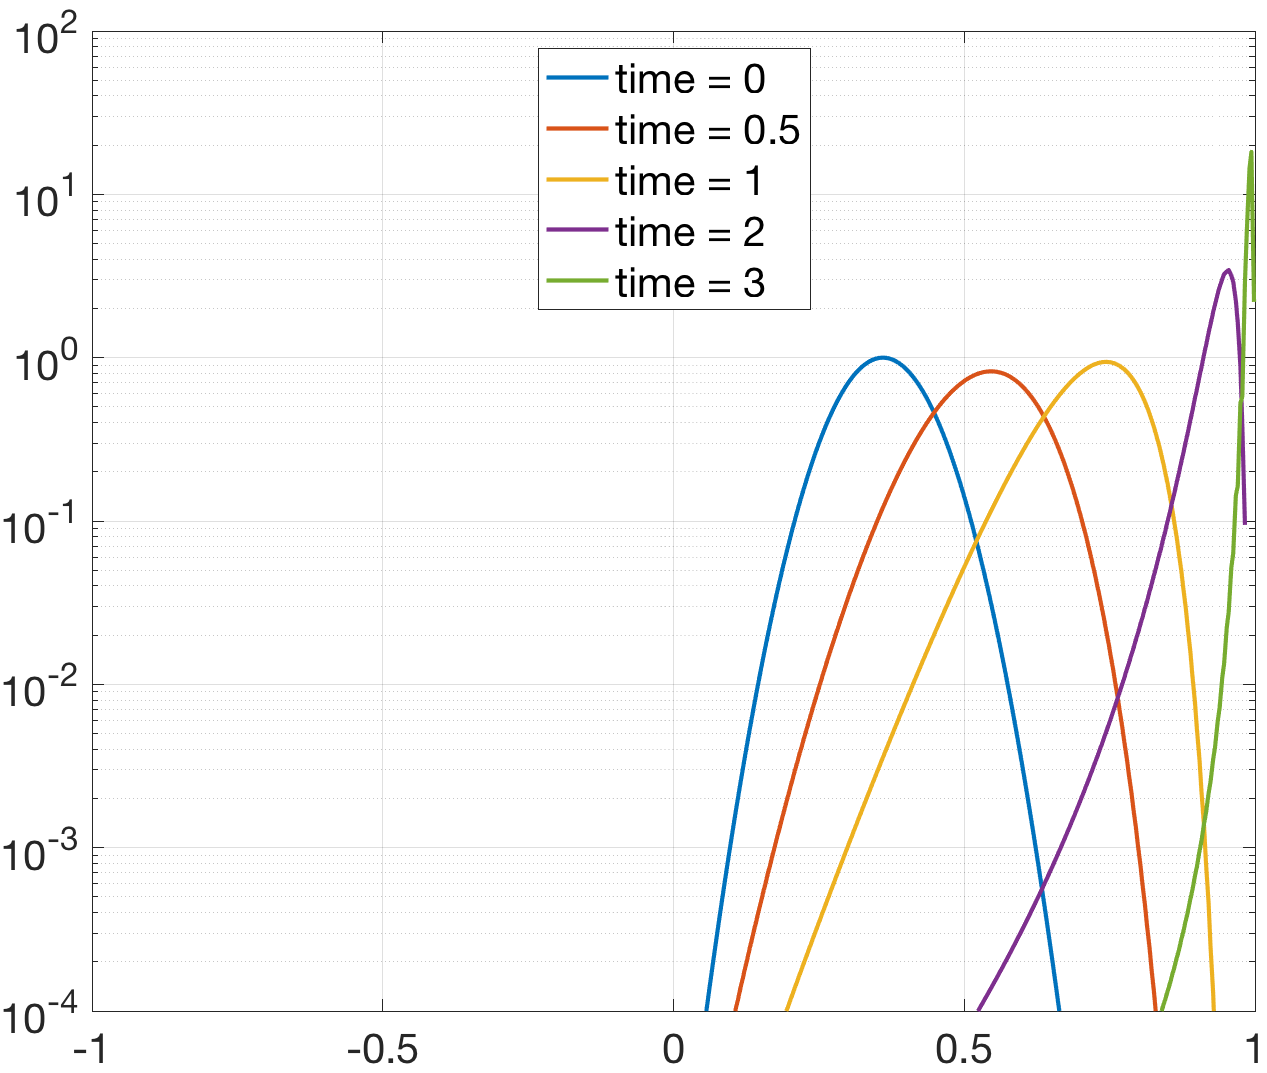
\includegraphics[width=.3\textwidth]{./NumFig/Test4-3-3-L8D2-log}
&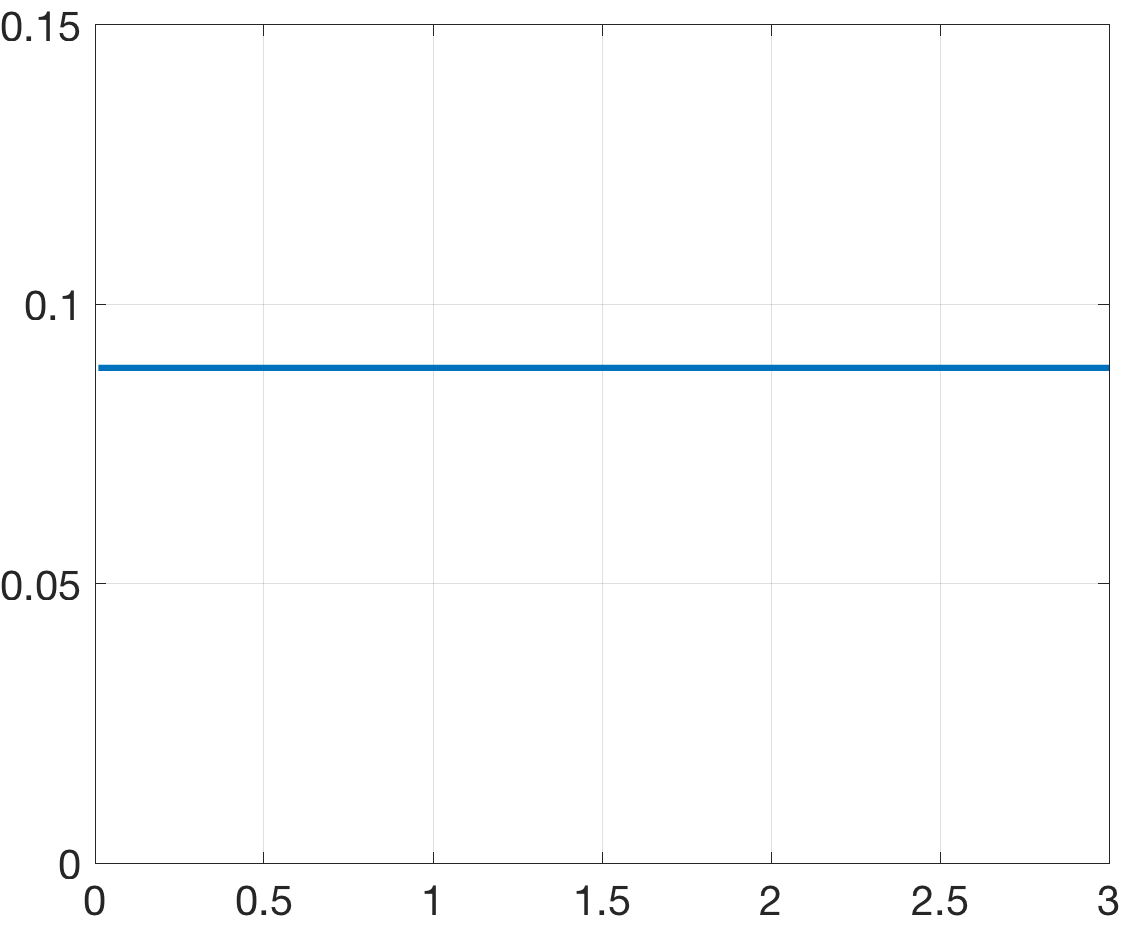
\includegraphics[width=.3\textwidth]{./NumFig/Test4-3-k1-3-Con_v2}
\\
(a) & (b) &(c)
\end{tabular}
\caption{Test~\ref{Subsec:Pitch-3} (case 2): Plots of numerical solutions at time $=0,0.5,1,2,3$ on mesh with $N$ = 8, $k=1$: (a) Plot of numerical solutions; (b) semilog plot of numerical solutions; (c) plot of total mass.}\label{Fig:Pitch-3-2}
\end{figure}

\begin{figure}[H]
\centering
\begin{tabular}{ccc}
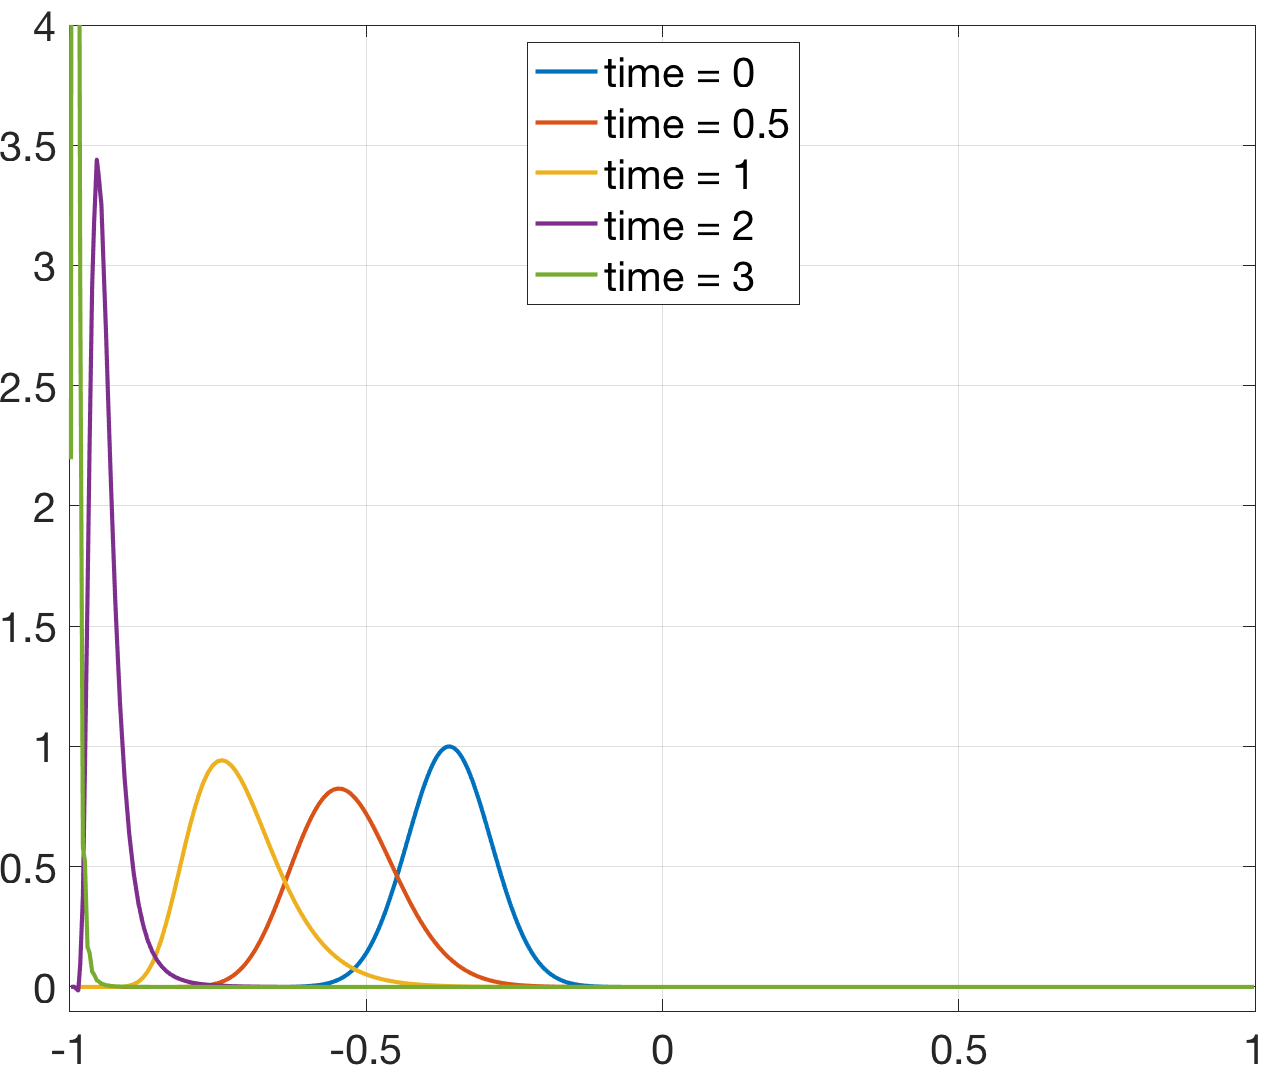
\includegraphics[width=.3\textwidth]{./NumFig/Test4-3-2-L8D2}
&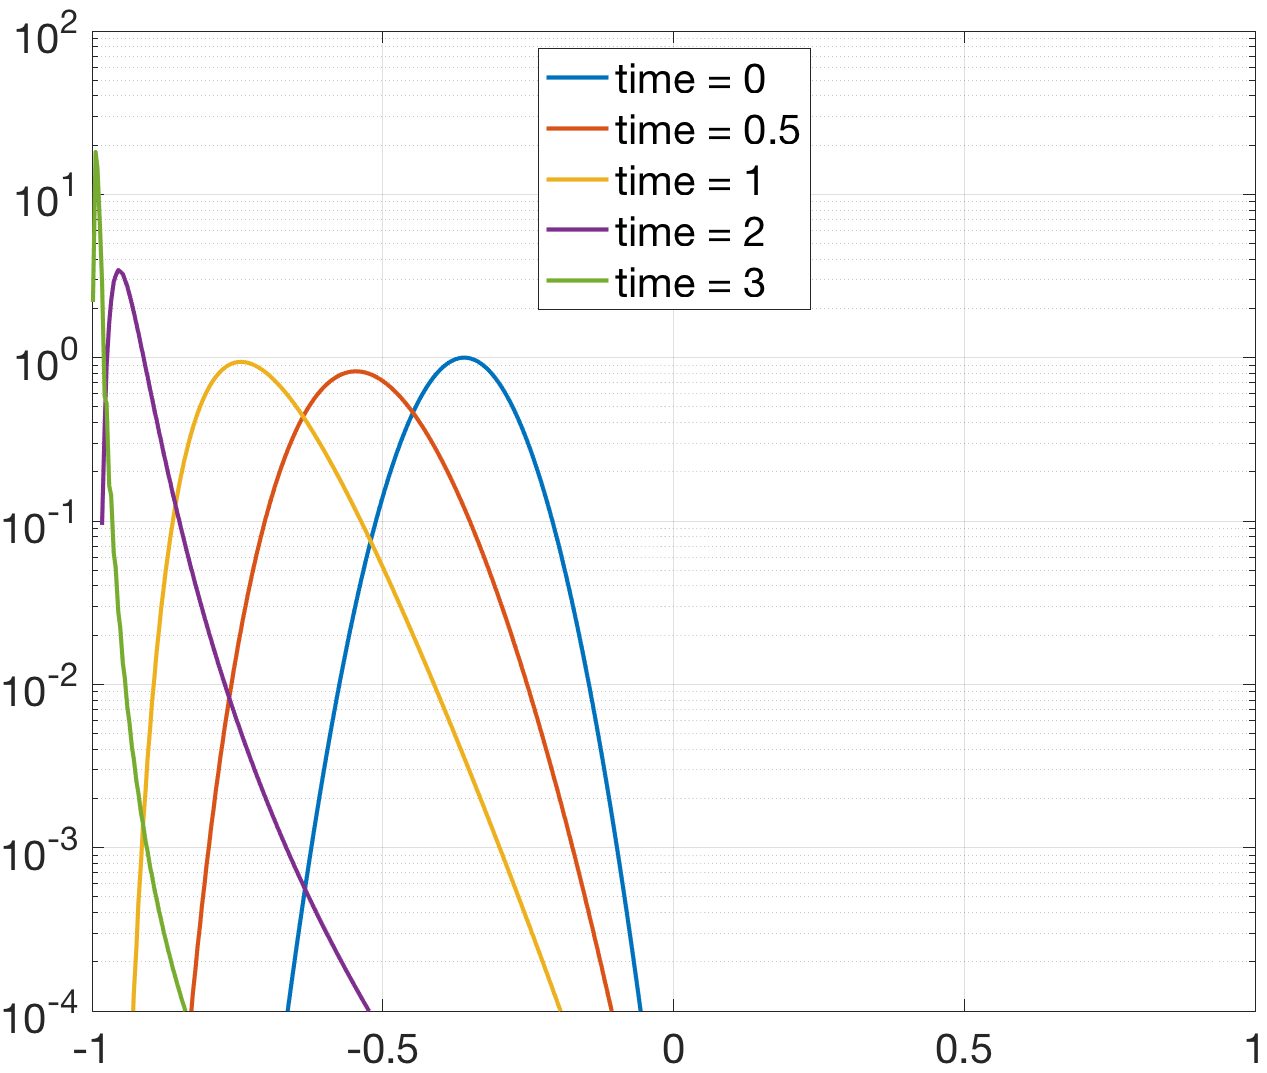
\includegraphics[width=.3\textwidth]{./NumFig/Test4-3-2-L8D2-log}
&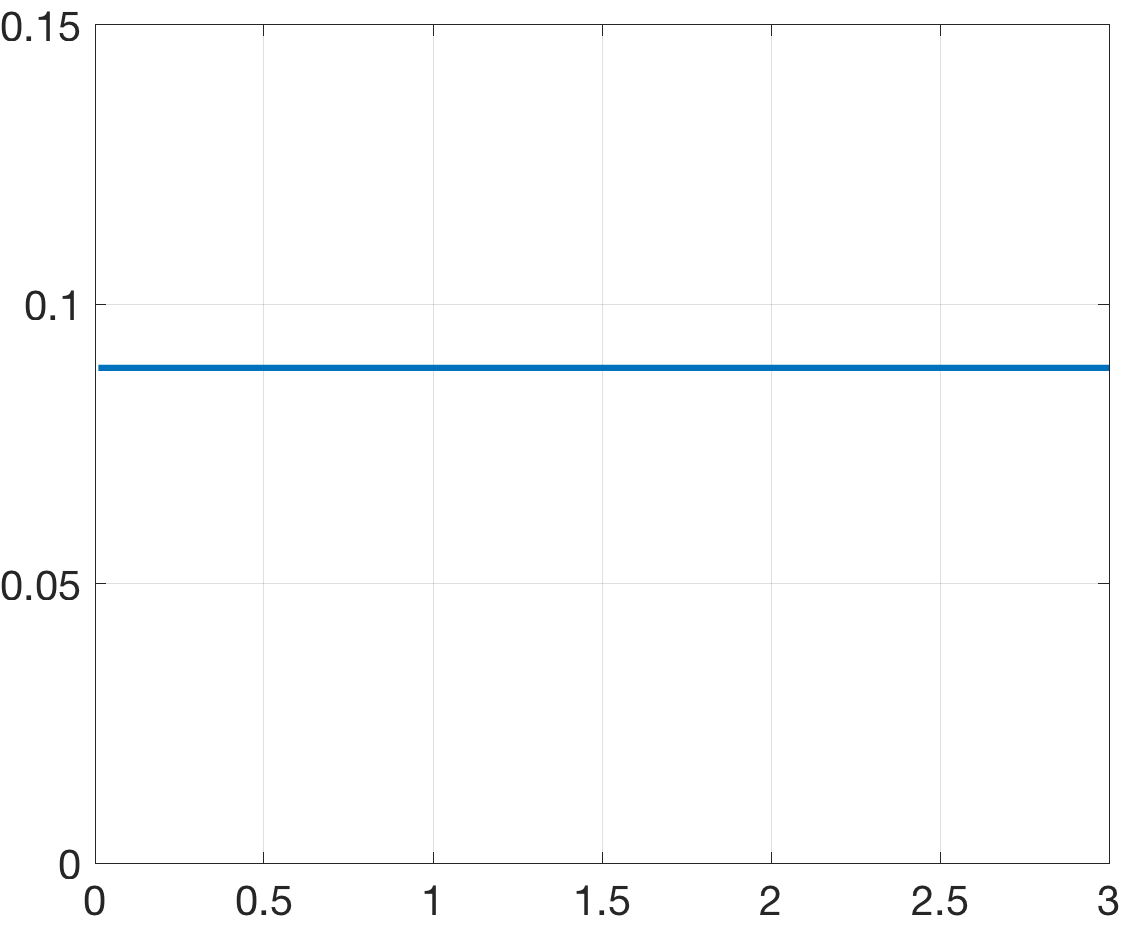
\includegraphics[width=.3\textwidth]{./NumFig/Test4-3-k1-2-Con_v2}
\\
(a) & (b) &(c)
\end{tabular}
\caption{Test~\ref{Subsec:Pitch-3} (case 3): Plots of numerical solutions at time $=0,0.5,1,2,3$ on mesh with $N$ = 8, $k=1$: (a) Plot of numerical solutions; (b) semilog plot of numerical solutions; (c) plot of total mass.}\label{Fig:Pitch-3-3}
\end{figure}

\begin{figure}[H]
\centering
\begin{tabular}{ccc}
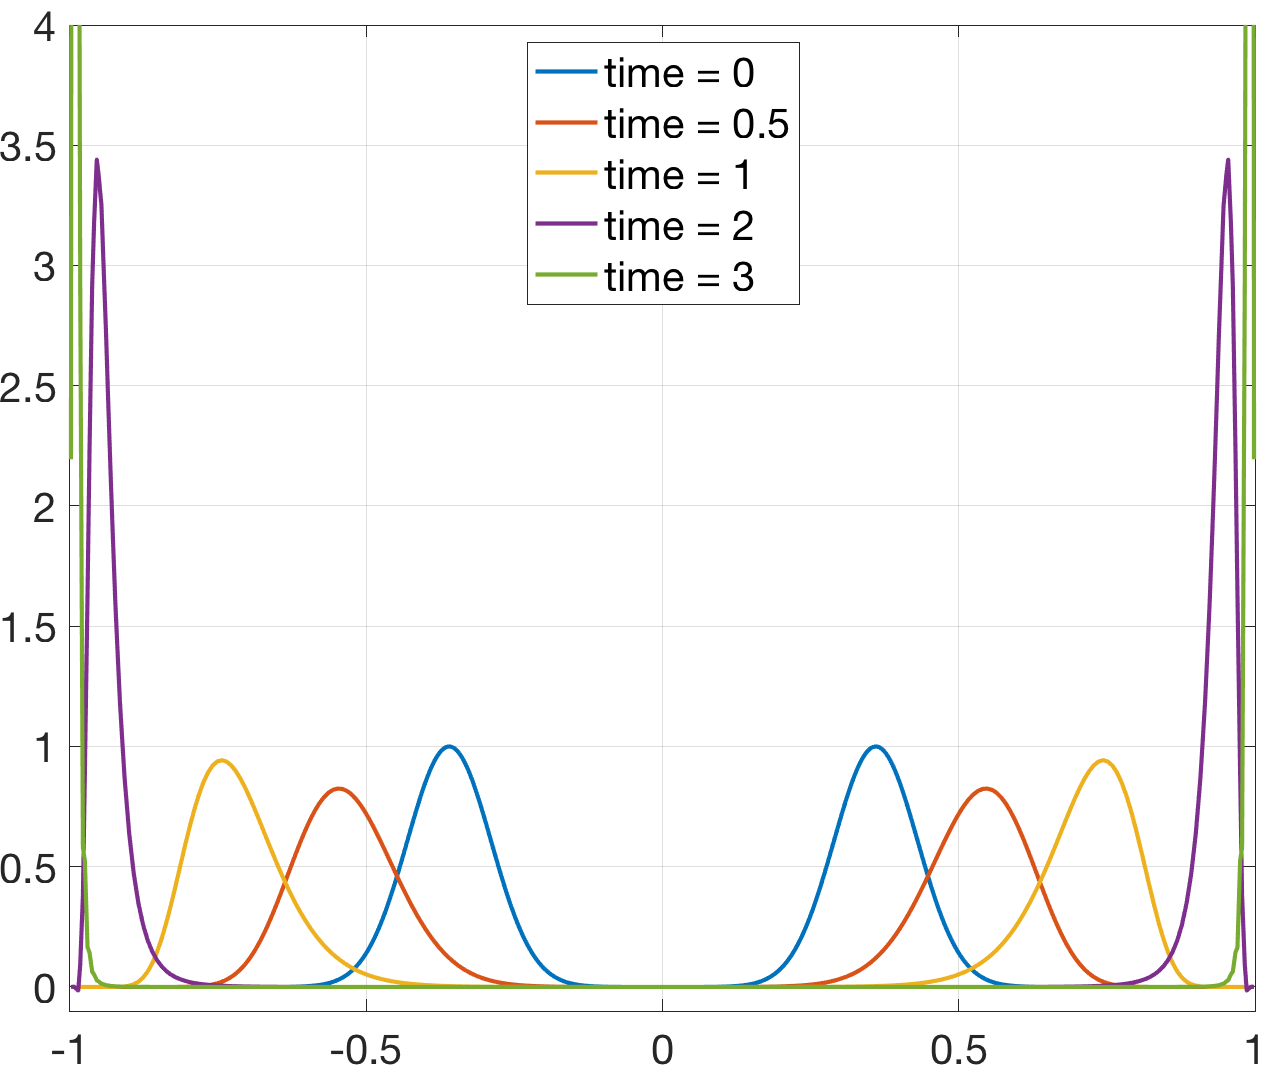
\includegraphics[width=.3\textwidth]{./NumFig/Test4-3-4-L8D2}
&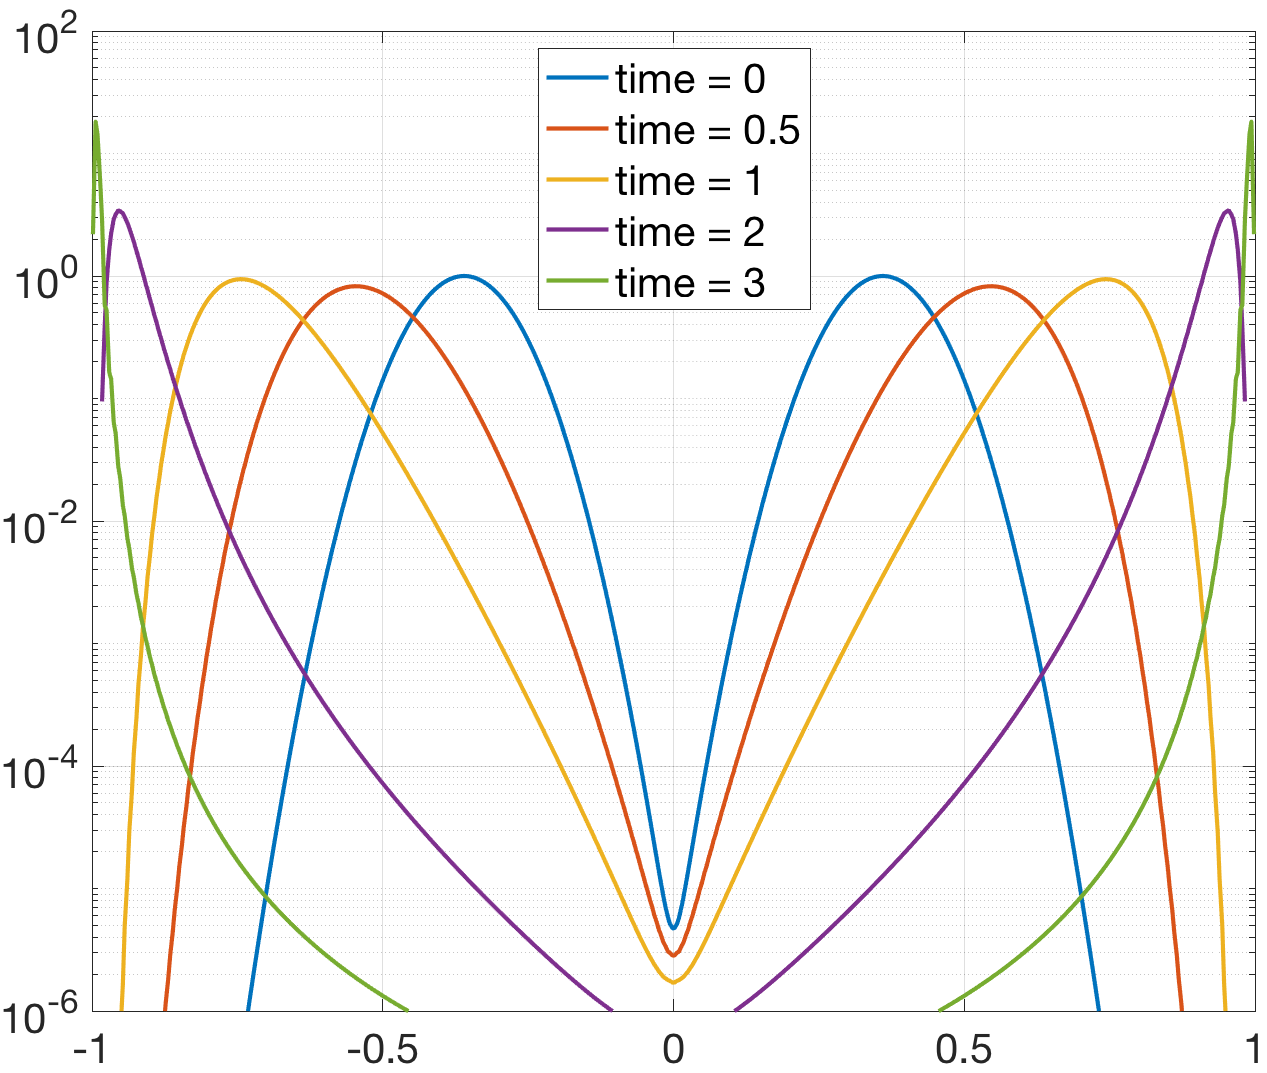
\includegraphics[width=.3\textwidth]{./NumFig/Test4-3-4-L8D2-log}
&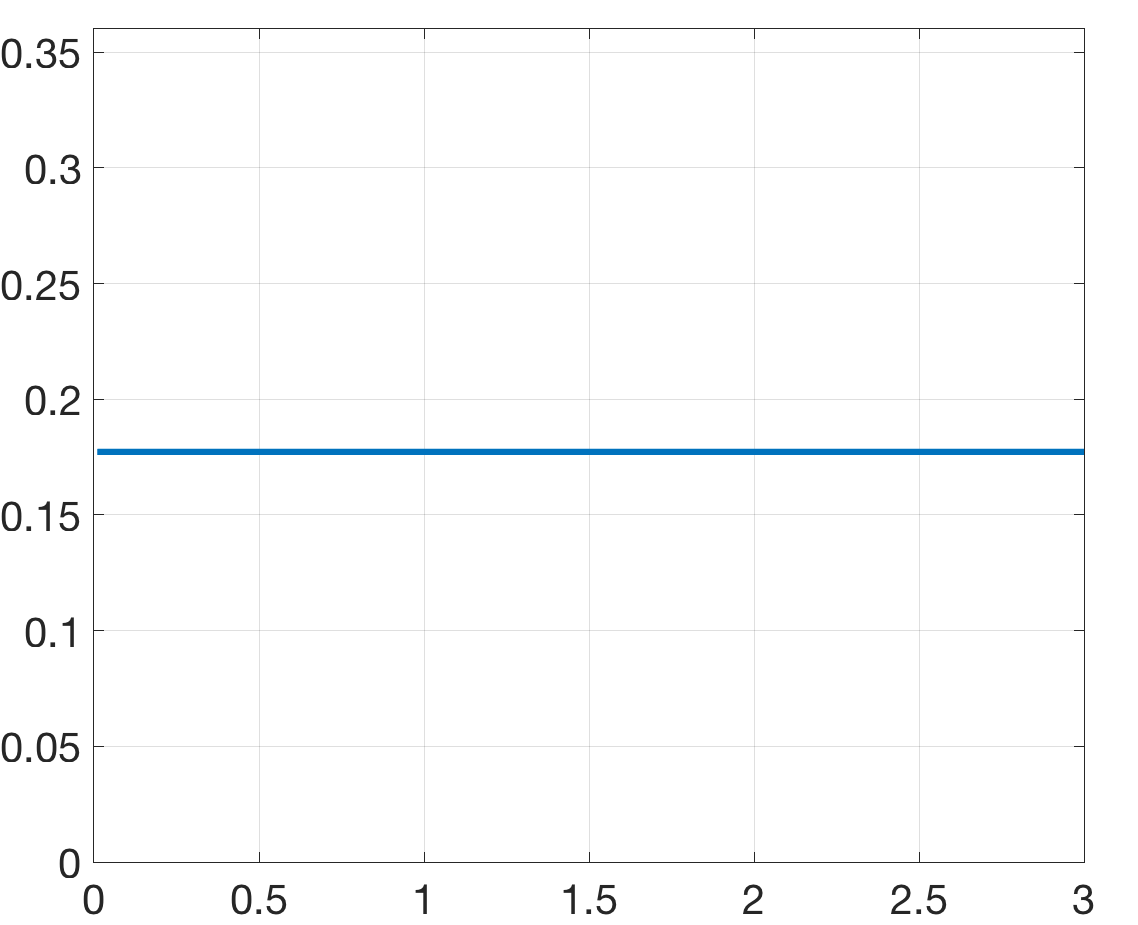
\includegraphics[width=.3\textwidth]{./NumFig/Test4-3-k1-4-Con_v2}
\\
(a) & (b) &(c)
\end{tabular}
\caption{Test~\ref{Subsec:Pitch-3} (case 4): Plots of numerical solutions at time $=0,0.5,1,2,3$ on mesh with $N$ = 8, $k=1$: (a) Plot of numerical solutions; (b) semilog plot of numerical solutions; (c) plot of total mass.}\label{Fig:Pitch-3-4}
\end{figure}


\subsection{Pitch Angle - Combined electric field and collision term testing (R=0)}
\label{Subsec:Pitch-4}
The evolution of the pitch angle dependence of $f$ in the presence of electric field acceleration and collisions is governed by the equation
%
\bq
\label{pitch_E_coll_eq}
\frac{\partial f}{\partial t}= 
- E \frac{\partial}{\partial\xi} \left[ \left(1-\xi^2\right) f \right] + C \frac{\partial}{\partial\xi} \left[ \left(1-\xi^2\right) \frac{\partial f}{\partial \xi} \right]\, ,
\eq
%
with initial and boundary conditions given in Eq.~(\ref{ic_bc}). In the finite element simulation, we shall choose alternating flux for the collision operator and upwind flux for the electric field acceleration.

\noindent{\bf Test~\ref{Subsec:Pitch-4}} In this test, we shall use the following steady-state solution as the reference solution and check the proposed numerical scheme:
\bq
\label{pitch_E_coll_sol}
f(\xi)=\frac{A}{2 \sinh A} e^{A \xi}\, , \qquad A=E/C \, ,
\eq
where the pre-factor in the exponential is a normalization factor. 

For $C = 1$, the numerical solution for different values of $A$ are plotted in Figure~\ref{fig:pitch_E_coll}.

\begin{figure}[H]
\centering
\begin{tabular}{cc}
  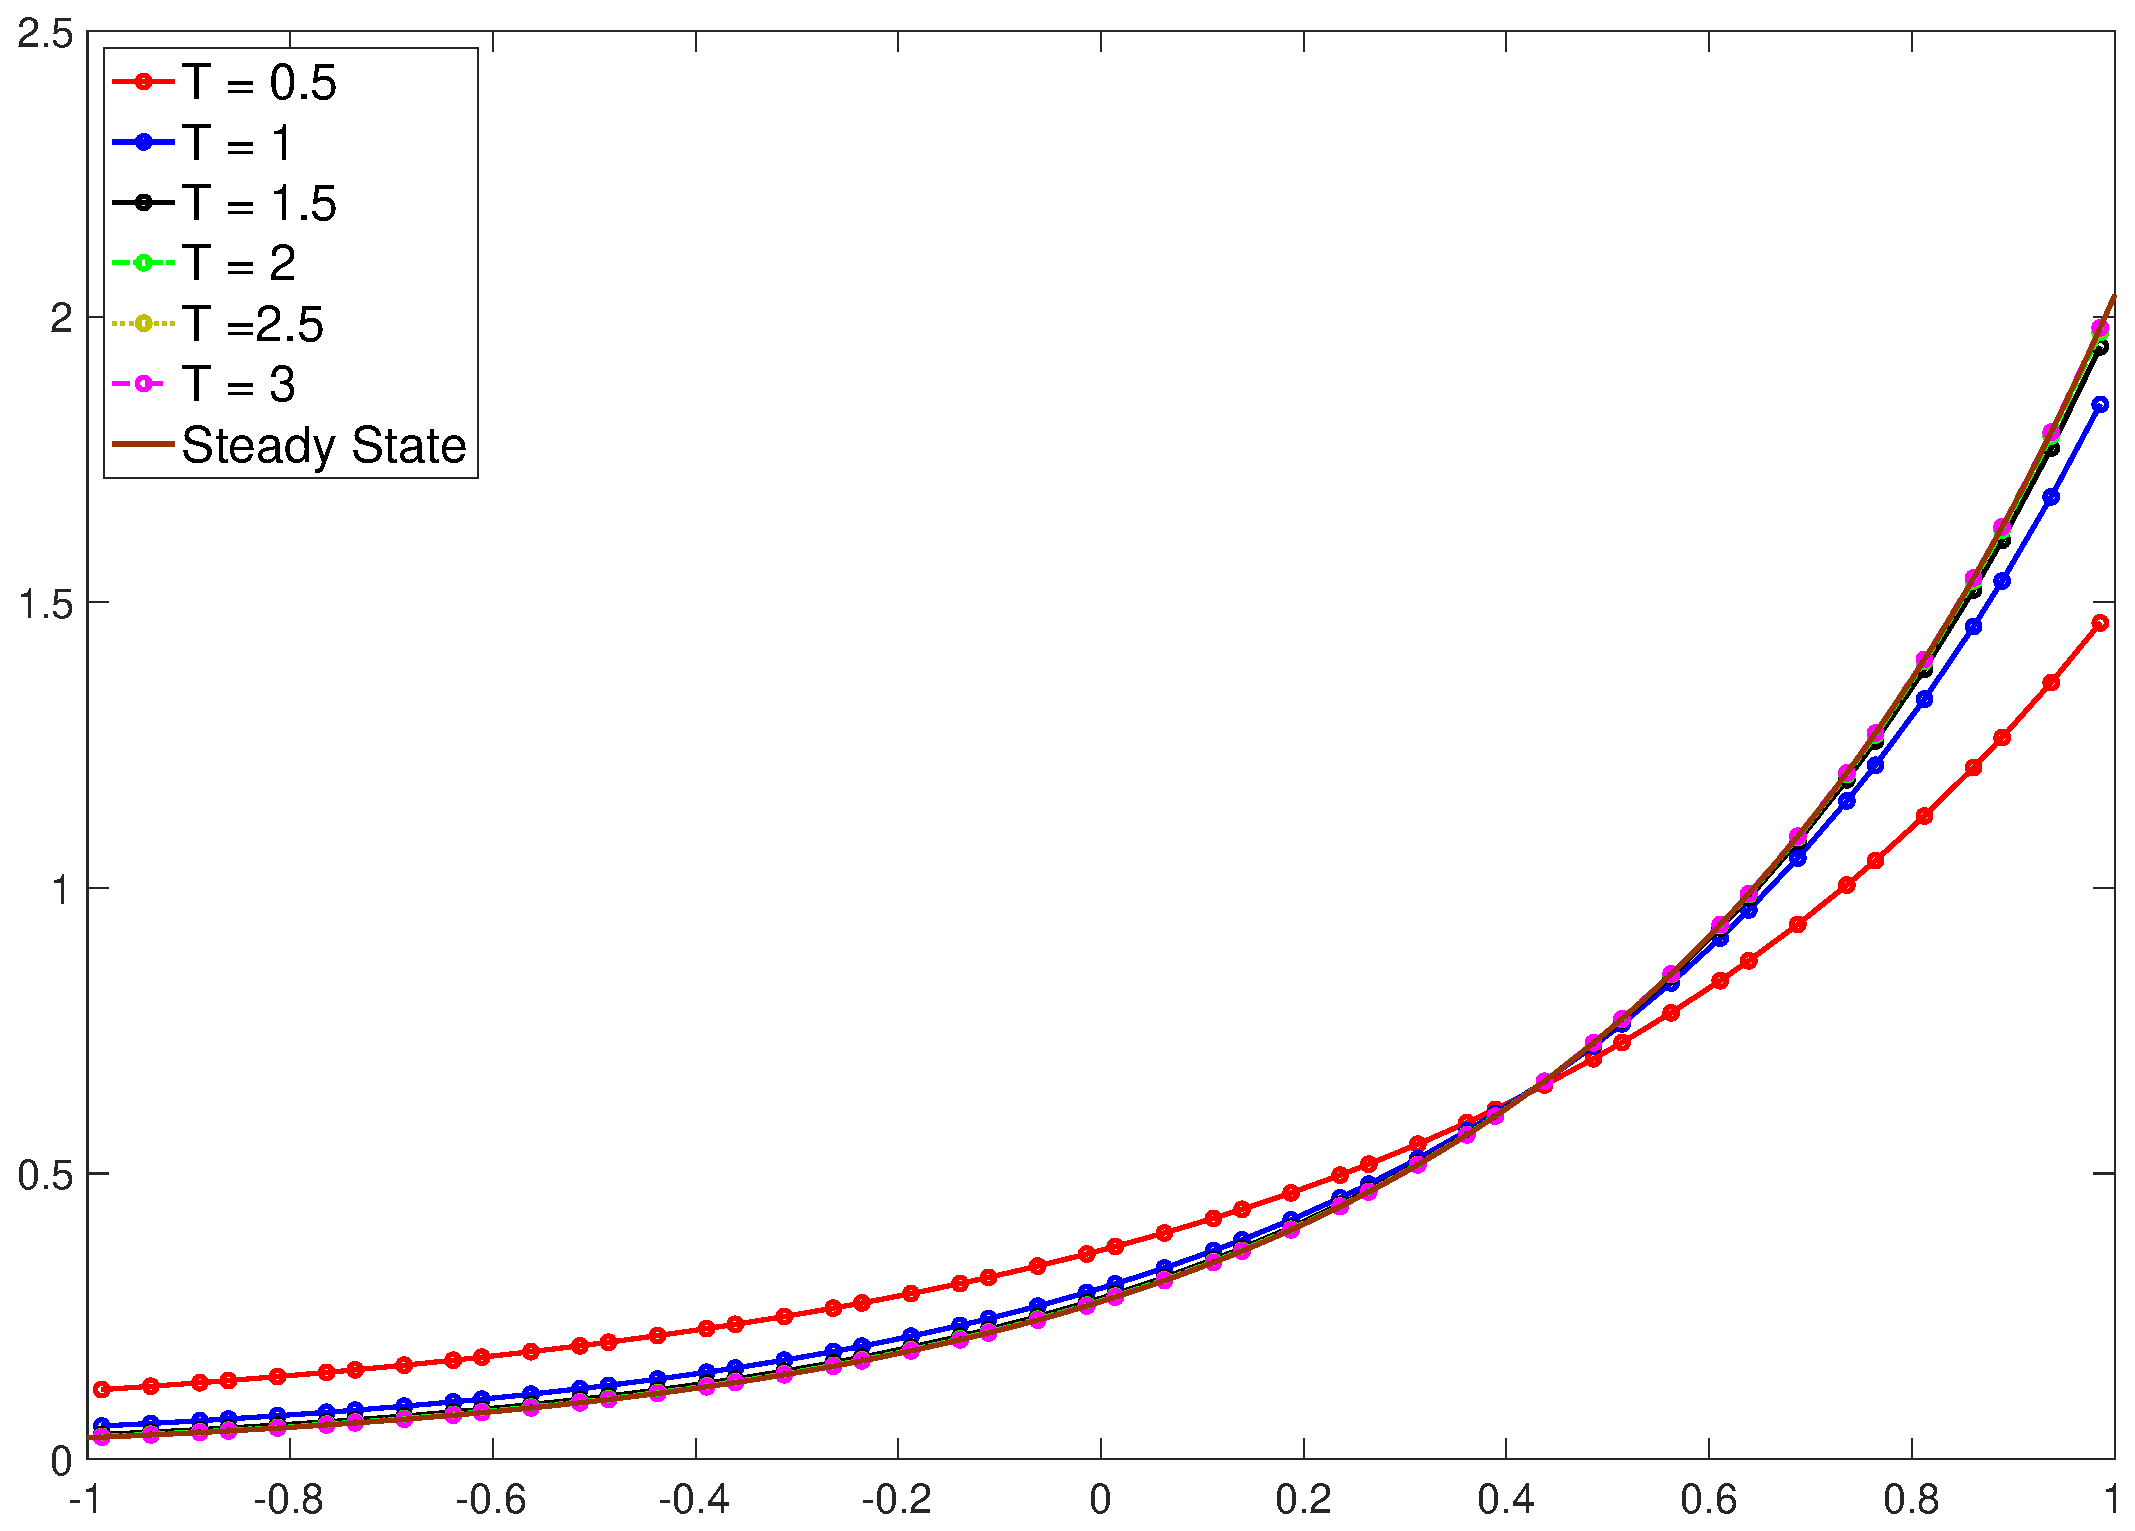
\includegraphics[width=.45\textwidth]{./NumFig/condiff-uf-E2_v2}
  &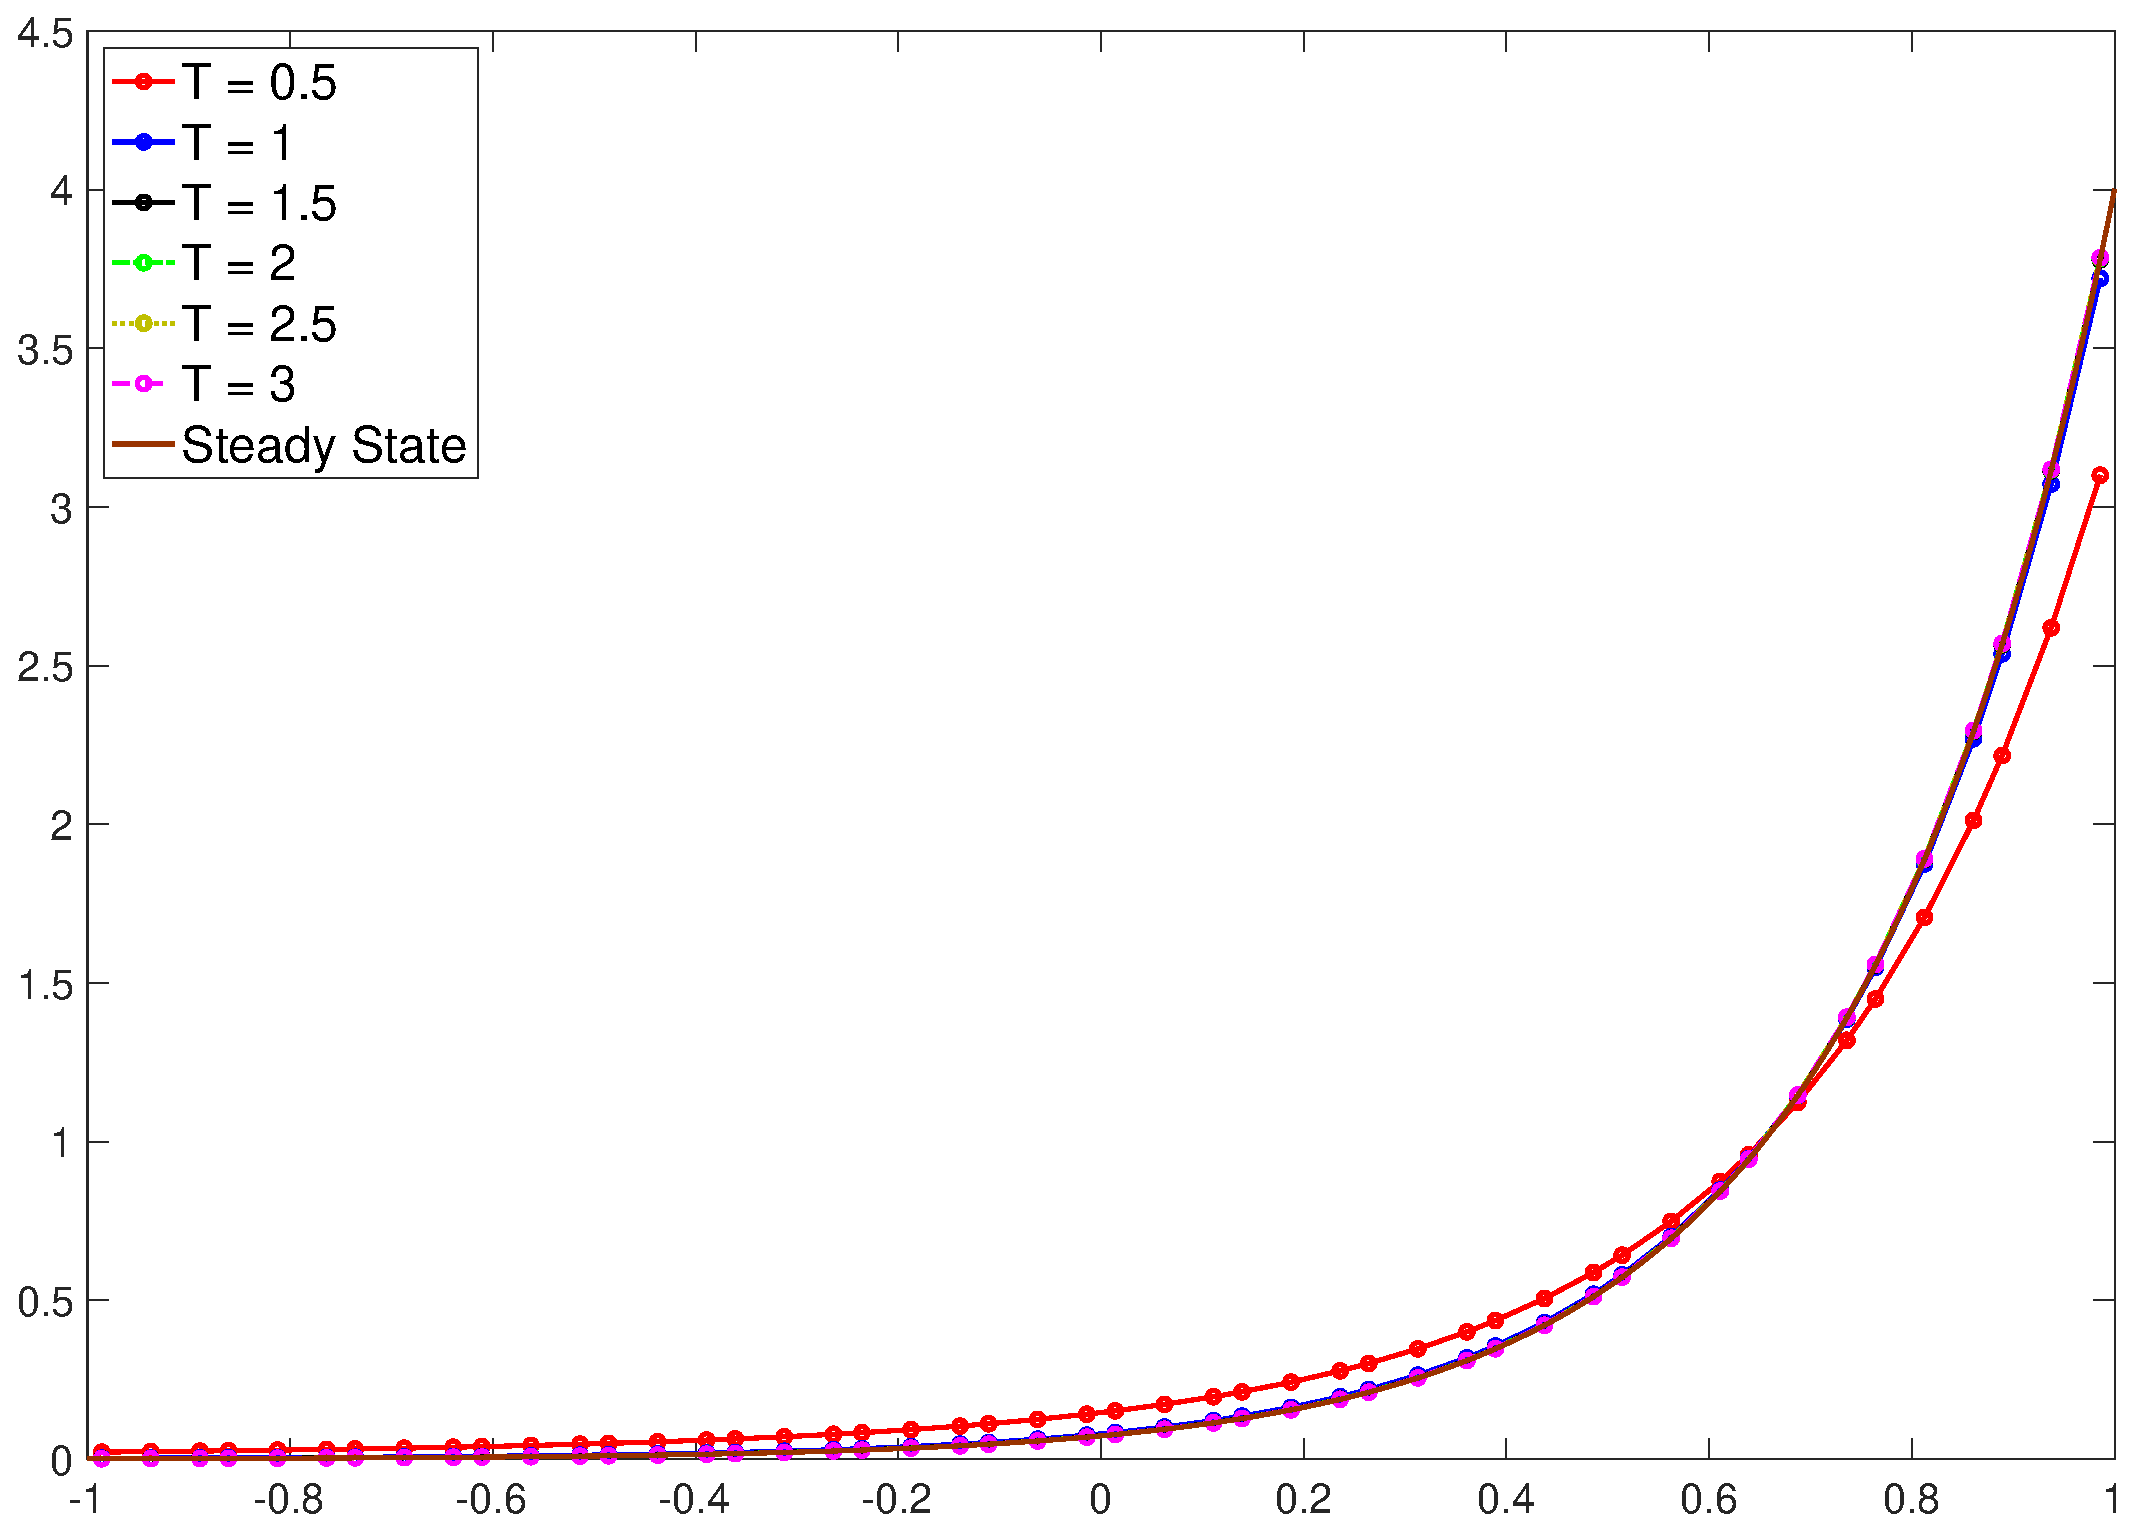
\includegraphics[width=.45\textwidth]{./NumFig/condiff-uf-E4_v2}\\
  (a) & (b)
  \end{tabular}
\caption{Test~\ref{Subsec:Pitch-4}: Plot for numerical solution solutions for $N$ = 4, $k = 4$ of upwind flux at time = 0.5, 1, 1.5, 2, 2.5, 3: (a) of $E=2$; (b) of $E = 4$.}\label{fig:pitch_E_coll}
\end{figure}


\subsection{Complete Pitch Angle Dynamics}
\label{Subsec:Pitch-5}
The evolution of the pitch angle dependence of $f$ in the presence of electric field acceleration, collisions, and radiation damping is governed by the equation (\ref{pitch_full_eq})
where $E$, $C$, and $R$ are constants, and the initial and boundary conditions are given in Eq.~(\ref{ic_bc}). In the numerical implementation, we shall take the collision operator with alternating flux and employ the other operators with upwind flux.

\vskip.1in
\noindent{\bf Test~\ref{Subsec:Pitch-5}}
In this test, we shall use the following steady-state solution as the reference solution for testing:
\bq
\label{pitch_full_sol}
f(\xi)= Q \exp \left[ {A\, \xi + (B/2) \, \xi^2}\right] \, , \qquad A=\frac{E}{C} \, , \qquad B=\frac{R}{C} \, ,
\eq
where $Q$ is a normalization constant. Figure~\ref{Fig:pitch_full} (a) and (b) show plots of this solution and numerical solutions for different values of $E/C$ and $R/C$.
%
\begin{figure}[H]
\centering
\begin{tabular}{cc}
 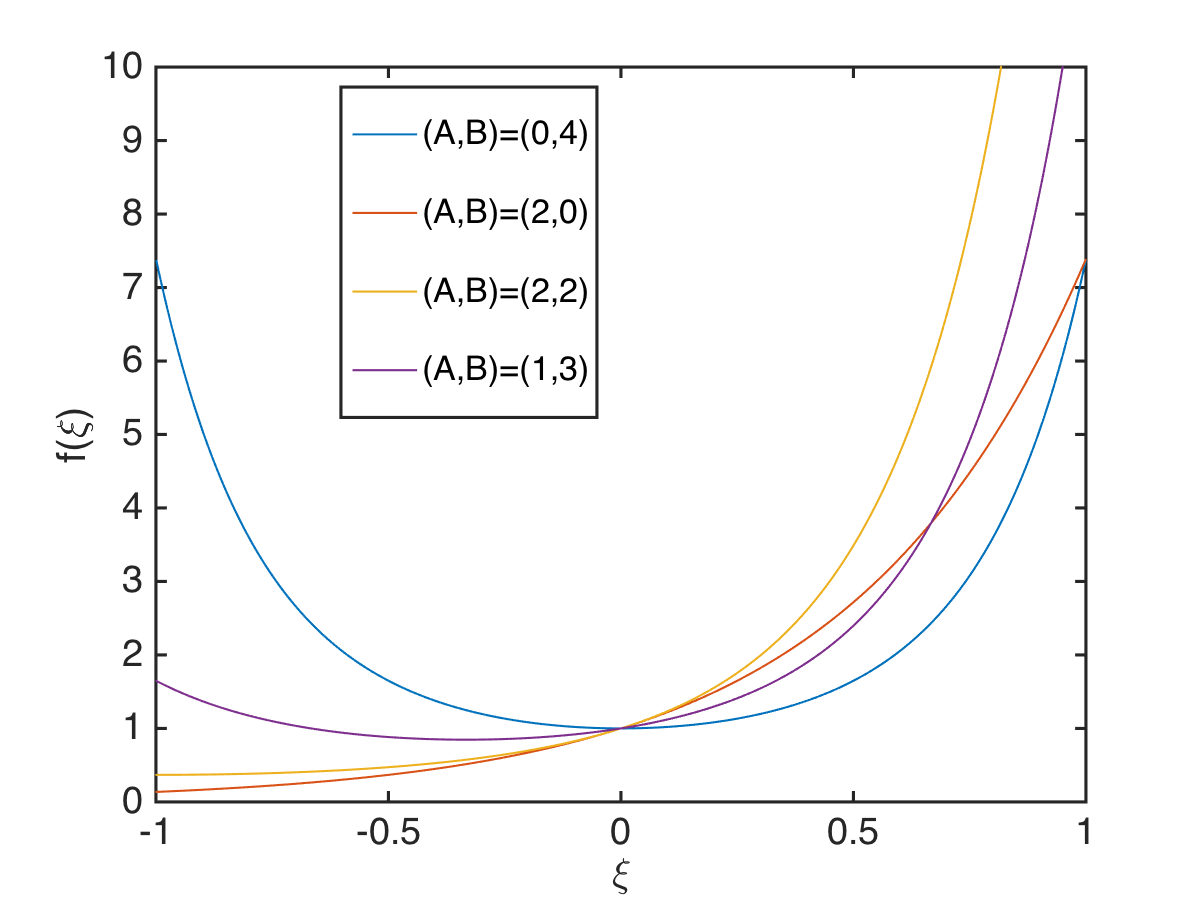
\includegraphics[width=.45\textwidth,height=.4\textwidth]{FIGURES/fig_pitch_full}
  &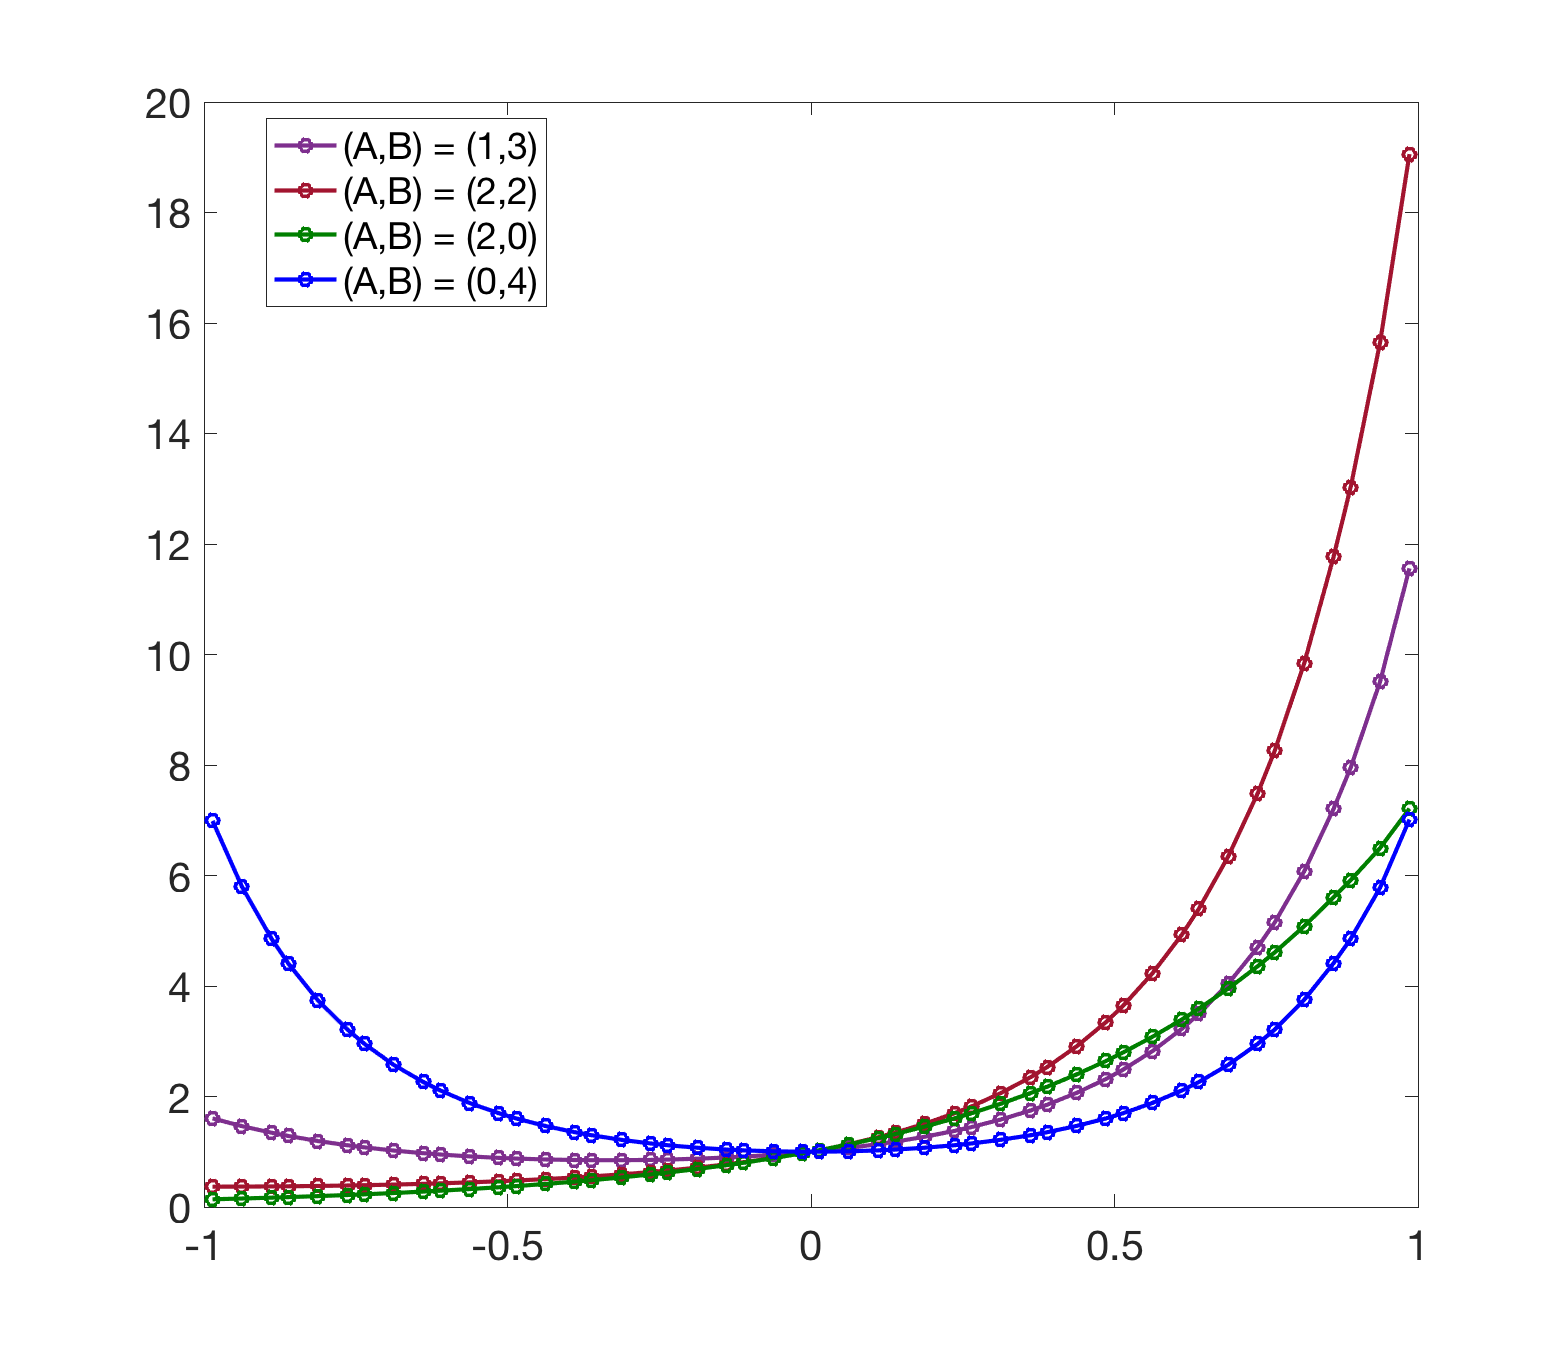
\includegraphics[width=.45\textwidth,height=.4\textwidth]{./NumFig/test_full}\\
  (a) & (b)
  \end{tabular}
\caption{Test~\ref{Subsec:Pitch-5}: (a) Analytical steady-state solution of Eq.~(\ref{pitch_full_eq}) according to Eq.~(\ref{pitch_full_sol}) different values of  $A=E/C$, and $B=R/C$; (b) Corresponding numerical solutions.}\label{Fig:pitch_full}
\end{figure}


\subsection{Numerical Scheme for 1D Momentum Dynamics} 
\label{sec:Mom}
The full, 1-D momentum dynamics are governed by the equation (\ref{pitch_full_eq}) with boundary conditions
\bq
\left. \frac{\partial f (p,t)}{\partial p}\right|_{p=0}=0 \, , \qquad f(p=p_{max},t)=0 \, ,
\eq
where $p_{max} \gg m v_{th}$. 
The steady-state solution of this equation is
\bq
f(p)=Q \exp \left[-\frac{1}{m T} \int \frac{p}{\sqrt{1+(p/mc)^2}} dp \right]
\exp \left[\int \left( \frac{E}{C_A} -\frac{R}{C_A} p  \sqrt{1+(p/mc)^2} \right) dp \right] \, ,
\eq
where $Q$ is a normalization constant, $m$ is the rest mass of the electron and $T$ the plasma temperature. 
In the non-relativistic limit, $p/mc\rightarrow 0$ and in the absence of electric field and radiation damping, $E=R=0$, the steady-state reduces to the expected Maxwellian distribution 
\bq
\label{eq_maxwell}
f(p)=Q \exp \left[-\frac{p^2}{2m T} \right]= Q \exp \left[-\left(\frac{v}{v_{th}}\right)^2 \right] \, ,
\eq
where $v_{th}=\sqrt{2 T/m}$ is the plasma thermal temperature. 

Next, we shall consider the momentum dynamics, which is governed by the following equation: 
%
\begin{eqnarray}
\label{momentumdynamiceq}
    \frac{\partial f}{\partial t} = \frac{1}{p^2}\frac{\partial}{\partial p}p^2\left[C_A\frac{\partial f}{\partial p}+C_Ff\right]-\frac{E}{p^2}\frac{\partial}{\partial p}\left[p^2f\right]+R\frac{1}{p^2}\frac{\partial}{\partial p}\left[p^3\gamma f\right].\label{pitch_full_eq}
\end{eqnarray}
Denoting $g = \dfrac{\partial f}{\partial p}$, equation (\ref{momentumdynamiceq}) can also be expressed as a system of equations:
\begin{eqnarray}
g &=& \frac{\partial f}{\partial p},\label{numericalmomentumeq1}\\%[10pt]
p^2\dfrac{\partial f}{\partial t} &=& \frac{\partial}{\partial p} \big(p^2C_A g+p^2C_Ff\big) -{E}\frac{\partial}{\partial p}(p^2f)+ R\frac{\partial}{\partial p} \big(p^3\gamma f\big).\label{numericalmomentumeq2}
\end{eqnarray}
The finite element space can be chosen as $V_k^N$ for the momentum variable $p$. Again, multiplying both equations by test functions $\Theta$ and $\Xi$, and integrating over cell $I_j^N$ ($j = 0,\cdots,2^N-1$), using integration by parts yields, 
\begin{eqnarray}
\label{numericalschememomentum1}
(g_h,\Theta) &=& \mathcal{G}_p(f_h,\Theta),\ \forall\Theta\in V_h\\
%%%
\label{numericalschememomentum2}
(p^2\frac{\partial f_h}{\partial t},\Xi)
&=&\mathcal{C}_{A,p}(g_h,\Xi) + \mathcal{C}_{F,p}(f_h,\Xi)+\mathcal{E}_{p}(f_h,\Xi)+\mathcal{R}_{p}(f_h,\Xi),\ \forall\Xi\in V_h.
\end{eqnarray}
Here the bilinear forms are defined as:
\begin{eqnarray}
\mathcal{G}_p(w,v) &=& -\sum_{K_p\in \mathcal{T}_{h,p}}\int_{K_p}w\frac{\partial v}{\partial p}dp+\sum_{j=0}^{2^N}\left[\lavg\widehat{w}\ravg\ljump v\rjump\right]_{p_j},\\
%%%
\mathcal{C}_{A,p}(w,v) &=& -\sum_{K_p\in \mathcal{T}_{h,p}}\int_{K_p}(C_Ap^2w)\dfrac{\partial\Theta}{\partial p}dp+\sum_{j=0}^{2^N}\left[\lavg C_Ap^2\hat{w}\ravg\ljump v\rjump\right]_{p_j},\\
%%%
\mathcal{C}_{F,p}(w,v) &=& -\sum_{K_p\in \mathcal{T}_{h,p}}\int_{K_p}(C_Fp^2w)\dfrac{\partial\Theta}{\partial p}dp+\sum_{j=0}^{2^N}\left[\lavg C_Fp^2\hat{w}\ravg\ljump v\rjump\right]_{p_j},\\
%%%
\mathcal{E}_p(w,v)&=&\sum_{K_p\in \mathcal{T}_{h,p}}\int_{K_p}(Ep^2w)\frac{\partial v}{\partial p}dp-\sum_{j=0}^{2^N}\left[\lavg Ep^2 \hat{w}\ravg\ljump v\rjump\right]_{p_j},\\
%%%
\mathcal{R}_{p}(w,v)&=& -\sum_{K_p\in \mathcal{T}_{h,p}}\int_{K_p}(Rp^3\gamma w)\frac{\partial v}{\partial p}dp+\sum_{j=0}^{2^N}\left[\lavg Rp^3\gamma\hat{w}\ravg\ljump v\rjump\right]_{p_j}.
\end{eqnarray}
Here the term $\lavg\hat{\cdot}\ravg$ denote the numerical flux on the edge $e$. Similar as the pitch angle approximation, the three choices for numerical flux can be utilized here. 
%
- Notes on how numerical quadrature is performed \todo{**LIN**{\color{blue}Are we expecting the description of Gaussian quadrature here?}}  


\subsubsection{Momentum - Collision term testing (E=R=0)}
\label{Subsec:mom-collisions}
As a starting point, we should check that the numerical solution converges to the Maxwellian in the non-relativistic limit with $E=R=0$. That is, reduce the problem to the solution of
\bq
\frac{\partial f}{\partial t}=\frac{1}{p^2} \frac{\partial}{\partial p} p^2 \left[ C_A \frac{\partial f}{\partial p} + C_F f\right] \, .
\eq

In this test, we will use the non-dimensional variable $p=v/v_{th}$, rescale the time $t$, and write the Fokker-Planck equation as
\bq
\frac{\partial f}{\partial t}=\frac{1}{p^2} \frac{\partial}{\partial p} p^2 \left[ \frac{\psi(p)}{p}\frac{\partial f}{\partial p} + 2 \psi(p) f\right] \, ,
\eq
where $\psi(p)$ is defined as:
\begin{eqnarray}
\phi(p)=\mathrm{erf}(p)=\frac{2}{\sqrt{\pi}}\int_0^p e^{-s^2}ds,\ \psi(x)=\frac{1}{2p^2}\bigg(\phi(p)-p\frac{d\phi}{dp}\bigg).
\end{eqnarray}
The boundary conditions are:
\bq
\left. \frac{\partial f (p,t)}{\partial p}\right|_{p=0}=0 \, , \qquad f(p=p_{\max},t)=0 \, ,
\eq
where $p_{\max} \gg 1$. For these variables, according to Eq~(\ref{eq_maxwell}) the steady-state is simply $\frac{4}{\sqrt{\pi}}e^{-p^2}$.%$f(x)=Q e^{-x^2}$.  
The numerical experiment is carried out by assuming $p_{\max}=10$.

\noindent{\bf Test~\ref{Subsec:mom-collisions}a} (collision-test-1). The first test is to choose initial condition as $\frac{4}{\sqrt{\pi}a^3}e^{-p^2/a^2}$ and set $a=2$.

The numerical solutions are plotted at different time in Figure~\ref{Fig:Mom-1} and the plot for total mass is present in the right panel. As one can observe the mass preserving during all the time.

Besides, in this test, we run the numerical simulation until the difference of $f^{n-1}$ and $f^n$ is less than $10^{-10}$ and this requires the end time as $340$. The comparison of numerical solution at $t = 340$ with steady-state is reported in Table~\ref{Tab:Mom-1}. It can be observed that the rate for convergence is $\mathcal{O}(h^{k+1})$. In the cubic element's simulation, $10^{-10}$ is not a good enough approximation of the steady-state solution, and when $N$ is bigger than 8, the optimal convergence rate cannot be preserved.
%
\begin{figure}[H]
\centering
\begin{tabular}{cc}
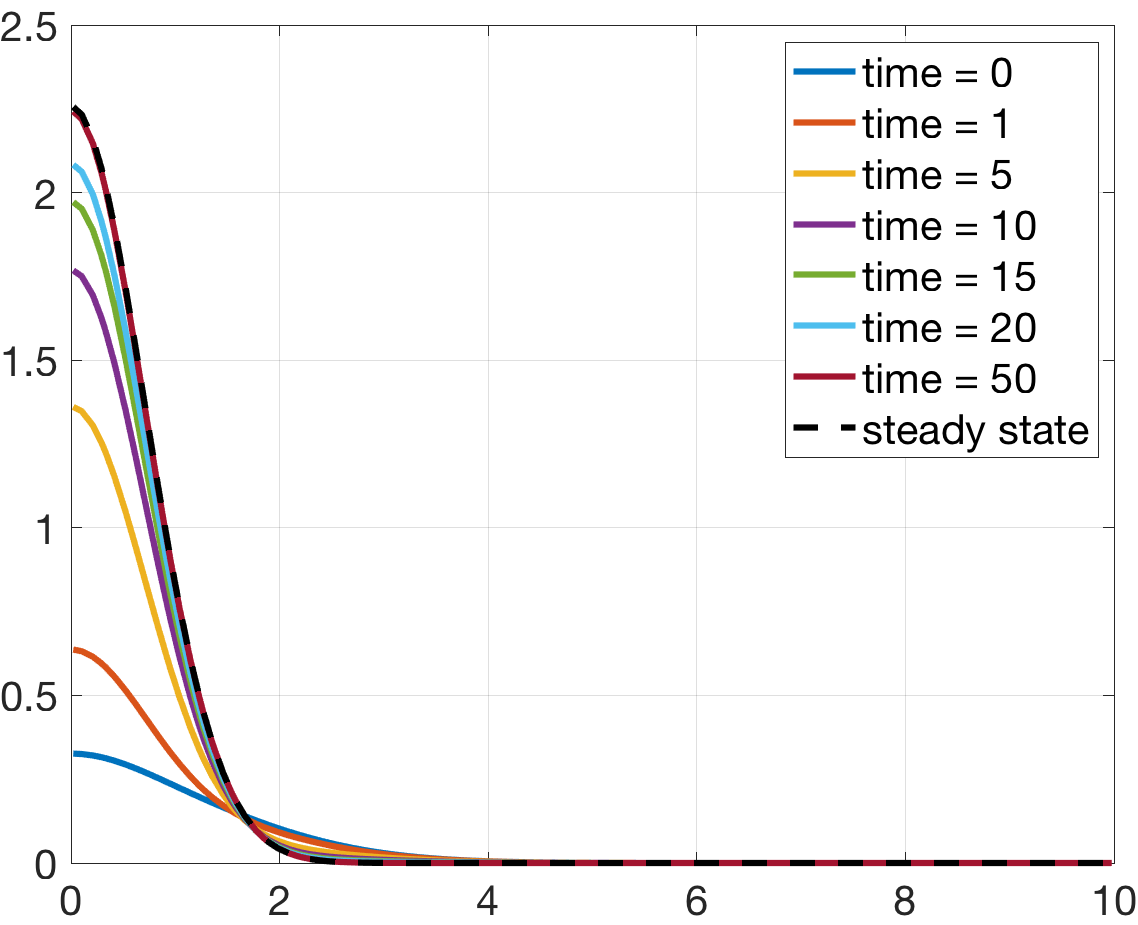
\includegraphics[width=.45\textwidth,height = .3\textwidth]{./NumFig/Ini-Mom-1}
&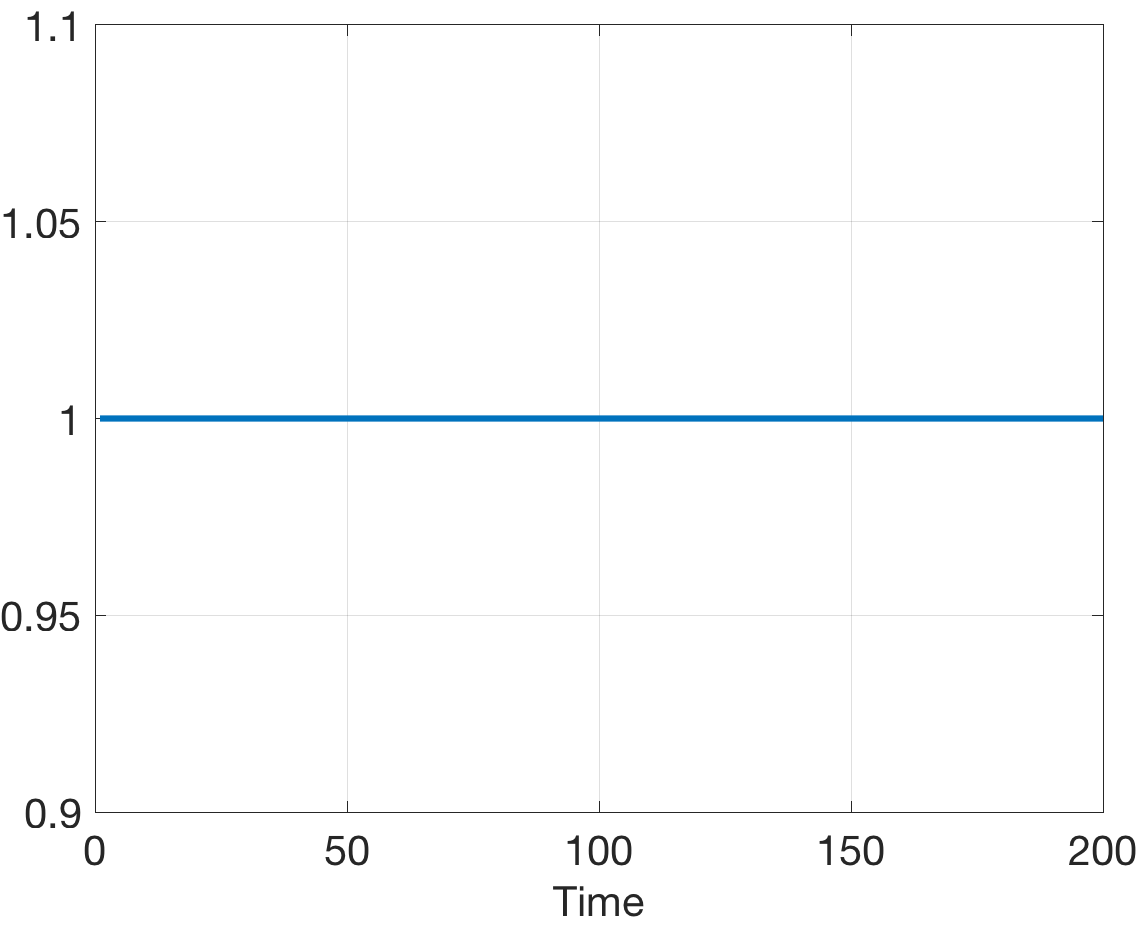
\includegraphics[width=.45\textwidth,height = .3\textwidth]{./NumFig/Ini-Mom-1-Conv.png}\\
(a) & (b)
\end{tabular}
\caption{Test~\ref{Subsec:mom-collisions}a: Plot of numerical solution for alternating flux: (a) plot of numerical solution at different time; (b) the plot for total mass.}\label{Fig:Mom-1}
\end{figure}

{\small
\begin{table}[H]
\caption{Test~\ref{Subsec:mom-collisions}a: Error profiles and convergence test for upwind flux.}\label{Tab:Mom-1}
\centering
\begin{tabular}{c|cc|cc}	\hline\hline
$N$ & $\|f-f_h\|_{\infty}$ & Rate & $\|f-f_h\|$ & Rate \\ \hline		
&\multicolumn{4}{c}{$k=1$}\\ \hline
4	&5.2864E-02	&		&5.2892E-02	&\\
5	&2.5388E-02	&1.06	&1.4358E-02	&1.88\\
6	&6.5526E-03	&1.95	&3.6769E-03	&1.97\\
7	&1.5249E-03	&2.10	&9.1786E-04	&2.00\\
8	&3.5857E-04	&2.09	&2.2854E-04	&2.01\\
9	&8.6355E-05	&2.05	&5.6976E-05	&2.00\\
10	&2.1152E-05	&2.03	&1.4222E-05	&2.00\\ \hline
&\multicolumn{4}{c}{$k=2$}\\ \hline		
4	&9.1049E-03	&		&7.4916E-03	&\\
5	&1.1269E-03	&3.01	&8.7676E-04	&3.10\\
6	&1.4136E-04	&2.99	&1.0205E-04	&3.10\\
7	&1.7600E-05	&3.01	&1.2460E-05	&3.03\\
8	&2.1939E-06	&3.00	&1.5457E-06	&3.01\\
9	&2.7141E-07	&3.01	&1.9264E-07	&3.00\\
10	&3.1662E-08	&3.10	&2.4195E-08	&2.99\\ \hline
&\multicolumn{4}{c}{$k=3$}\\ \hline				
4	&6.7085E-04	&		&5.3862E-04	&\\
5	&4.7544E-05	&3.82	&3.6259E-05	&3.89\\
6	&3.6905E-06	&3.69	&2.4362E-06	&3.90\\
7	&2.4618E-07	&3.91	&1.5398E-07	&3.98\\
8	&1.8430E-08	&3.74	&9.9121E-09	&3.96\\
9	&4.0258E-09	&2.19	&2.4803E-09	&2.00\\
10	&4.2010E-09	&-       	&3.2612E-09	&- \\ \hline
\hline
\end{tabular}
\end{table}
}

\noindent{\bf Test~\ref{Subsec:mom-collisions}b}. The second test is to choose the initial condition as
$$
f = \begin{cases}
\frac{3}{5^3},\ p\in[0,5],\\
0,\text{ \ \ else}.
\end{cases}
$$

{\small
\begin{table}[H]
\caption{Test~\ref{Subsec:mom-collisions}b: Error profiles and convergence test for upwind flux.}\label{Tab:Mom-2}
\centering
\begin{tabular}{c|cc|cc}	\hline\hline
$N$ & $\|f-f_h\|_{\infty}$ & Rate & $\|f-f_h\|$ & Rate \\ \hline		
&\multicolumn{4}{c}{$k=1$}\\ \hline
4	&5.2865E-02	&		&5.2892E-02	&\\
5	&2.5388E-02	&1.06	&1.4358E-02	&1.88\\
6	&6.5526E-03	&1.95	&3.6769E-03	&1.97\\
7	&1.5249E-03	&2.10	&9.1786E-04	&2.00\\
8	&3.5858E-04	&2.09	&2.2854E-04	&2.01\\
9	&8.6356E-05	&2.05	&5.6976E-05	&2.00\\
10	&2.1154E-05	&2.03	&1.4222E-05	&2.00 \\ \hline		
&\multicolumn{4}{c}{$k=2$}\\ \hline
4	&9.1049E-03	&		&7.4916E-03	&\\
5	&1.1269E-03	&3.01	&8.7676E-04	&3.10\\
6	&1.4137E-04	&2.99	&1.0205E-04	&3.10\\
7	&1.7602E-05	&3.01	&1.2460E-05	&3.03\\
8	&2.1953E-06	&3.00	&1.5456E-06	&3.01\\
9	&2.7289E-07	&3.01	&1.9263E-07	&3.00\\
10	&3.3138E-08	&3.04	&2.4072E-08	&3.00 \\ \hline		
&\multicolumn{4}{c}{$k=3$}\\ \hline
4	&6.7084E-04	&		&5.3862E-04	&\\
5	&4.7546E-05	&3.82	&3.6259E-05	&3.89\\
6	&3.6887E-06	&3.69	&2.4361E-06	&3.90\\
7	&2.4439E-07	&3.92	&1.5396E-07	&3.98\\
8	&1.6609E-08	&3.88	&9.6664E-09	&3.99\\
9	&2.1963E-09	&2.92	&1.1318E-09	&3.09\\
10	&1.8878E-09	&-	&1.4318E-09	&- \\ \hline
\hline
\end{tabular}
\end{table}
}

The initial condition, numerical solutions and total mass are plotted in Figure~\ref{Fig:Mom}. Still the preserving of mass can be obtained in the figure.
Similarly, we will conduct the numerical simulation until the difference for $f^{n-1}$ and $f^n$ is less than $10^{-10}$ and thus choose the end time as $230$. The comparison of numerical solution at $t = 230$ with steady-state is reported in Table~\ref{Tab:Mom-2}. It can be observed that the rate for convergence is $\mathcal{O}(h^{k+1})$. In the cubic element's simulation, $10^{-10}$ is a good enough approximation of the steady-state solution and when $N$ is bigger than 8, the optimal convergence rate cannot be preserved.
%
\begin{figure}[H]
\centering
\begin{tabular}{ccc}
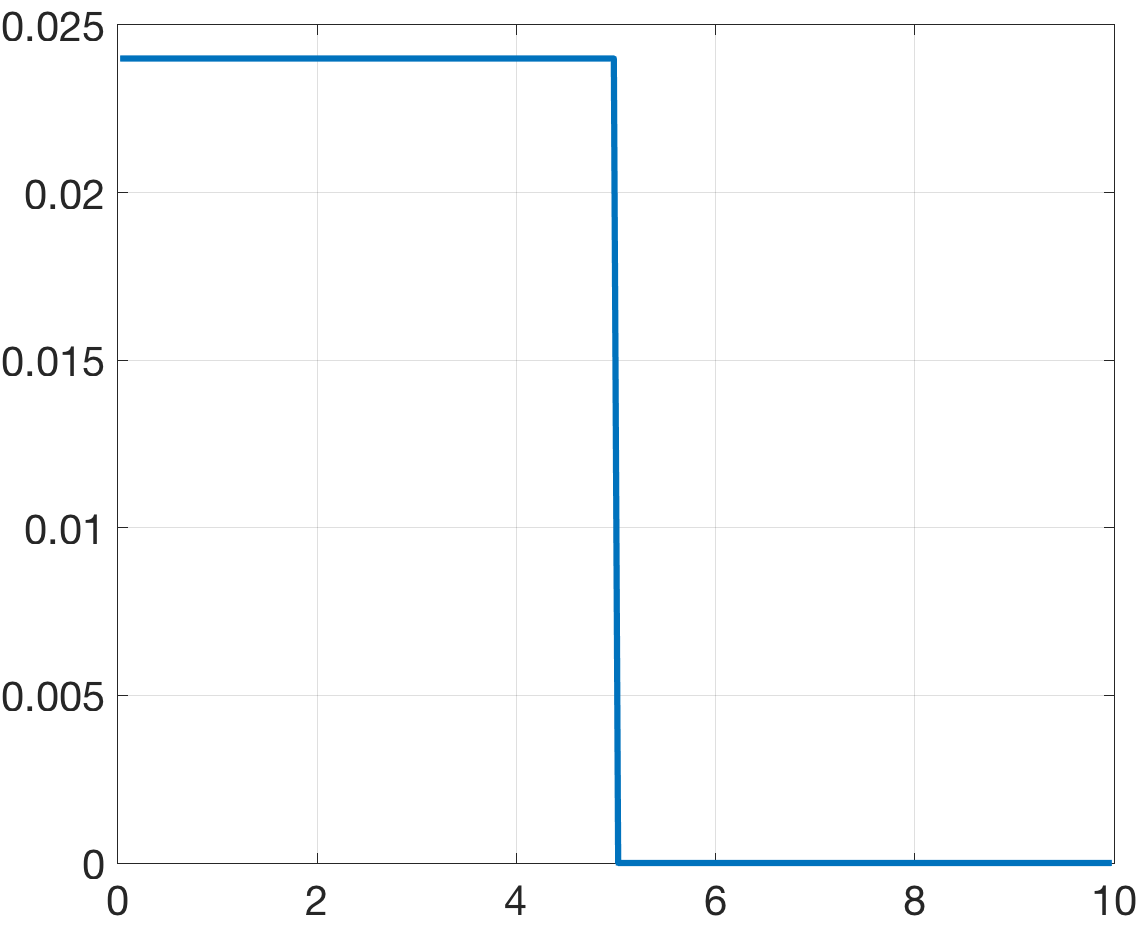
\includegraphics[width=.3\textwidth]{./NumFig/Ini-Mom-2-zoom}
&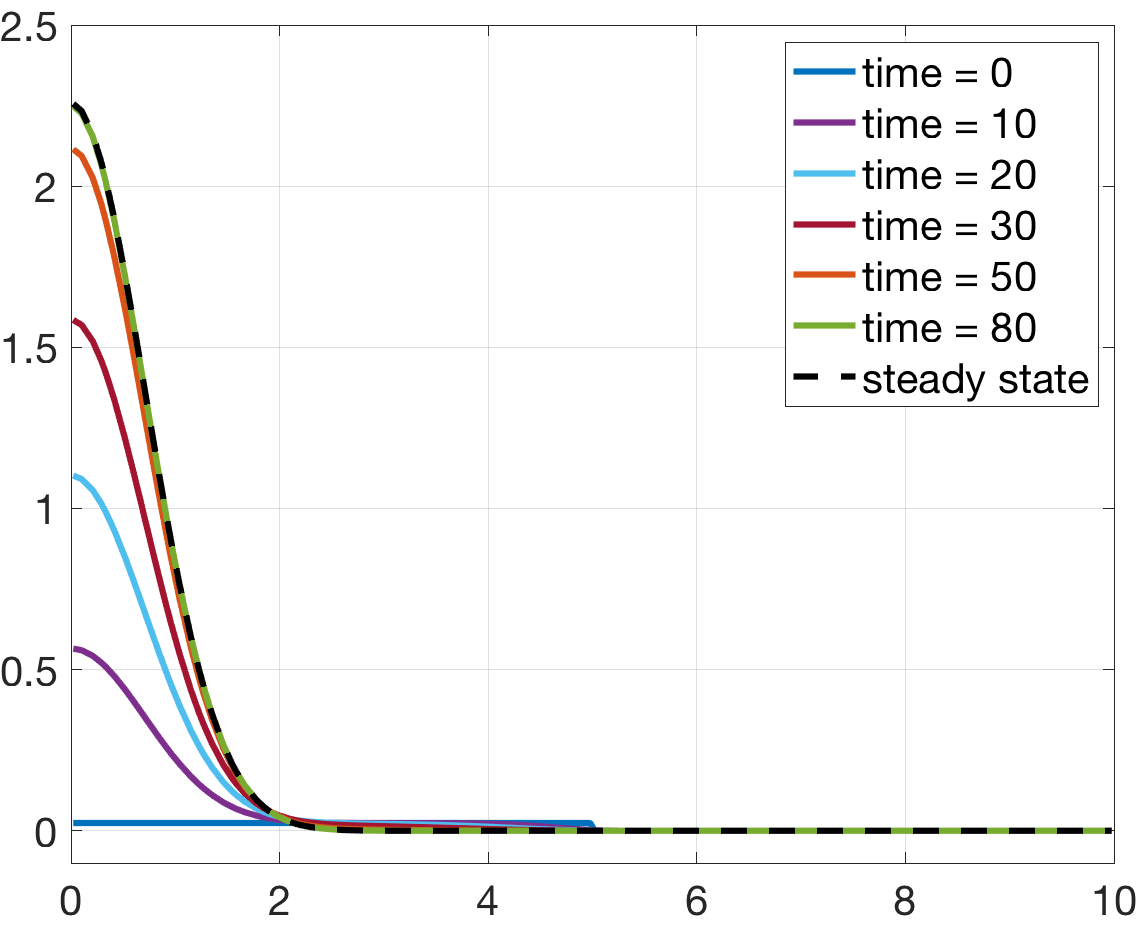
\includegraphics[width=.3\textwidth]{./NumFig/Ini-Mom-2}
&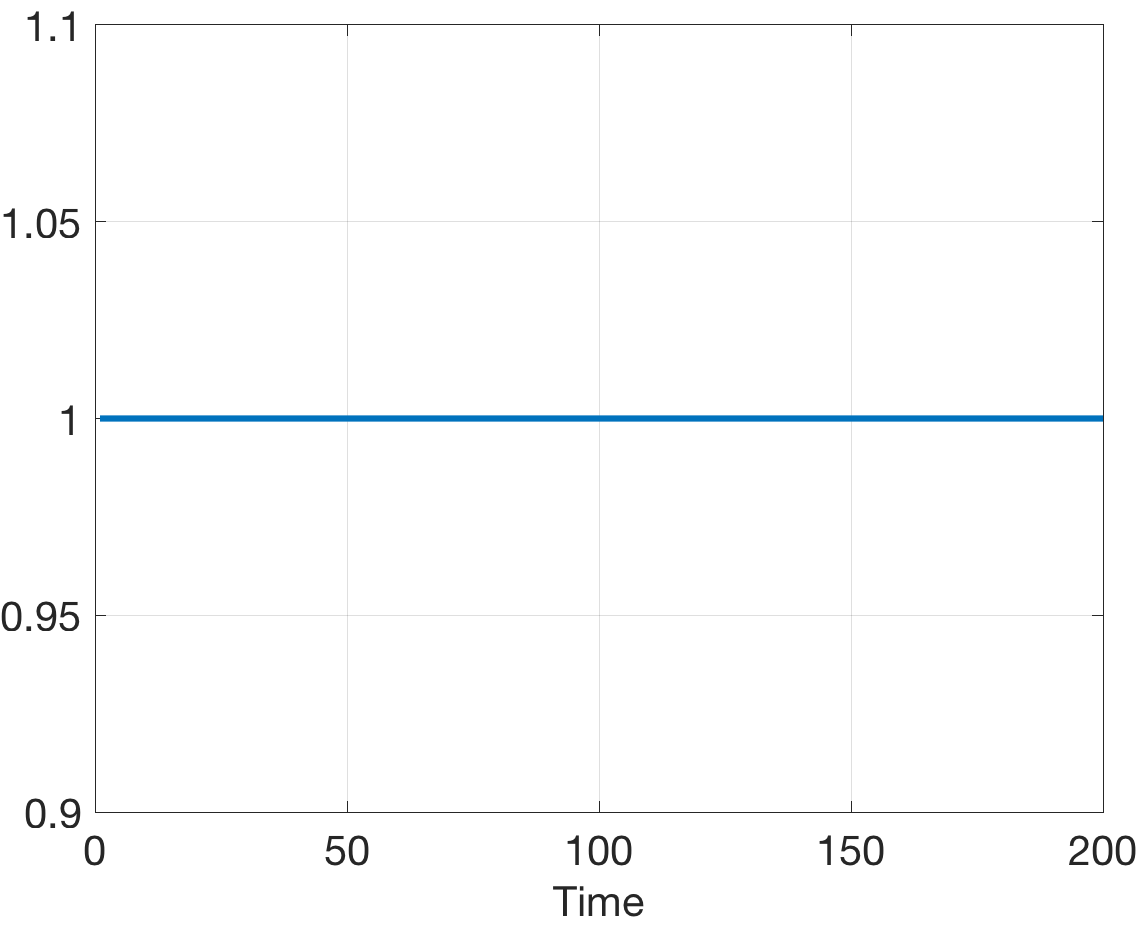
\includegraphics[width=.3\textwidth]{./NumFig/Ini-Mom-2-Conv.png}\\
(a) & (b) & (c)
\end{tabular}
\caption{Test~\ref{Subsec:mom-collisions}b: Plot of numerical solution with upwind flux: (a) plot of initial condition; (b) plot of numerical solution; (c) plot of total mass.}\label{Fig:Mom}
\end{figure}


\subsubsection{Momentum - Electric field acceleration term testing (C=R=0)}


\subsubsection{Momentum - Radiation damping term testing (C=E=0)}


\subsubsection{Complete momentum dynamics}


\subsection{Numerical Scheme for 2D} 


\subsubsection{2D Finite Element Space (Full Grid)}
\label{sec:2d-fe-space}
In two-dimensional simulations, we denote ${\bf n}=(n_1,n_2)\in\mathbb{N}_0^d$ the mesh level for the variables $x_1$ and $x_2$.  We assume the multi-variable is taken as $x_1 = \xi$ and $x_2 = p$ and the mesh $\mathcal{T}_h$ is uniformly dividing into $2^N$ pieces in both the $xi$ and $p$ directions. The grid is constructed by tensor-product, and the elementary cell is defined by 
\begin{equation}
\label{elementarycell}
{\bf I}_{\bf j}^{\bf l}=\{{\bf x}:
x_1\in\big(h_{n_1}j_1,h_{n_1}(j_1+1)\big)\times\big(h_{n_2}j_2,h_{n_2}(j_2+1)\big)\}
\end{equation}
Here ${\bf h}_{\bf n}=(h_{n_1},h_{n_2})$ denotes mesh size in different directions. 
The finite element space is defined by the tensor product rule
\begin{equation}
\label{finiteelementspace}
{\bf V}_k^{\bf n}:=\{v:v(\bx)\in {P}_k({\bf I}_{\bf j}^{\bf n}),0\le{\bf j}\le 2^{\bf n}-1\}=V^{n_1}_{k,x_1}\times V^{n_2}_{k,x_2}
\end{equation}
where $P_k(\bf I_{\bf j}^{\bf n})$ denotes the collection of polynomials of degree up to $k$ in each dimension on cell ${\bf I}_{\bf j}^{\bf n}$. 
Based on a tensor-product construction, the multi-dimensional increment space can be defined as
\begin{eqnarray}
{\bf W}_k^{\bf n}=W_{k,x_1}^{n_1}\times W_{k,x_2}^{n_2}. 
\end{eqnarray}

Furthermore, the full grids finite element space ${\bf V}_k^{N}$ can be represented by
\begin{eqnarray}
{\bf V}_k^{N}=\bigoplus_{0\le n_1\le N, \ 0\le n_2\le N}{\bf W}_k^{\bf n},\text{ where } {\bf n} = (n_1,n_2), \ {\bf n}\in\mathbb{N}_0^d.
\label{Def:FG2D}
\end{eqnarray}
\subsection{Two-Dimensional Model}\label{subsect:2D-scheme}
In this section, we shall develop the numerical scheme for the following two-dimensional model for equation (\ref{fokkerplanckmodel}):
\begin{eqnarray}
-\nabla\cdot\Gamma^C &=& \frac{1}{p^2}\frac{\partial}{\partial p}[p^2C_Ag]  +\frac{1}{p^2}\frac{\partial}{\partial p}[p^2C_Ff]+\frac{1}{p^4}\frac{\partial}{\partial\xi}[C_Bq],\label{eq:2DModel-1}\\ 
-\nabla\cdot\Gamma^E &=&
-\frac{\xi}{p^2}\frac{\partial}{\partial p}[p^2Ef]-\frac{1}{p}\frac{\partial}{\partial\xi}[E(1-\xi^2)f],\label{eq:2DModel-2}\\
-\nabla\cdot\Gamma^R&=&\frac{1-\xi^2}{p^2}\frac{\partial}{\partial p}[\frac{\gamma p^3}{\tau}f ]-\frac{\partial}{\partial\xi}[\frac{\xi(1-\xi^2)}{\gamma\tau}f],\label{eq:2DModel-3}
\end{eqnarray}
where $q = (1-\xi^2)\dfrac{\partial f}{\partial\xi}$ and $g = \dfrac{\partial f}{\partial p}$. The two-dimensional finite element space $\mathcal{V}_h$ can be chosen as full grids finite element space ${\bf V}_k^N$ or sparse grids finite element space $\mathcal{V}_k^N.$ Similar to the previous section, the numerical scheme for two-dimensional model is: find $q_h\in\mathcal{V}_h,\ g_h\in\mathcal{V}_h,\ f_h\in\mathcal{V}_h$, such that,
\begin{eqnarray*}
(q_h,w) &=& \mathcal{D}(f_h,w),\ \forall w\in \mathcal{V}_h, \\
%%%
(g_h,v) &=& \mathcal{G}(f_h,v),\ \forall v\in \mathcal{V}_h,\\
(p^2\frac{\partial f_h}{\partial t},h) &=& \mathcal{C}_1(g_h,h)+\mathcal{C}_2(f_h,h)+\mathcal{C}_3(q_h,h)+\mathcal{E}(f_h,h)+\mathcal{R}(f_h,h), \forall h\in \mathcal{V}_h.
\end{eqnarray*}
On the Cartesian grids, our finite element basis  functions can be rewritten as $w(p,\xi) = w_p(p)w_{\xi}(\xi)$ and $v(p,\xi) = v_p(p)v_{\xi}(\xi)$, and thus the corresponding bilinear forms are defined as:
\begin{eqnarray*}
\mathcal{D}(w,v) &=& 
\sum_{K_p}\int_{K_p}w_pv_pdp\bigotimes\mathcal{D}_{\xi}(w_{\xi},v_{\xi}), \\
%%%
\mathcal{G}(w,v)&=&
\mathcal{G}_{p}(w_p,v_p)\bigotimes\sum_{K_{\xi}}\int_{K_{\xi}}w_{\xi}v_{\xi}d\xi,\\
%%%
\mathcal{C}_1(w,v) &=&
\mathcal{C}_{A,p}(w_p,v_p)\bigotimes\sum_{K_{\xi}}\int_{K_{\xi}}w_{\xi}v_{\xi}d\xi,\\
%%%
\mathcal{C}_2(w,v) &=&
\mathcal{C}_{F,p}(w_p,v_p)\bigotimes\sum_{K_{\xi}}\int_{K_{\xi}}w_{\xi}v_{\xi}d\xi,\\
%%%
\mathcal{C}_3(w,v) &=&
\sum_{K_p}\int_{K_p}\frac{1}{p^2}w_pv_pdp\bigotimes\mathcal{C}_{B,\xi}(w_{\xi},v_{\xi}),\\
%%%
\mathcal{E}(w,v) &=& 
\mathcal{E}_{p}(w_p,v_p)\bigotimes\sum_{K_{\xi}}\int_{K_{\xi}}\xi w_{\xi}v_{\xi}d\xi+\sum_{K_{p}}\int_{K_{p}}p w_{p}v_{p}dp\bigotimes\mathcal{E}_{\xi}(w_{\xi},v_{\xi}),\\
%%%
\mathcal{R}(w,v)&=&\frac{1}{\tau}\mathcal{R}_p(w_p,v_p)\bigotimes\sum_{K_{\xi}}\int_{K_{\xi}}(1-\xi^2)w_{\xi}v_{\xi}d\xi-\frac{1}{\tau}\sum_{K_p}\int_{K_p}p^2w_pv_pdp\bigotimes\mathcal{R}_{\xi}(w_{\xi},v_{\xi}).
\end{eqnarray*}
In the above bilinear forms, $\bigotimes$ denotes the Kronecker product. 


\subsubsection{Full-Grid Relaxation to Maxwellian test}
\label{sec:fg-relaxation}
As a starting point, we will assume a time-independent plasma density and temperature: 
\bq
{\tilde T}=T \, , \qquad {\tilde n}=n \, ,
\eq
which implies:
\bq
 \bar{\nu}_{ee}=1 \, , \qquad \bar{v}_T=1 \, .
 \eq

 
\subsection{Collision Term $\Gamma^C$}
\label{sec:FullModel-1}
%
In this section, we shall consider the flux associated with collisions, $\Gamma^c$, and the equation is described as follows:
\begin{eqnarray}
\frac{\partial f}{\partial t} = \frac{1}{{ p}^2}\frac{\partial}{\partial { p}}\bigg({ p}^2C_A\frac{\partial f}{\partial { p}}\bigg) + \frac{1}{{ p}^2}\frac{\partial}{\partial { p}}\bigg({ p}^2C_F f\bigg)+\frac{1}{{ p}^4}\frac{\partial}{\partial\xi}\bigg(C_B(1-\xi^2)\frac{\partial f}{\partial\xi}\bigg).
\label{2DMomentumEqn}
\end{eqnarray}

\noindent{\bf Test~\ref{sec:FullModel-1}.}
For this test, we set the model parameters as:% $\delta$, $Z$, $\hat{\tau}$, and $\hat{E}$.
 %
\bq
\delta=0.042 \, , \qquad Z=1 \, , \qquad {\hat E}=0.0025 \, , \qquad \hat{\tau}=10^5 \, ,
\eq
with integration time $t_{max}=10^3$, and let domain $\xi\times {p}\in [-1,1]\times[0,10]$.
For the initial condition we will take a Maxwellian distribution:
%
\bq
f= \frac{2}{\sqrt \pi} e^{-{p}^2} \, , \qquad \int_{-1}^1\,  d \xi  \int_{0}^\infty \, f \, {p}^2 \, d {p} =1.  
\eq
The boundary conditions are: Neumann boundary for $\xi$ and:
\begin{eqnarray*}
\left. \frac{\partial f}{\partial {p}}\right|_{ {p}=0}=0 \, , \qquad f( {p}=10,t)=0
\end{eqnarray*}

In the following numerical simulation, we shall employ the alternating flux.

\noindent{\bf Test~\ref{sec:FullModel-1}a}
The initial condition is chosen as
\begin{eqnarray}
f_0(\xi,{p},t=0) = \begin{cases}
\dfrac{3}{2\cdot5^3}, \text{ if }0\le {p}\le5,\\
0, \hspace{1.5cm} \text{ else}.
\end{cases}\label{NumTest6-1}
\end{eqnarray}

\begin{figure}[H]
\centering
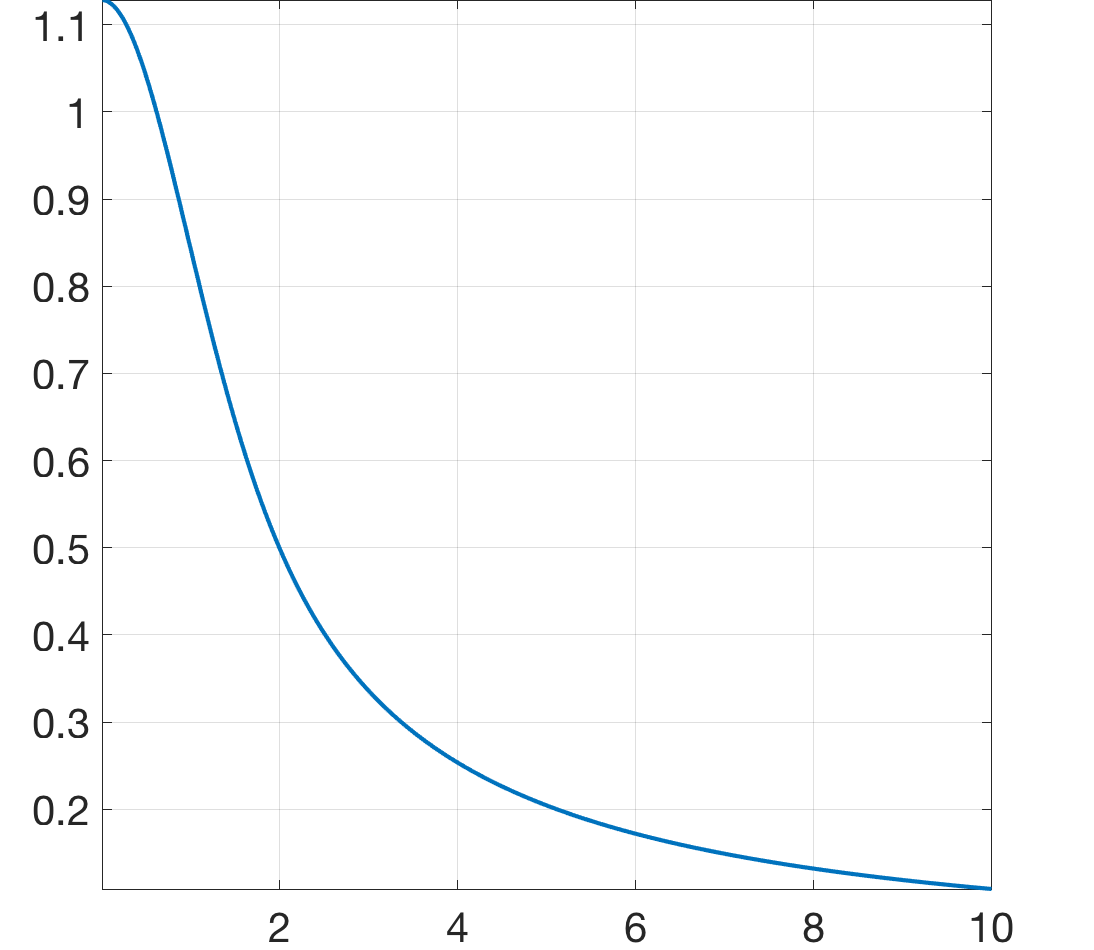
\includegraphics[width=.32\textwidth]{./NumFig/FullModel-Ca}
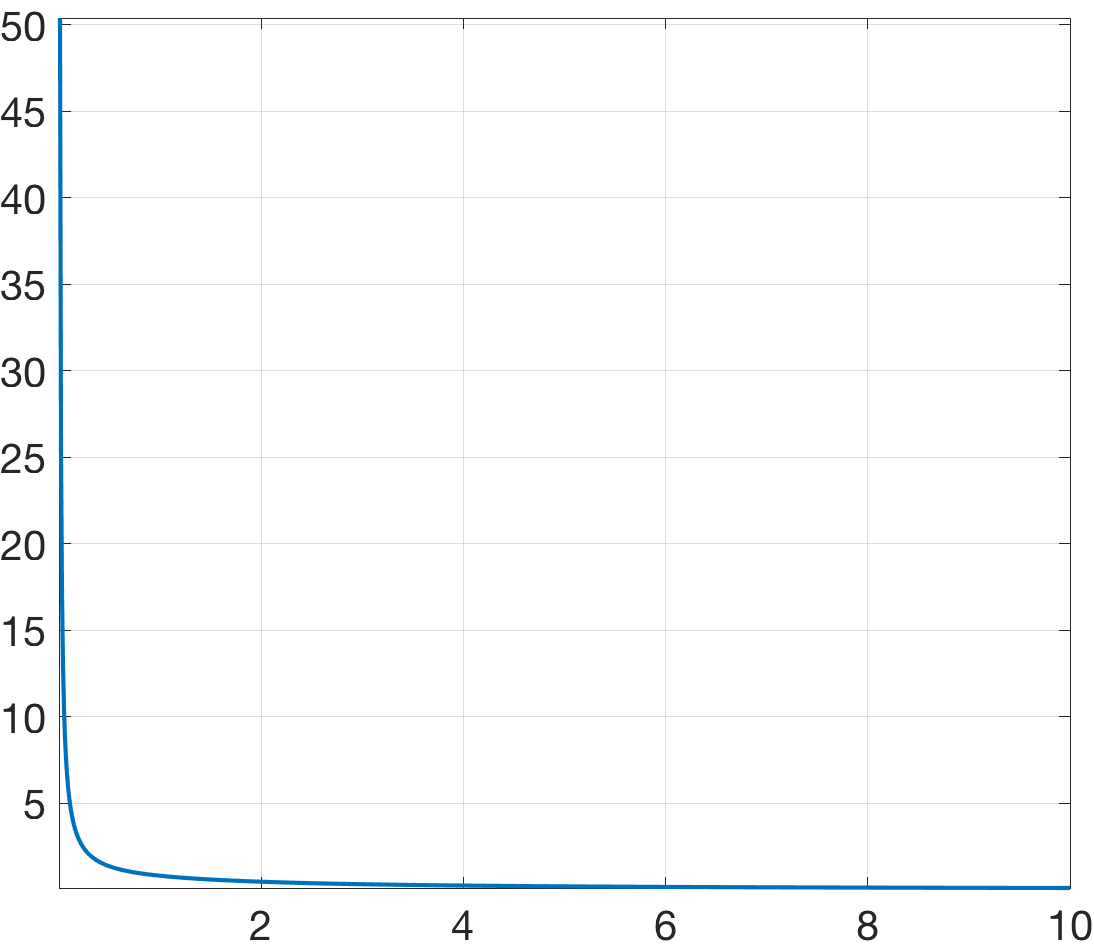
\includegraphics[width=.32\textwidth]{./NumFig/FullModel-Cb}
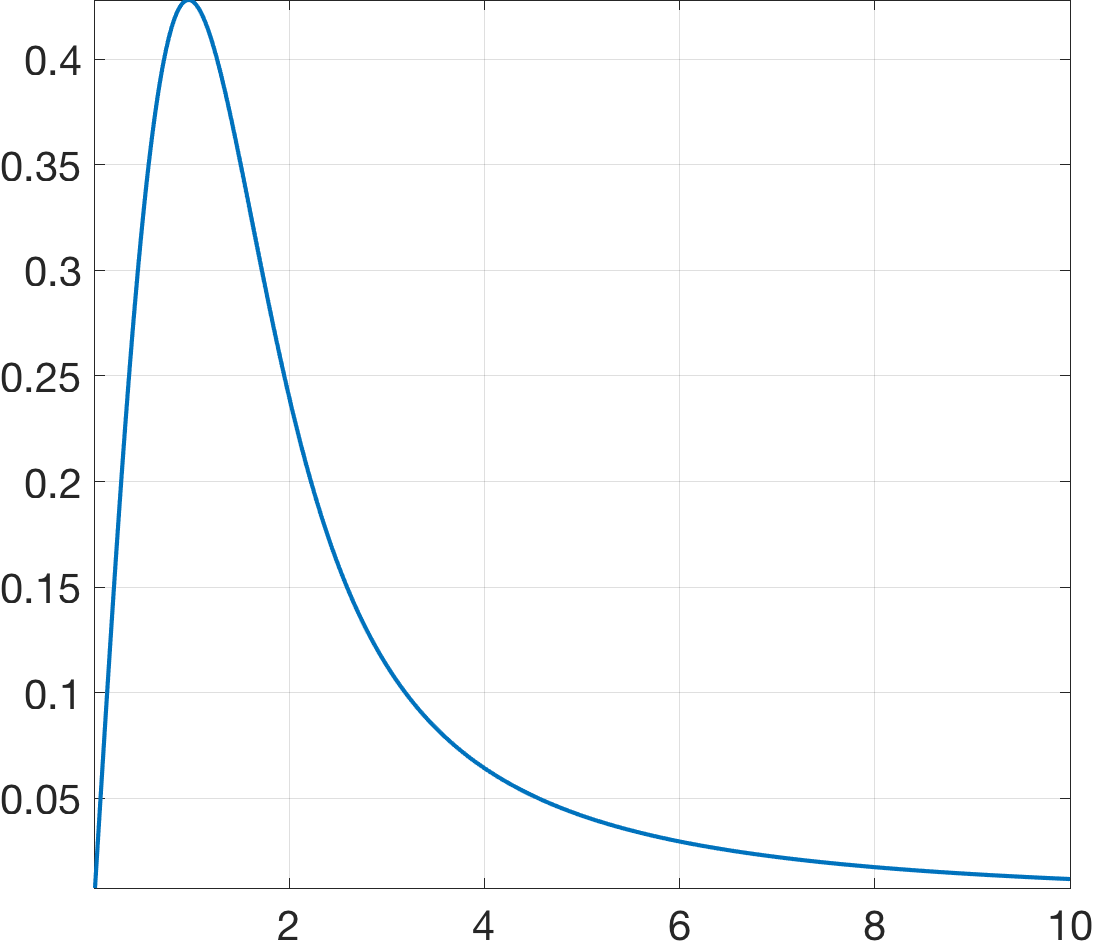
\includegraphics[width=.32\textwidth]{./NumFig/FullModel-Cf}
\caption{Test~\ref{sec:FullModel}: Plot of coefficients $C_A$ (left), $C_B$ (middle), and $C_F$ (right).}
\end{figure}

Figure~\ref{Fig:NumTest6-1-1} plots the numerical solution at the mesh with $N$ = $5$, $k=1$. At $t=0$, the solution is step function in ${p}$. 

\begin{figure}[H]
\centering
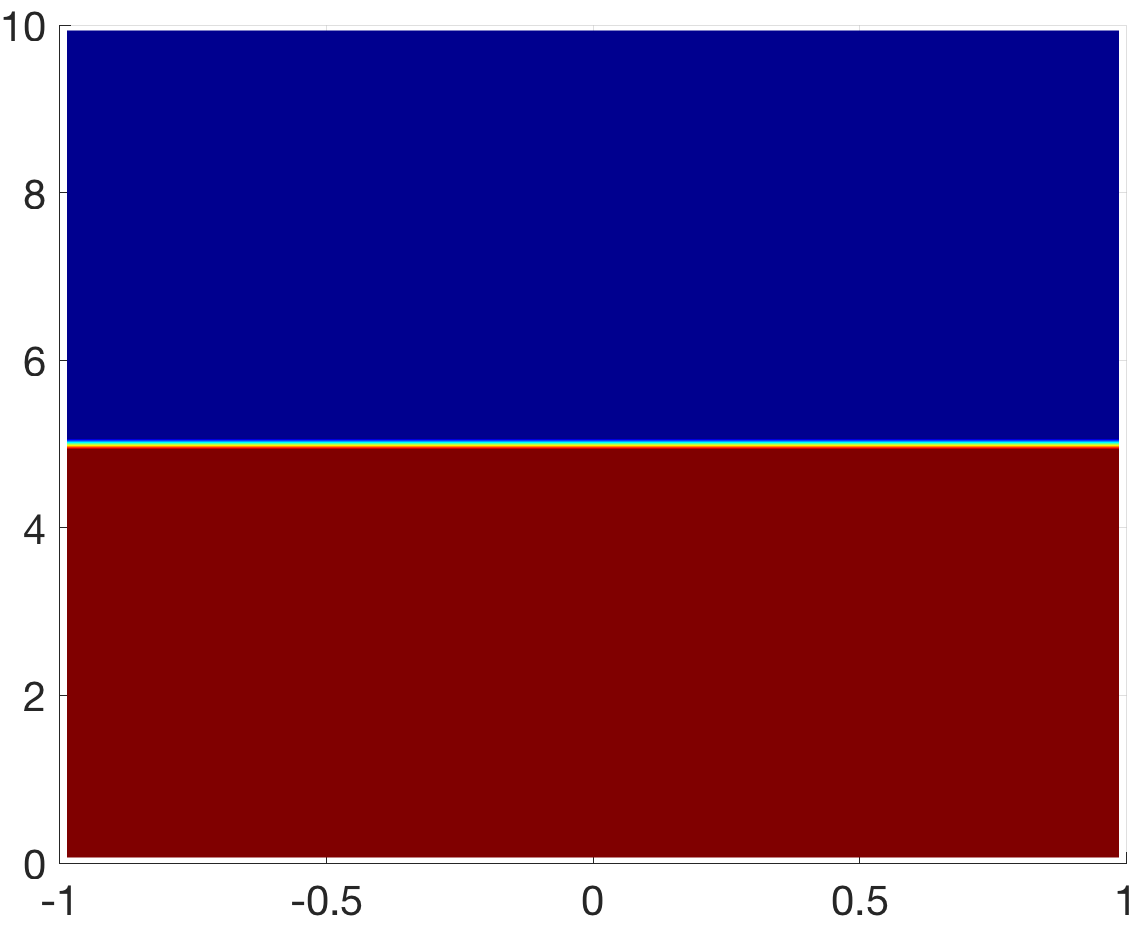
\includegraphics[width=.3\textwidth]{./NumFig/FullModel2D-1-Ini}
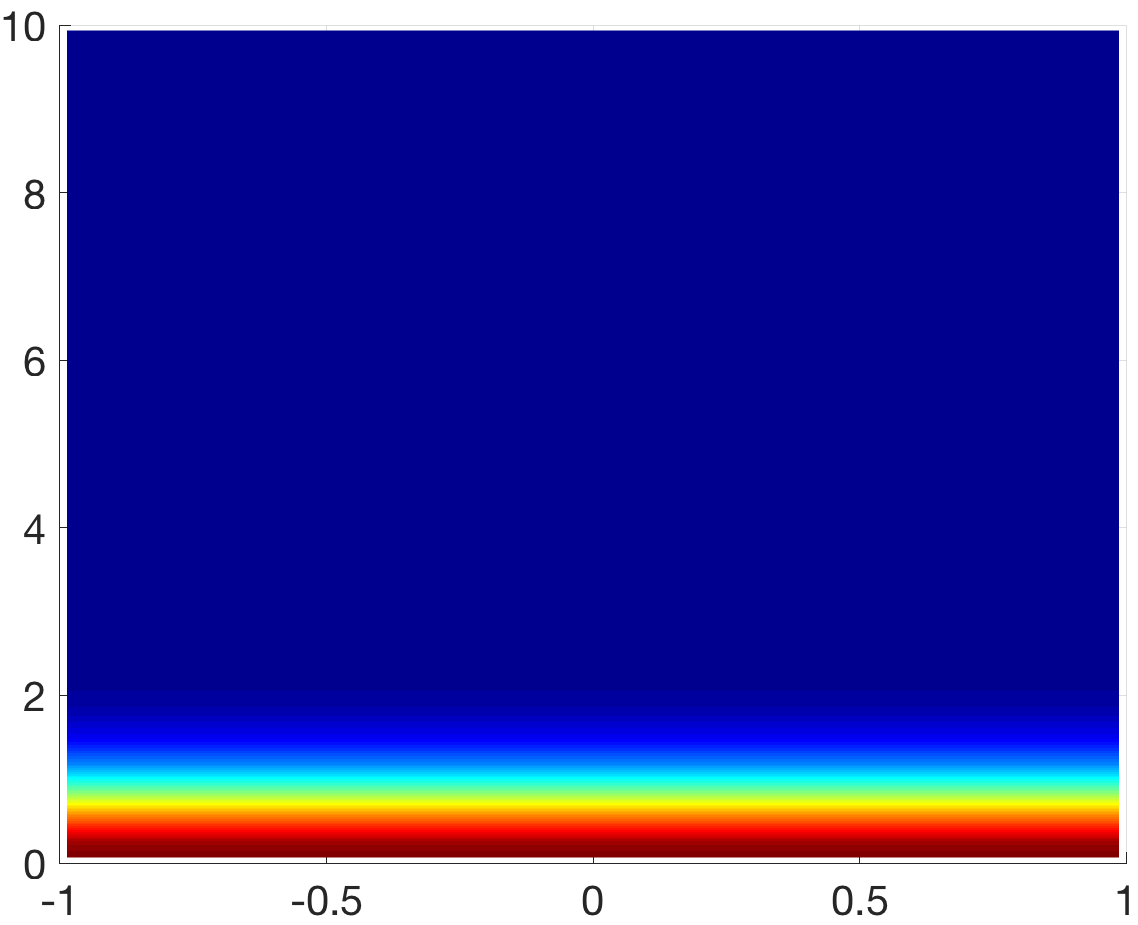
\includegraphics[width=.3\textwidth]{./NumFig/FullModel2D-1-100}
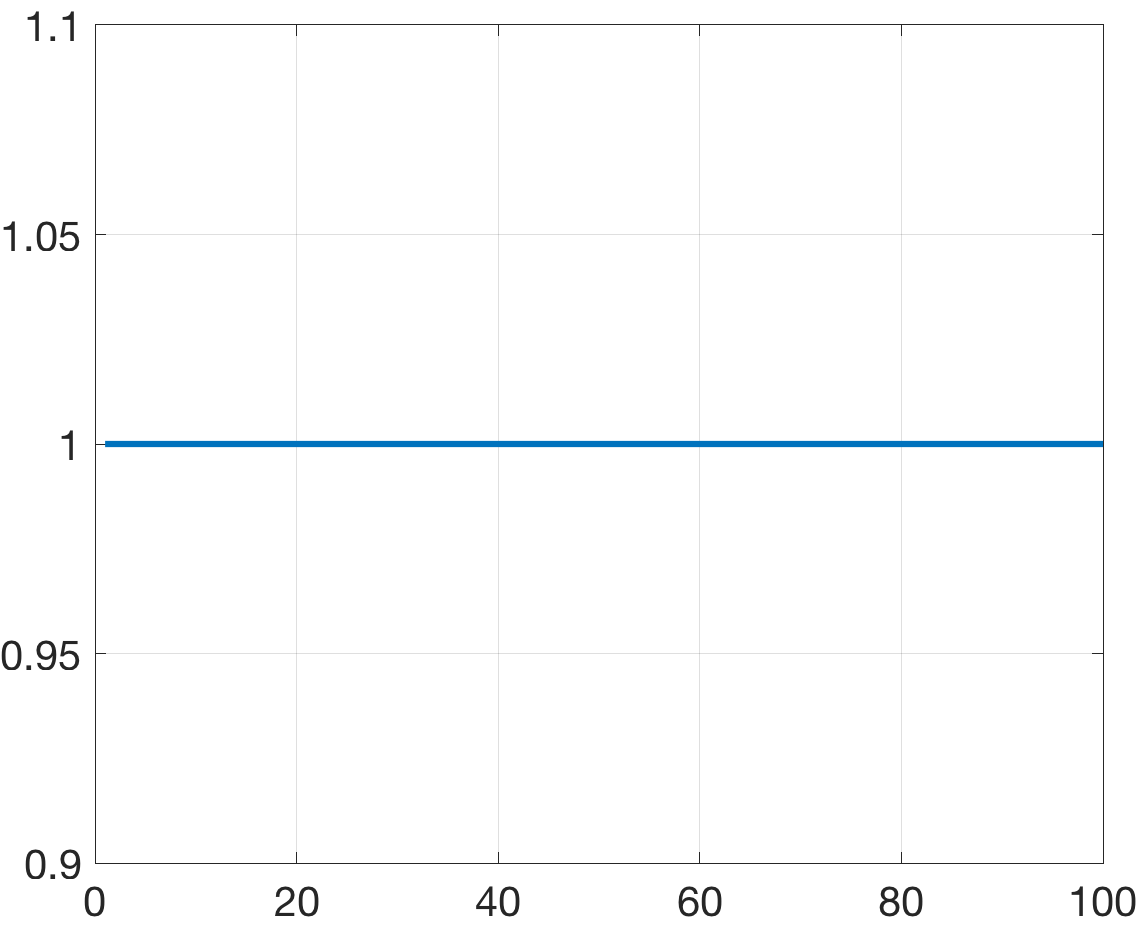
\includegraphics[width=.3\textwidth]{./NumFig/FullModel2D-1-Conv}
\caption{Test~\ref{sec:FullModel-1}a: Plot of initial condition (\ref{NumTest6-1}) (left), solution at time $= 100$ (middle), and conservation property (right).}\label{Fig:NumTest6-1-1}
\end{figure}

\noindent{\bf Test~\ref{sec:FullModel-1}b}
The initial condition is chosen as
\begin{eqnarray}
f_0(\xi,{p}) = \frac{2}{\sqrt{\pi}a^3}\exp(-{p}^2/a^2), \text{ with } a = 2.\label{NumTest6-2}
\end{eqnarray}

\begin{figure}[H]
\centering
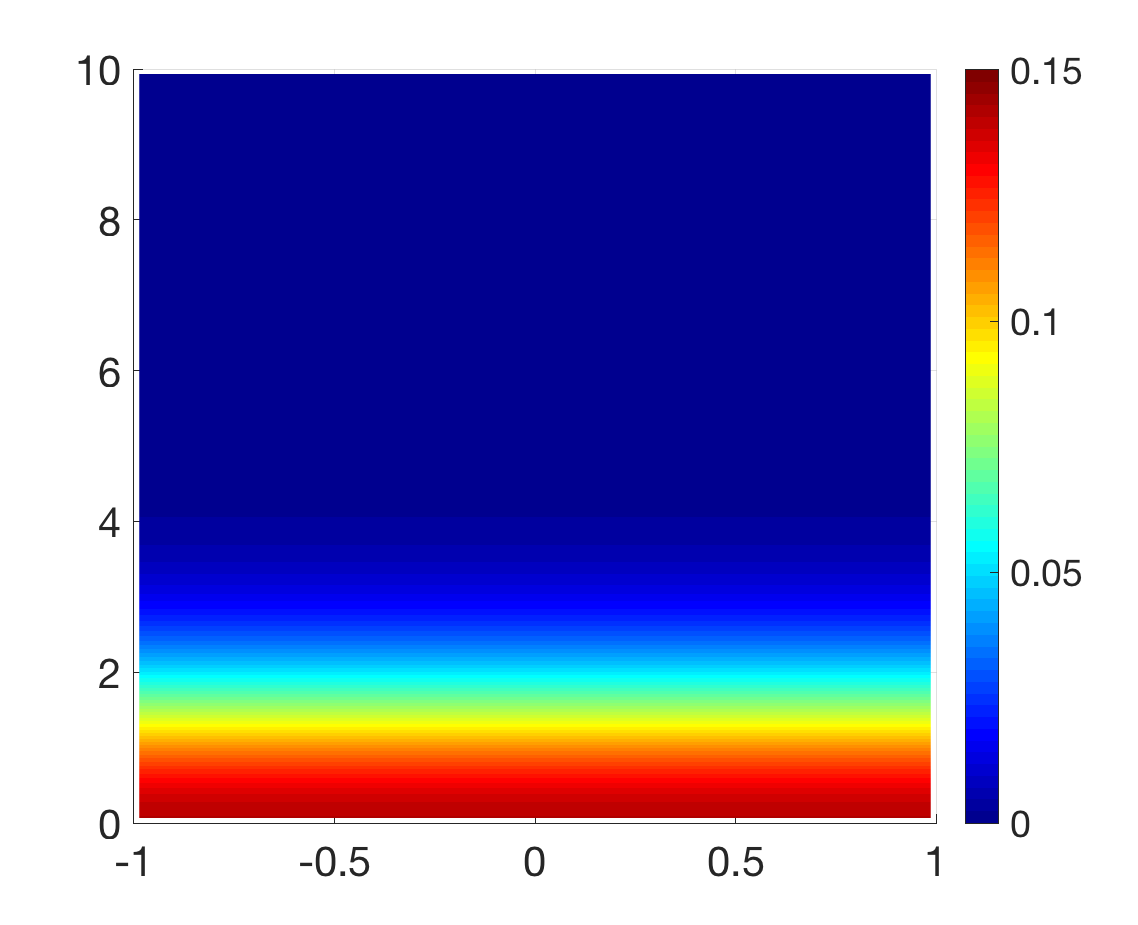
\includegraphics[width=.32\textwidth]{./NumFig/FullModel2D-2-Ini}
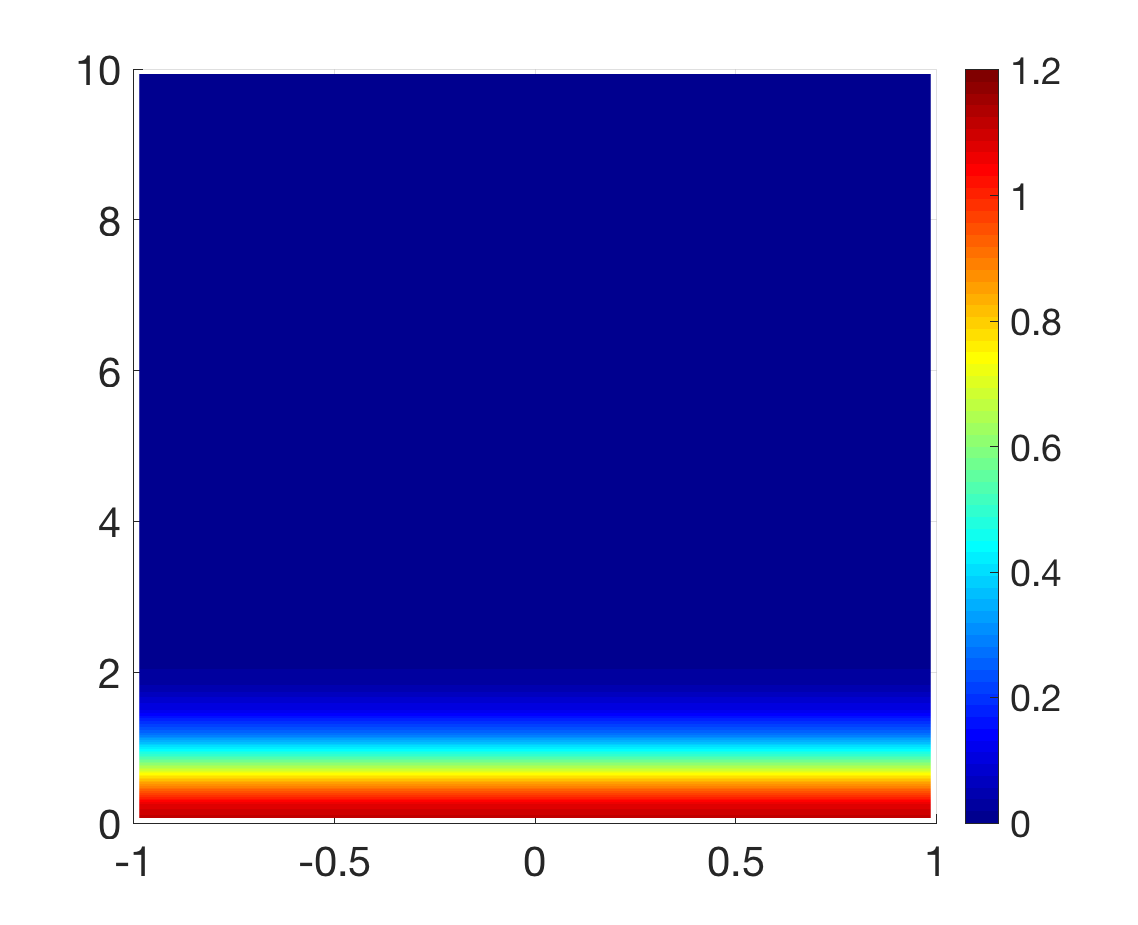
\includegraphics[width=.32\textwidth]{./NumFig/FullModel2D-2-100}
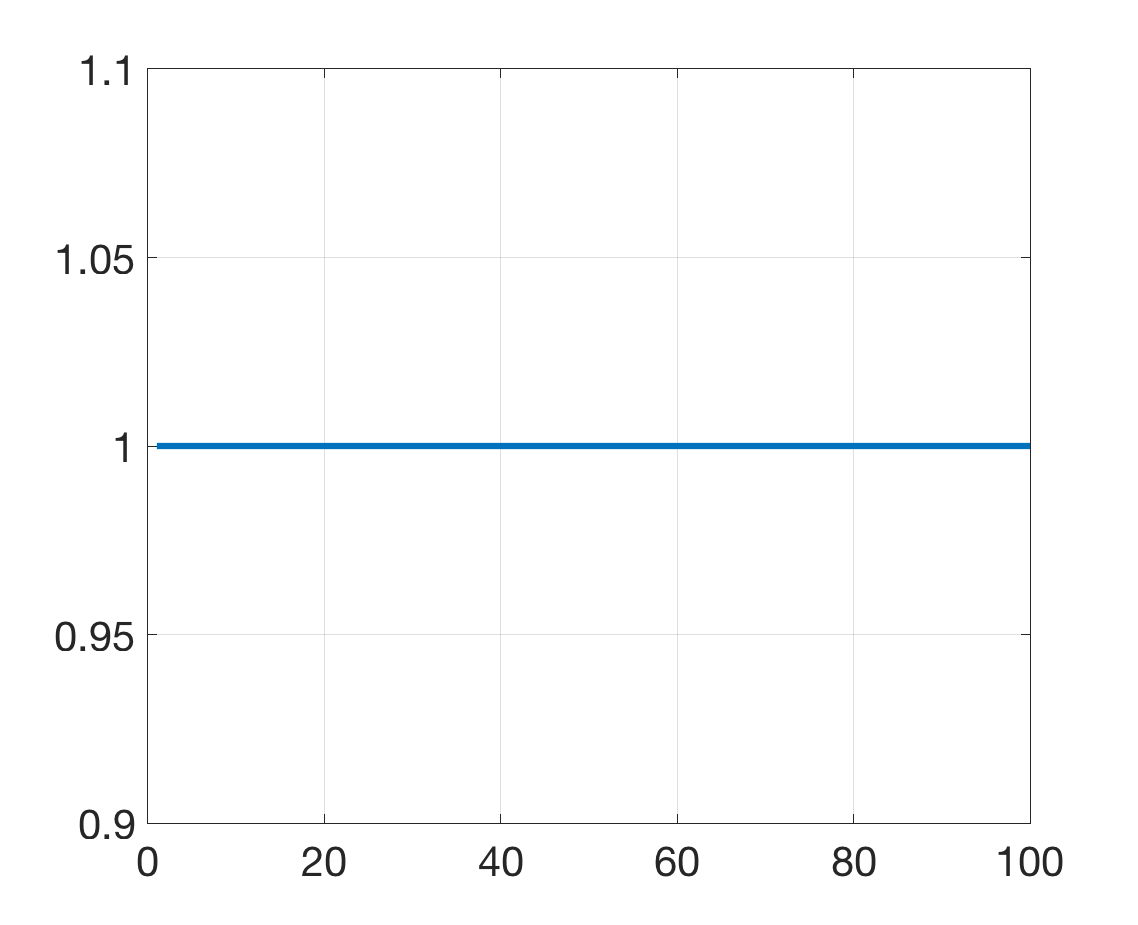
\includegraphics[width=.32\textwidth]{./NumFig/FullModel2D-2-Conv}
\caption{Test~\ref{sec:FullModel-1}b: Plot of initial condition (\ref{NumTest6-2}) (left), solution at time $= 100$ (middle), and conservation property (right).}
\end{figure}

\noindent{\bf Test~\ref{sec:FullModel-1}c}
The initial condition is chosen as 
\begin{eqnarray}
 f_0(\xi,{p})=\bigg(\sum_{L=0}^6 h_L P_L(\xi)\bigg) \bigg(\frac{2}{3\sqrt{\pi}}\exp(-{p}^2)\bigg), \label{NumTest6-3}
\end{eqnarray}
with $h_0 = 3, h_1=0.5, h_2 = 1, h_3 = 0.7, h_4 = 3, h_5 = 0, h_6 = 3$ and $P_L$ as Legendre polynomial.

\begin{figure}[H]
\centering
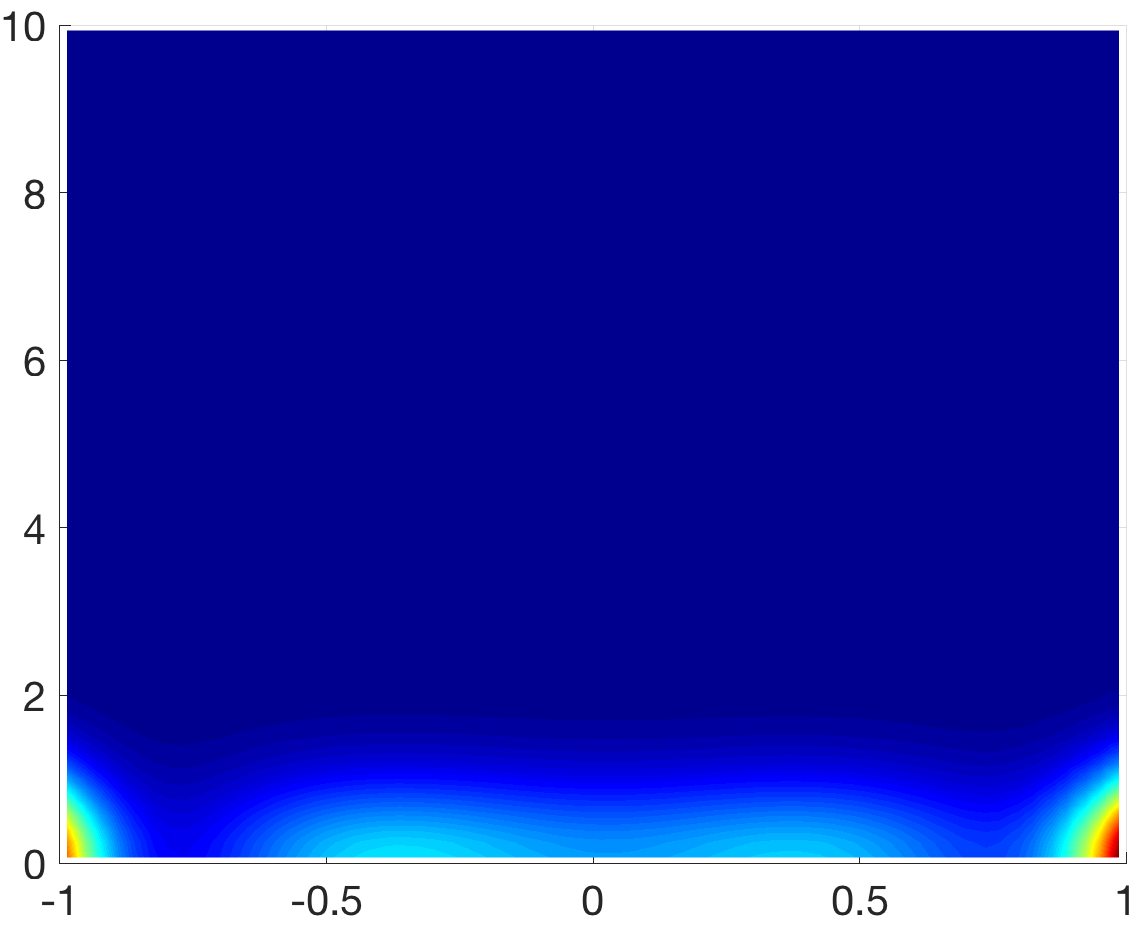
\includegraphics[width=.32\textwidth]{./NumFig/FullModel2D-3-1}
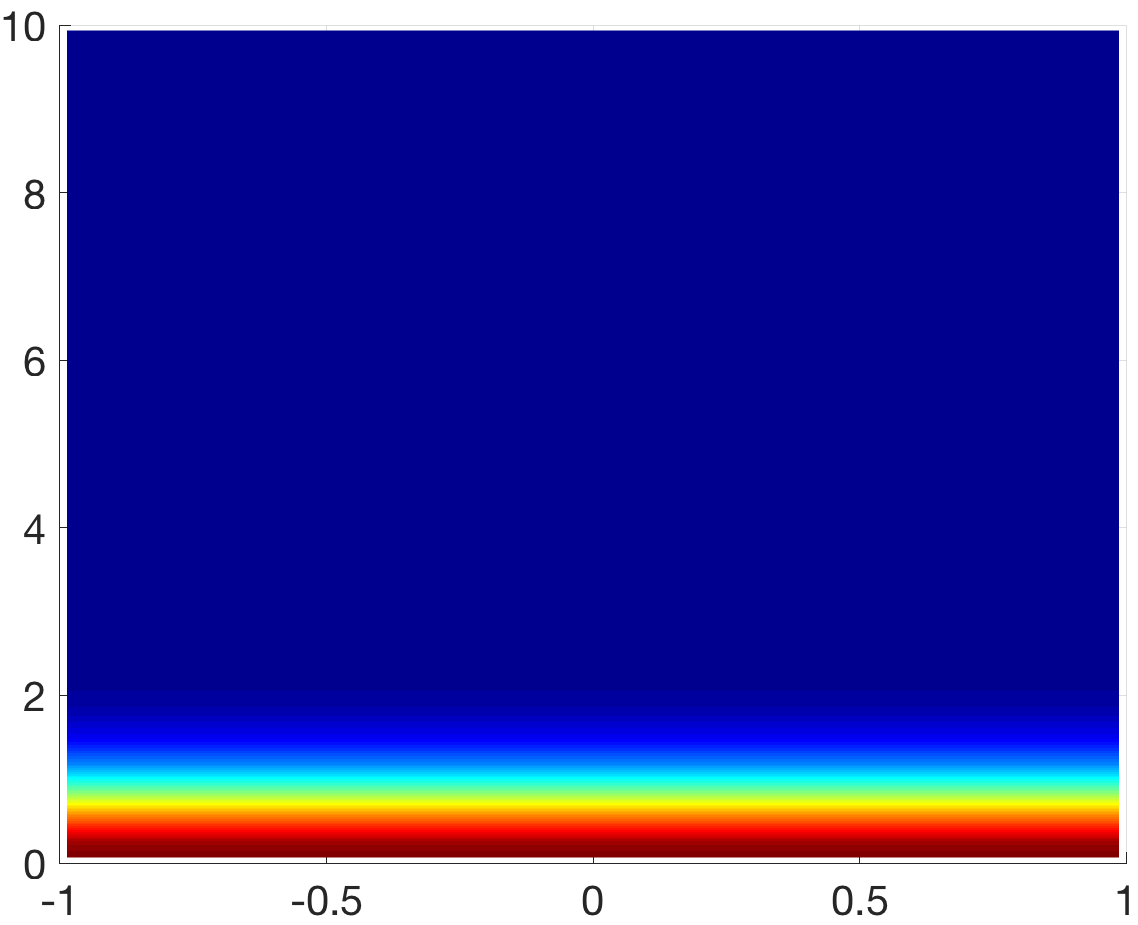
\includegraphics[width=.32\textwidth]{./NumFig/FullModel2D-3-100}
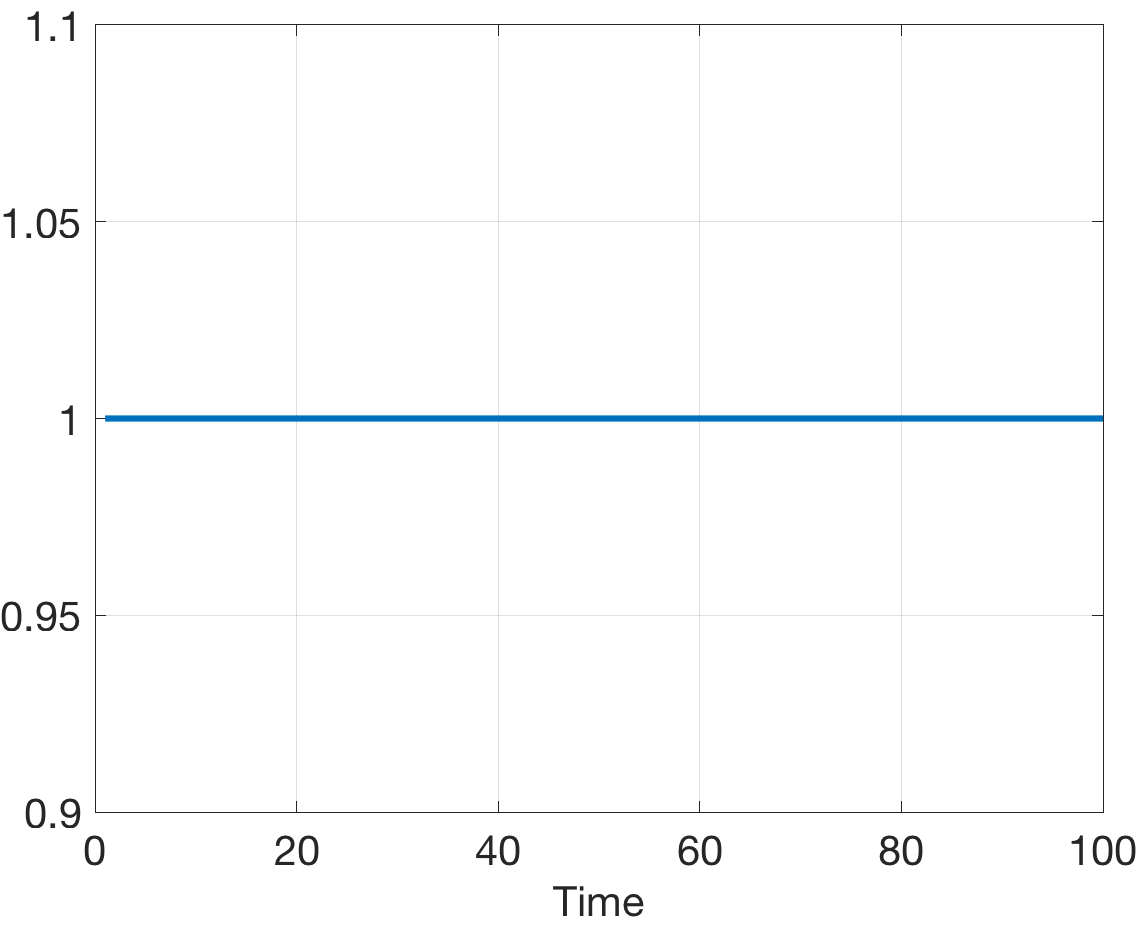
\includegraphics[width=.32\textwidth]{./NumFig/FullModel2D-3-conv}
\caption{Test~\ref{sec:FullModel-1}c: Plot of initial condition (\ref{NumTest6-3}) (left), solution at time $= 100$ (middle), and conservation property (right).}
\end{figure}

\noindent{\bf Test~\ref{sec:FullModel-1}d}
The initial condition is chosen as 
\begin{eqnarray}
 f_0(\xi,\hat{p})=\bigg(1-\frac{1}{2}\sin(\pi \xi)\bigg) \bigg(\frac{2}{\sqrt{\pi}}\exp(-\hat{p}^2)\bigg), \label{NumTest6-4}
\end{eqnarray}

\begin{figure}[H]
\centering
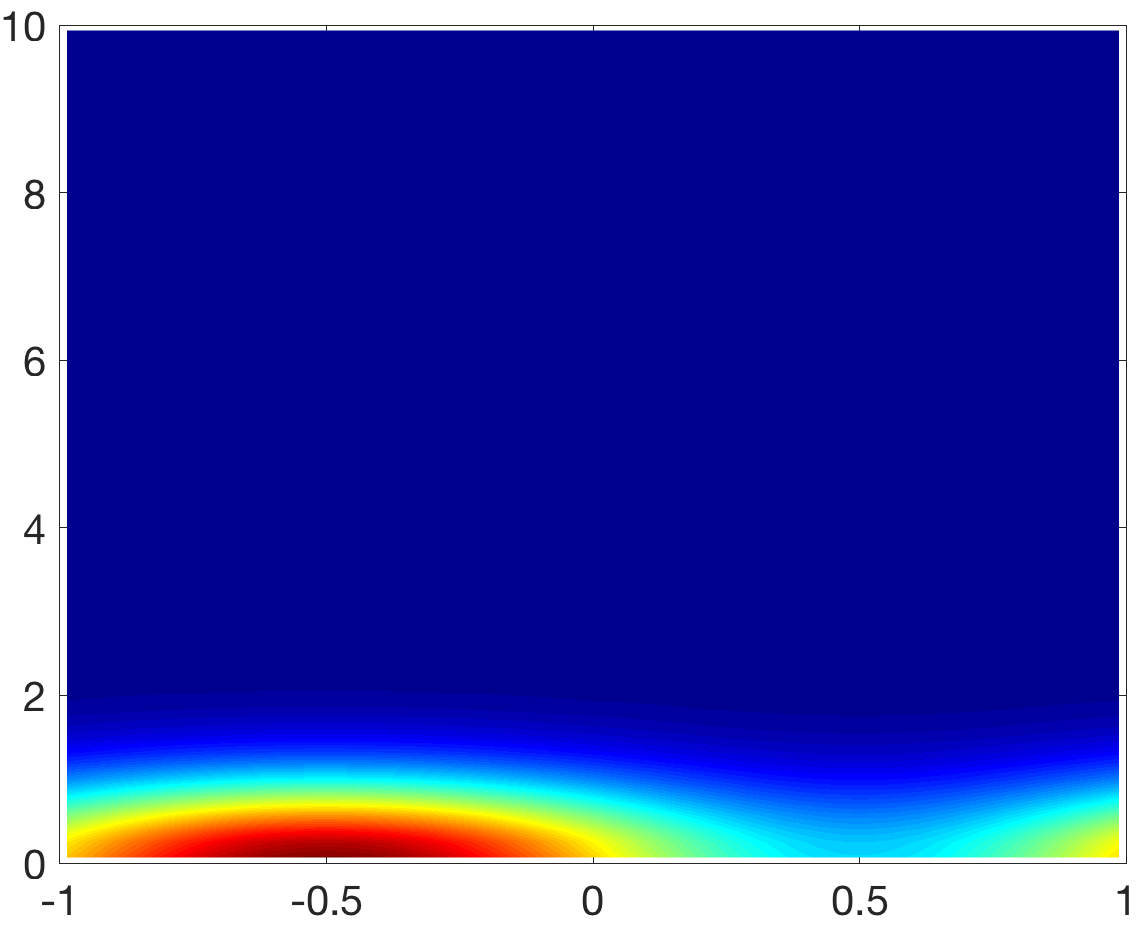
\includegraphics[width=.32\textwidth]{./NumFig/FullModel2D-4-0}
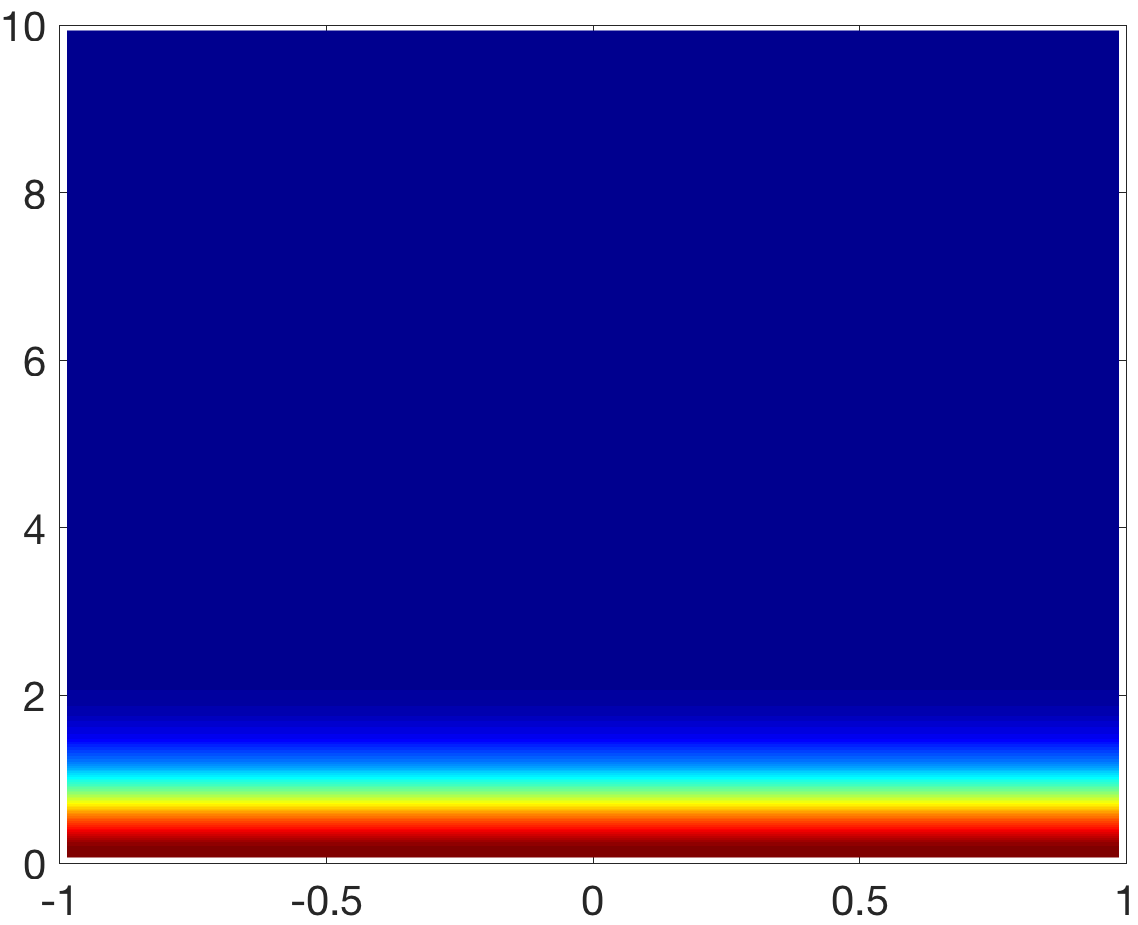
\includegraphics[width=.32\textwidth]{./NumFig/FullModel2D-4-100}
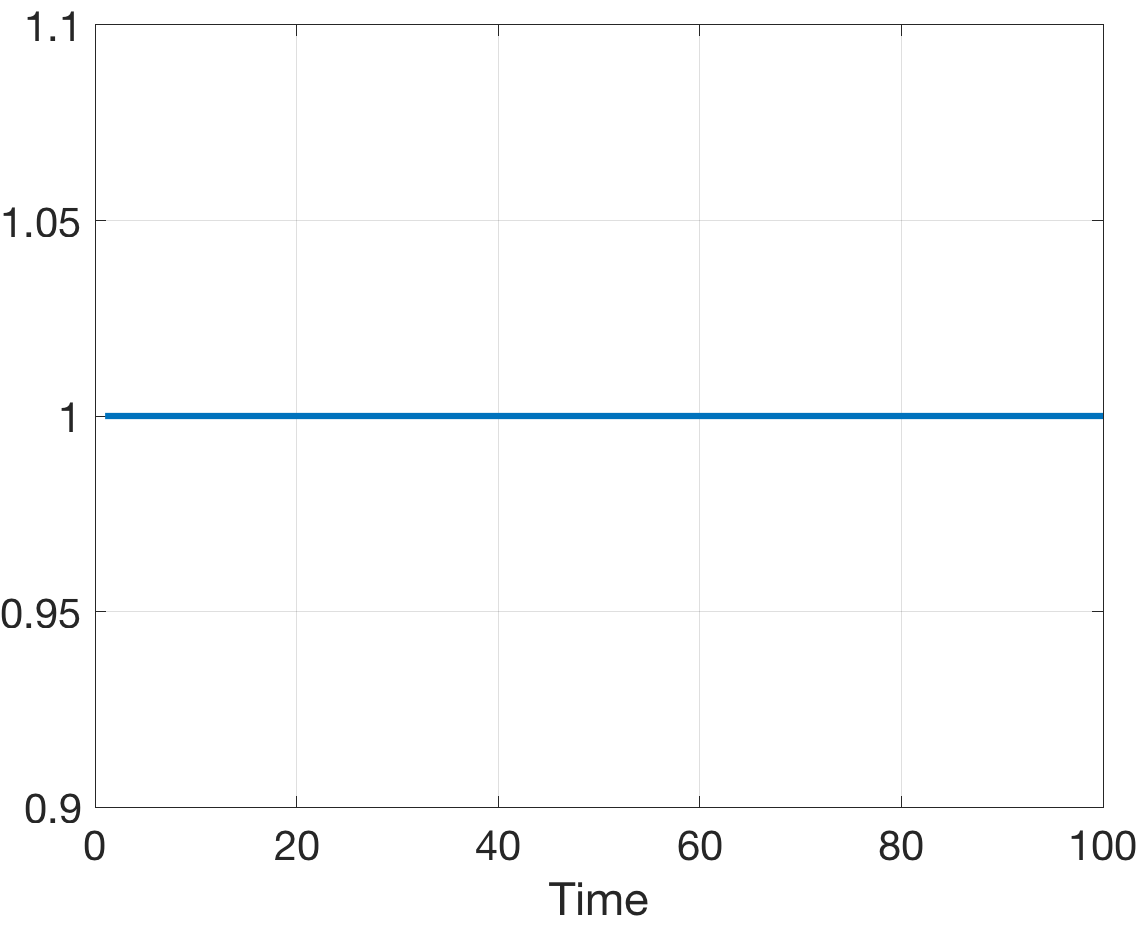
\includegraphics[width=.32\textwidth]{./NumFig/FullModel2D-4-conv}
\caption{Test~\ref{sec:FullModel-1}d: Plot of initial condition (\ref{NumTest6-4}) (left), solution at time $= 100$ (middle), and conservation property (right).}
\end{figure}


\subsubsection{Full-Grid Runaway production rate test}
\label{sec:FullModel-2}
- Notes on the production rate test \todo{**DIEGO**}
In this section, let the computational domain as $[-1,1]\times[0,20]$ and we shall approximate the numerical solution to equation (\ref{eq:2DModel-1})-(\ref{eq:2DModel-3}). In the implementation of our algorithm, the upwind flux will be employed other than the collision operator; the collision operator will use alternation flux to approximate. 
In the following tests, we shall define the following mass functions:
\begin{eqnarray}
    \text{Total Mass: }M_1&=&\int_{0}^{20} \int_{-1}^1 p^2 f \ dp \ d\xi;\label{eq:totalmass}\\
    \text{Leaking Mass: }M_2&=&\int_{p_\text{cutoff}}^{20} \int_{-1}^1 p^2 f \ dp \ d\xi,\label{eq:leakingmass}
\end{eqnarray}
where $p_\text{cutoff}$ is a chosen cutoff value for momentum variable $p.$

\noindent{\bf Test \ref{sec:FullModel-2}}
We shall choose the following Maxwellian distribution as the initial condition
\begin{equation*}
    f_0(\xi,p) = Q\exp(-\frac{2}{\delta^2}\sqrt{1+\delta^2p^2}),
\end{equation*}
where $Q$ is a constant such that $\int\int p^2 f_0 \ d\xi \ dp = 1$. In the practical computation, the high order numerical integration approach is applied to compute $Q$ for different values of $\delta$.

\vskip.1in
The initial condition is plotted in Fig~\ref{fig:delta} for different values of $\delta$. By comparing the initial data with Gaussian distribution function $\frac{2}{\sqrt{\pi}}\exp(-p^2)$, we see that larger values of $\delta$ induce an initial function differing more from a Gaussian function.

\begin{figure}[H]
    \centering
    \includegraphics[width=.5\textwidth]{./Fig_2D/f0-deltav2}
    \caption{Illustration of initial state for $f_0$ with different values in $\delta$.}
    \label{fig:delta}
\end{figure}

{\bf Test \ref{sec:FullModel-2}a}
The first test is to check the performance of the numerical solution. Let $\delta = 0.3$, $E = 0.4,\; Z = 5$, and denote: 
$$
p_{\parallel} = p\xi,\quad
p_{\perp} = p\sqrt{1-\xi^2}.
$$
The numerical solutions and contour plots at different time period are illustrated in Fig~\ref{fig:sol@time} and Fig~\ref{fig:sol@contour}. It can be observed that the magnitude of the numerical solution is decreasing and the long tails are developed with time involving.

\begin{figure}[H]
    \centering
    \includegraphics[width=.32\textwidth]{Fig_2D/T1plotPen}
    \includegraphics[width=.32\textwidth]{Fig_2D/T2plotPen.png}
    \includegraphics[width=.32\textwidth]{Fig_2D/T3plotPen.png}\\
    \includegraphics[width=.32\textwidth]{Fig_2D/T4plotPen}
    \includegraphics[width=.32\textwidth]{Fig_2D/T5plotPen.png}
    \includegraphics[width=.32\textwidth]{Fig_2D/T6plotPen.png}
    \caption{Test \ref{sec:FullModel-2}a: Numerical solutions at different time period.}
    \label{fig:sol@time}
\end{figure}

\begin{figure}[H]
    \centering
    \includegraphics[width=.32\textwidth]{Fig_2D/T1Contour}
    \includegraphics[width=.32\textwidth]{Fig_2D/T2Contour}
    \includegraphics[width=.32\textwidth]{Fig_2D/T3Contour}\\
    \includegraphics[width=.32\textwidth]{Fig_2D/T4Contour}
    \includegraphics[width=.32\textwidth]{Fig_2D/T5Contour}
    \includegraphics[width=.32\textwidth]{Fig_2D/T6Contour}
    \caption{Test \ref{sec:FullModel-2}a: Contour plot for numerical solutions at different time period.}
    \label{fig:sol@contour}
\end{figure}

Mass conservation is verified in Fig~\ref{fig:MassPlot}.
It is interesting to see that the mass ($M_1$ defined in (\ref{eq:totalmass})) is perfectly conserved up to $t = 50$. The leaking mass ($M_2$), which is defined in (\ref{eq:leakingmass}), is also plotted in this figure. One can observe that $M_2$ is almost zero when $t<10$ due to the initial state almost vanishing for $p>10$. As time passes, $M_2$ is increasing until $t = 50$. Actually, the quantity of $M_2$ will be increased to its maximum and then begins to drop. 
\begin{figure}[H]
    \centering
    \includegraphics[width=.5\textwidth]{Fig_2D/MassPlot}
    \caption{Test \ref{sec:FullModel-2}a: Plot of Mass at different time period}
    \label{fig:MassPlot}
\end{figure}

{\bf Test \ref{sec:FullModel-2}b} 
By setting $\delta = 0.3$, $p_\text{cutoff} = 10$, and choosing different values in $E$ and $Z$, our approach has been applied to test the maximum value of $M_2$. 
\begin{figure}[H]
    \centering
    \includegraphics[width=.5\textwidth]{./Fig_2D/Rate-Del3e-1}
    \caption{Test \ref{sec:FullModel-2}b: Maxmium of $M_2$ for different values in $Z$.}
    \label{fig:maxM2}
\end{figure}

We plot the maximum quantity of $M_2$ with respect to different $Z$ and $E$. The results are present in Fig~\ref{fig:maxM2}. One can observe that bigger values in $E$ can produce bigger maximum values in $M_2$ and the bigger values in $Z$ delivers a lower curve. All the above observations fit our expectation.

\vskip.1in
Take the integral with respect to $\xi$ and denote the results as the trace. We perform the simulation on the grid with $N$ = 5, $k$ = 4 and record the time for achieving maximum $M_2$. For the parameters setting with $\delta = 0.3$, $E=0.4$, $Z=5$, it is found that $t = 62.8$. We plot the trace in Fig~\ref{fig:my_label3} for these parameters. One can observe that the long and flat tail from $p=10$ to $p=19$. However there is a little oscillations at the boundary of $p = 20$.

\begin{figure}[H]
    \centering
    \includegraphics[width=.5\textwidth]{Fig_2D/TracePlotE4-1Z5Del3E-1.png}
    \caption{Test \ref{sec:FullModel-2}b: Illustration of the trace plot at time = 0 and time = 62.8.}
    \label{fig:my_label3}
\end{figure}


\section{Sparse grid (2D) Discretization and Testing}
\label{sec:sparse-grid-scheme}
%
\subsection{Sparse-Grid Finite Element Space}
\label{sec:2d-fe-space}
The sparse-grid finite element space is constructed by truncating the full-grid finite element space. We denote the sparse-grid finite element space $\mathcal{V}^N_k$ as follows,
%
\begin{eqnarray}
\label{Def:SG2D}
\mathcal{V}_k^N=\bigoplus_{|n_1+n_2|\le N}{\bf W}_k^{\bf n}, \text{ where } {\bf n} = (n_1,n_2), \ {\bf n}\in\mathbb{N}_0^d
\end{eqnarray}
%
The finite element spaces for full-grids in (\ref{Def:FG2D}) and sparse-grids in (\ref{Def:SG2D}) are defined by selecting the finite element space using different norms: the full-grid space uses $|{\bf n}|_{\infty}\le N$ and the sparse-grid space employs $|{\bf n}|_1\le N$. The use of the 1-norm (sometimes refered to as \it{total level}) in selecting the elements results in fewer degree of freedom for the sparse-grid solution  $\mathcal{O}(N2^N) when compared with $\mathcal{O}(2^N\cdot 2^N)$ for the full-grid.

In this section we compare the sparse-grid solution of our two-dimensional Fokker-Planck model described by equations (\ref{eq:2DModel-1})-(\ref{eq:2DModel-3}) to that of the full-grid to examine if the prospective benefits of sparse-grids extend to this particular problem and our particular choice of coordinate system. The addition of the acceleration of runaway electrons due to an electric field presents challenges for efficient finite element simulations. Numerical solutions demonstrate non-Maxwellian characteristics, with electrons moving towards the direction selected by the electric field. With these solutions, even traditional sparse grid methods may not be the most efficient approach. Therefore, the implementation of adaptivity is also discussed, demonstrating the effectiveness of time-dependent grids for this Fokker-Planck problem. 

Figure \ref{fig:2DAdaptContour} illustrates the importance of sparse-grid and adaptive sparse-grid approaches to the complete 2D problem. Full-grid approaches establish grids simply based on the initial parameters of degree and level. As the domain increases, the computational cost rises exponentially with the grid level, and linearly with the degree. The solution, here, does not change significantly for large portions of the domain. The unadapted sparse-grid algorithms remove elements where small gradients in the initial condition are found. Thus, elements in the darker regions of the RE distribution are eliminated. 

To account for the temporal evolution, the adaptive sparse-grid algorithm introduces or removes elements based on the relative values of the coefficients in the polynomial shape functions. Figure \ref{fig:2DAdaptContour} also shows how the adaptivity algorithm changes the final grid for a specific value of the adaptive threshold. This threshold relates to the coefficients in the basis functions of the DG scheme. With adaptivity, fewer elements in the negative pitch-angle direction are present, since the solution is already starting to evolve in the positive pitch-angle direction. 

\begin{figure}[H]
    \centering
    \includegraphics[width=1.1\textwidth]{FIGURES/2DContour_AdaptSG.jpg}
    \caption{Contour plots for the sparse-grid, adaptive sparse-grid, and full-grid solutions, with electric field acceleration included. Grids obtained for initial parameters of $lev = 5$ and $deg = 3$.}
    \label{fig:2DAdaptContour}
\end{figure}

To test the accuracy and effectiveness of sparse grids, the full-grid solution needed to be obtained. Figure \ref{fig:2DFP_FG_Complete} presents slices of the 2D solution at $t = 0.8 s$ at $p = 3.5445$ and $xi = 0.9919$. Clearly, the solution converges for high levels and degree, independently of choice of time-step. The computational benefits of sparse-grid approaches are evident when the solution converges to the full-grid solution without requiring high numbers of degrees of freedom (DOF). This behavior is found in figure \ref{fig:2DFP_SGFG_Complete}. While some small deviation occurs near $p = 7$ for lower levels and degrees, the solution quickly matches the full-grid case with dramatically lower DOF values. The erratic behavior for lower level sparse-grid cases is not found in the adaptive sparse-grids. 
    
\begin{figure}[H]
\begin{tabular}{cc}
\centering
\includegraphics[width=0.46\textwidth]{FIGURES/SG_FG_2DComplete_FGFigs.jpg}
&\includegraphics[width=0.46\textwidth]{FIGURES/SG_FG_2DComplete_vert_FGFigs_lev3lev4lev5.jpg}
\\
\includegraphics[width=0.46\textwidth]{FIGURES/SG_FG_2DComplete_FGFigs_lev3_dt_compare.jpg}
&\includegraphics[width=0.46\textwidth]{FIGURES/SG_FG_2DComplete_vert_FGFigs_lev3_dt_compare.jpg}
\end{tabular}
\caption{Behavior of the RE distribution for the 2D Fokker-Planck equation, including electric field acceleration. Convergence and time-independence of the solution observed at $t = 0.8 s$. Figures taken at slice $p = 3.5445$ and $\xi = 0.9919$.}
\label{fig:2DFP_FG_Complete}
\end{figure}

\begin{figure}[H]
\includegraphics[width=0.46\textwidth]{FIGURES/SG_FG_2DComplete_UnadaptSG_FGcompare.jpg}
\includegraphics[width=0.46\textwidth]{FIGURES/SG_FG_2DComplete_vert_UnadaptSG_FGcompare.jpg}
\includegraphics[width=0.46\textwidth]{FIGURES/SG_FG_2DComplete_AdaptSG_FGcompare.jpg}
\includegraphics[width=0.46\textwidth]{FIGURES/SG_FG_vert_2DComplete_AdaptSG_FGcompare.jpg}
\caption{Introduction of unadapted and adapted sparse-grid solutions. Unadapted sparse-grid results converge along with full-grid data, with significantly fewer degrees of freedom (DOF). Adapted sparse-grid data removes errors at lower levels.}
\label{fig:2DFP_SGFG_Complete}
\end{figure}


\subsection{Sparse-Grid Relaxation to Maxwellian test}


\subsection{Sparse-Grid Runaway production rate test}


\section{Conclusions and Future Work}
\label{sec:Con}
In this paper, we have investigated the Fokker-Planck model and have implemented the full and sparse grids discontinuous Galerkin methods in runaway electron simulations. Our numerical scheme is based on the discontinuous Galerkin methods and thus preserve several properties very well.


\section{References}
\bibliography{references}
\bibliographystyle{elsarticle-num}

\end{document}


